\documentclass[journal=jacsat,manuscript=article,email=false]{achemso}

\usepackage[version=4]{mhchem} % Formula subscripts using \ce{}
\usepackage{esint}
\usepackage{threeparttable}
\usepackage{xr-hyper} % hyperlinks
\usepackage{hyperref} % hyperlinks
\usepackage{cleveref}
\usepackage{fancyhdr}
\usepackage[numbers]{natbib}
\usepackage{xr}
\externaldocument{main}

% \usepackage[draft]{graphicx}
% \usepackage{amsmath}
% \usepackage{refcheck}
% To number sections, pages, figures and tables nested within chapters:
% \renewcommand{\thepage}{\arabic{chapter}.\arabic{page}} 
% \renewcommand{\thesection}{\arabic{chapter}.\arabic{section}}  
% \renewcommand{\thetable}{\arabic{chapter}.\arabic{table}}  
% \renewcommand{\thefigure}{\arabic{chapter}.\arabic{figure}}

% To number supplemental material with 'S':
% \renewcommand{\thepage}{S\arabic{page}} 
\renewcommand{\thesection}{S\arabic{section}}  
\renewcommand{\thetable}{S\arabic{table}}  
\renewcommand{\thefigure}{S\arabic{figure}}
\renewcommand{\theequation}{S\arabic{equation}}

\usepackage{longtable} % For multi-page tables
\usepackage{array}

\pagestyle{fancy}
\fancyhf{}
\cfoot{S\thepage}
\renewcommand{\headrulewidth}{0pt}


\author{Nianhan Tian}
\affiliation[Georgia Institute of Technology]
{School of Chemical and Biomolecular Engineering, Georgia Institute of Technology, Atlanta, Georgia 30318 USA}

\author{Andrew J. Medford}
\affiliation[Georgia Institute of Technology]
{School of Chemical and Biomolecular Engineering, Georgia Institute of Technology, Atlanta, Georgia 30318 USA}
\email{ajm@gatech.edu}

\title{Accelerated Computational Materials Discovery for Electrochemical Nutrient Recovery\\\vspace{8pt}\large{Supporting Information}}


\begin{document}
\newpage
%%%%%%%%%%%%%%%%%%%%%%%%%%%%%%%%% Ni %%%%%%%%%%%%%%%%%%%%%%%%%%%%%%%%%
% \begin{figure}[htbp]
%     \centering
%     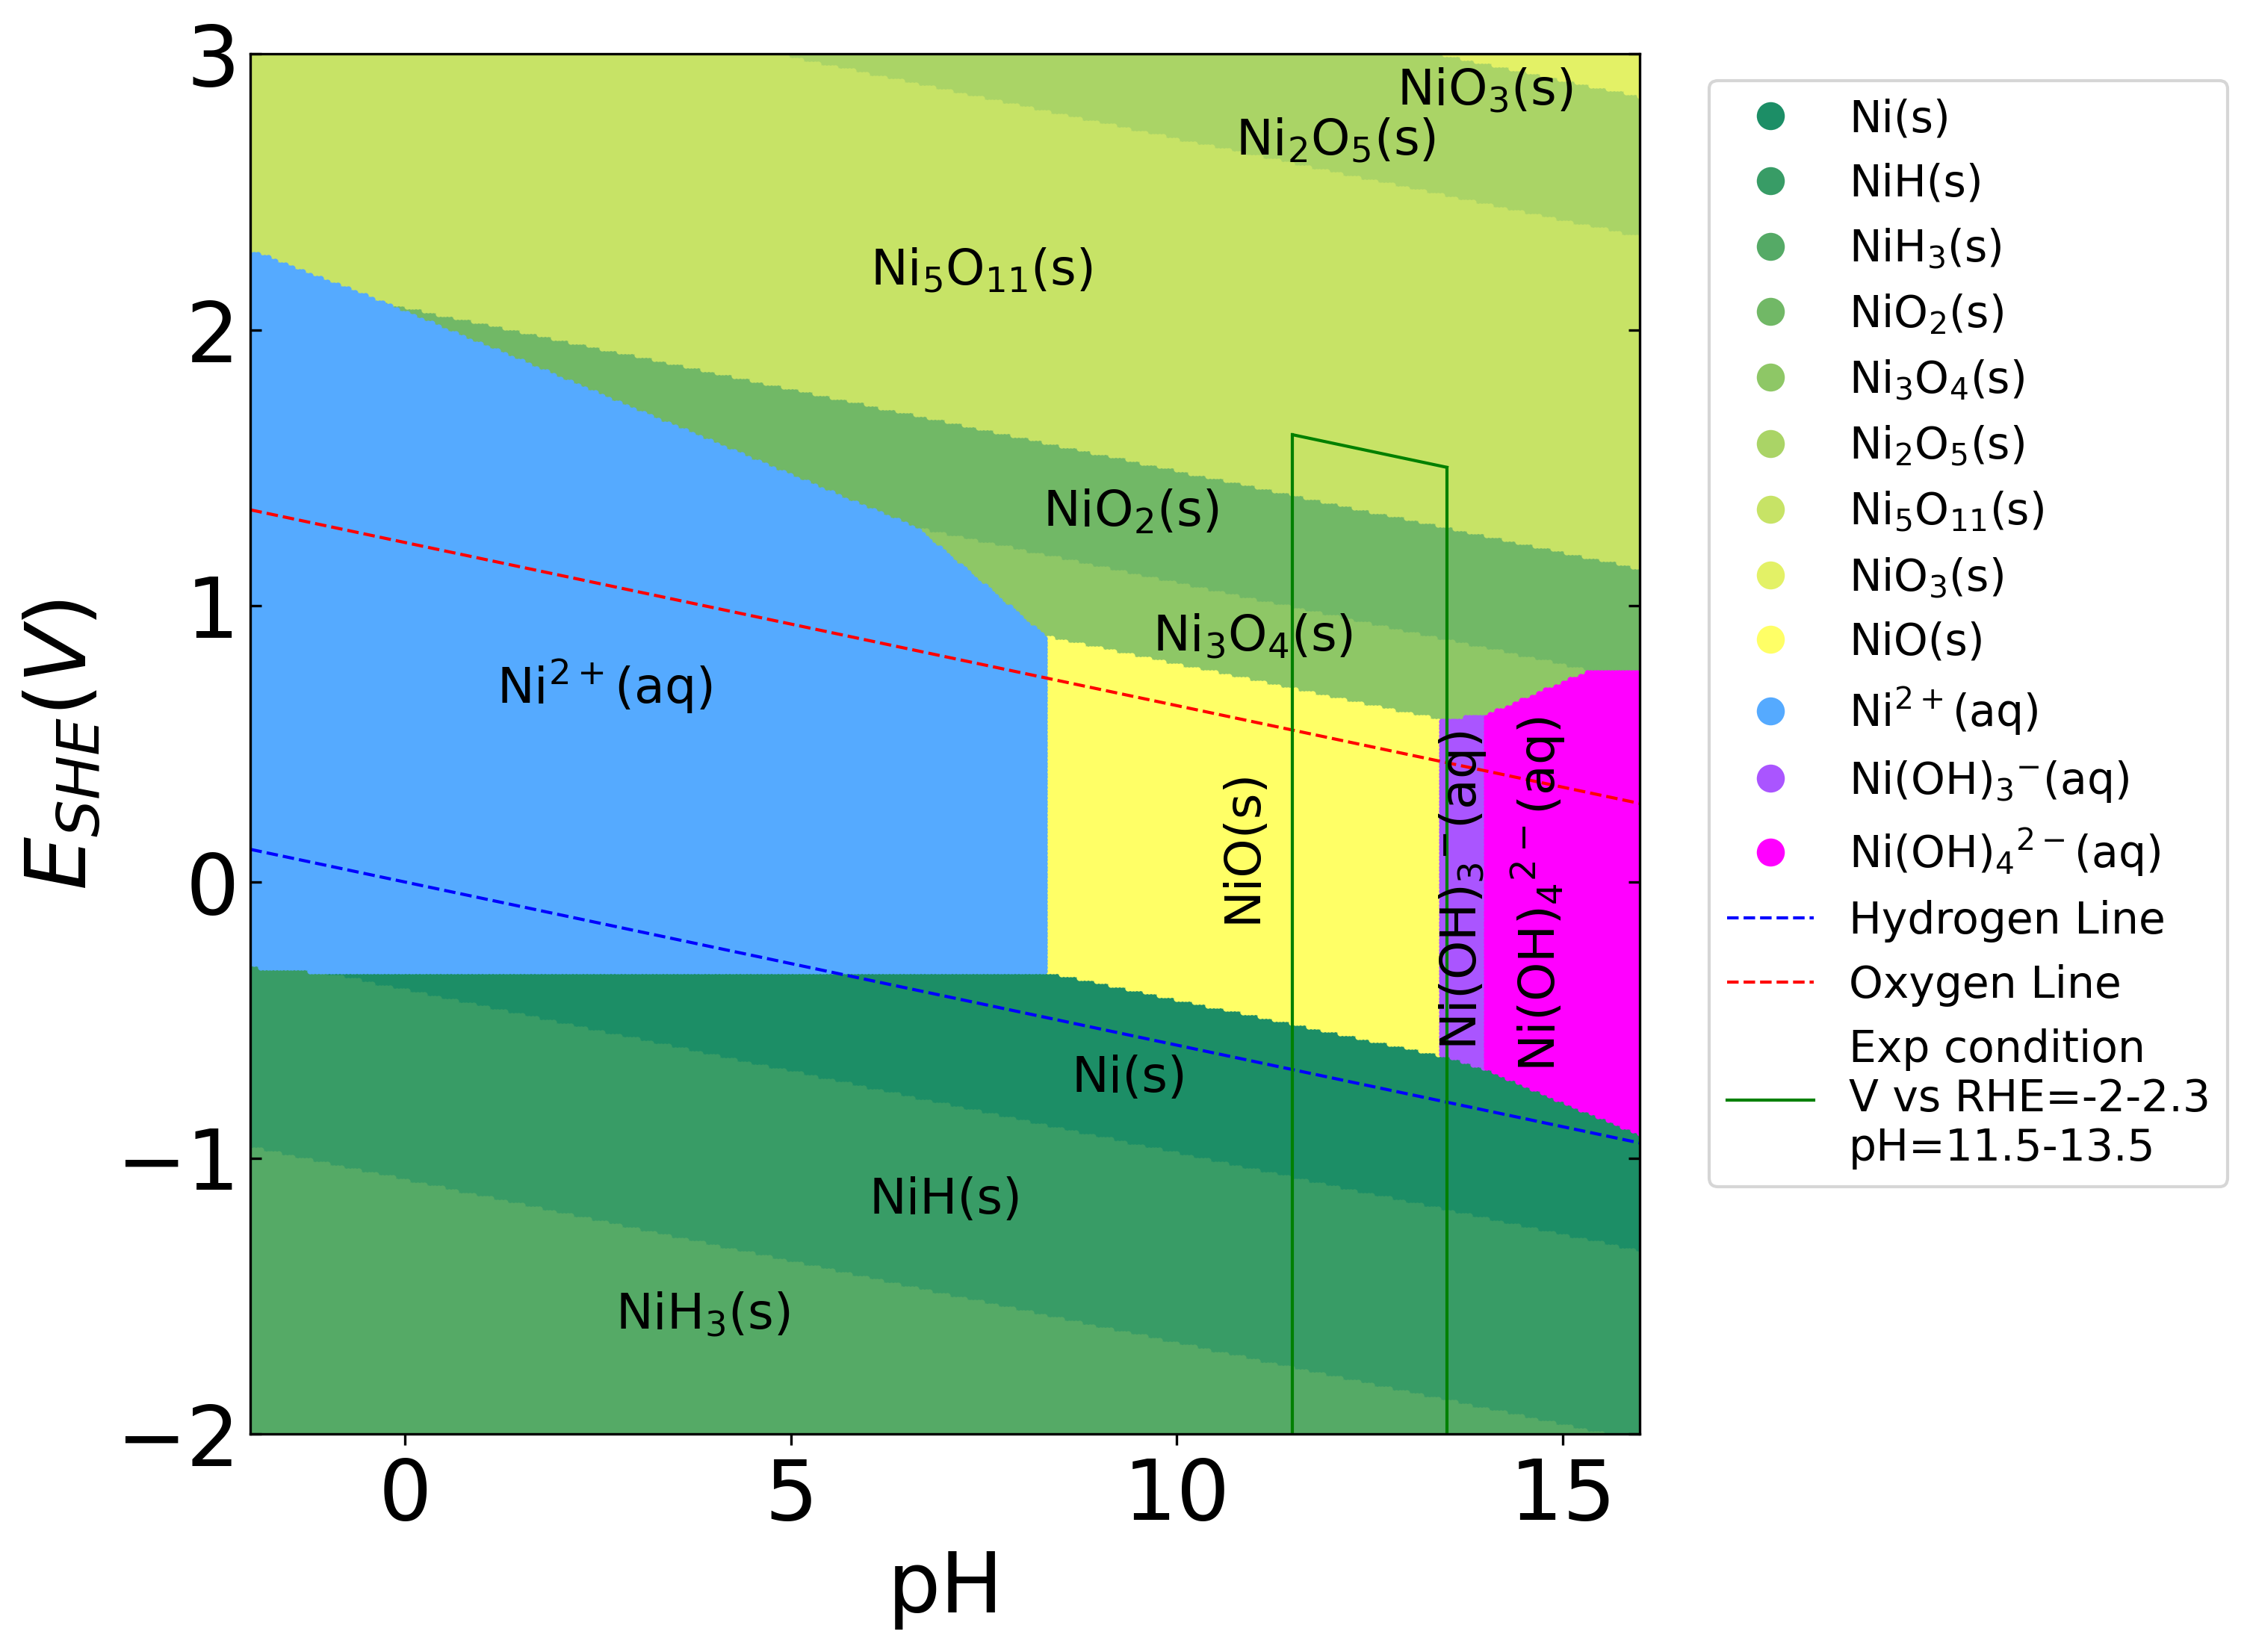
\includegraphics[width=0.7\textwidth]{Figures/pourbaix_diagrams/Ni-NH3-H2O_activity=1e-04_[NH3]=0M_[Gly]=0M_[CN]=0.png}
%     \caption{Pourbaix diagram for Ni at $[NH_3]_{initial}= 0.02M$, $[Gly]_{initial}=0.005M$. Green box indicates experimental condition at applied potential vs RHE = -2 to 2 V, pH = 11.5 to 13.5.}
%     \label{fig:Ni_Pourbaix_NH3_Gly_SI}
% \end{figure}
% \begin{figure}[htbp]
%     \centering
%     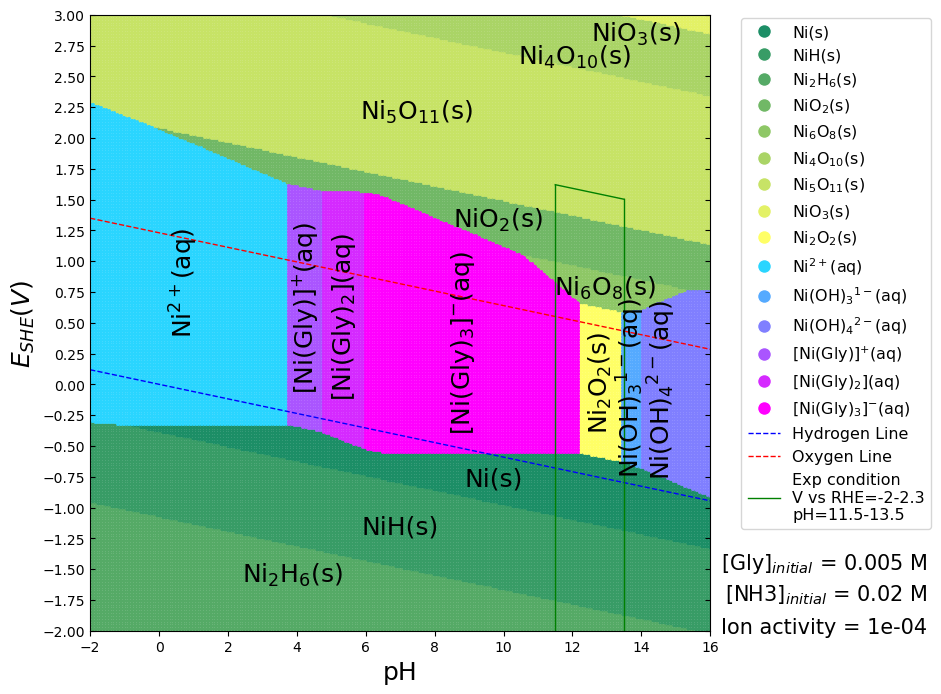
\includegraphics[width=0.7\textwidth]{Figures/pourbaix_diagrams/Ni-NH3-H2O_activity=1e-04_[NH3]=0.02M_[Gly]=0.005M_[CN]=0.png}
%     \caption{Pourbaix diagram for Ni at $[NH_3]_{initial}= 0.02M$, $[Gly]_{initial}=0.005M$. Green box indicates experimental condition at applied potential vs RHE = -2 to 2 V, pH = 11.5 to 13.5.}
%     \label{fig:Ni_Pourbaix_NH3_Gly_SI}
% \end{figure}
% \begin{figure}[htbp]
%     \centering
%     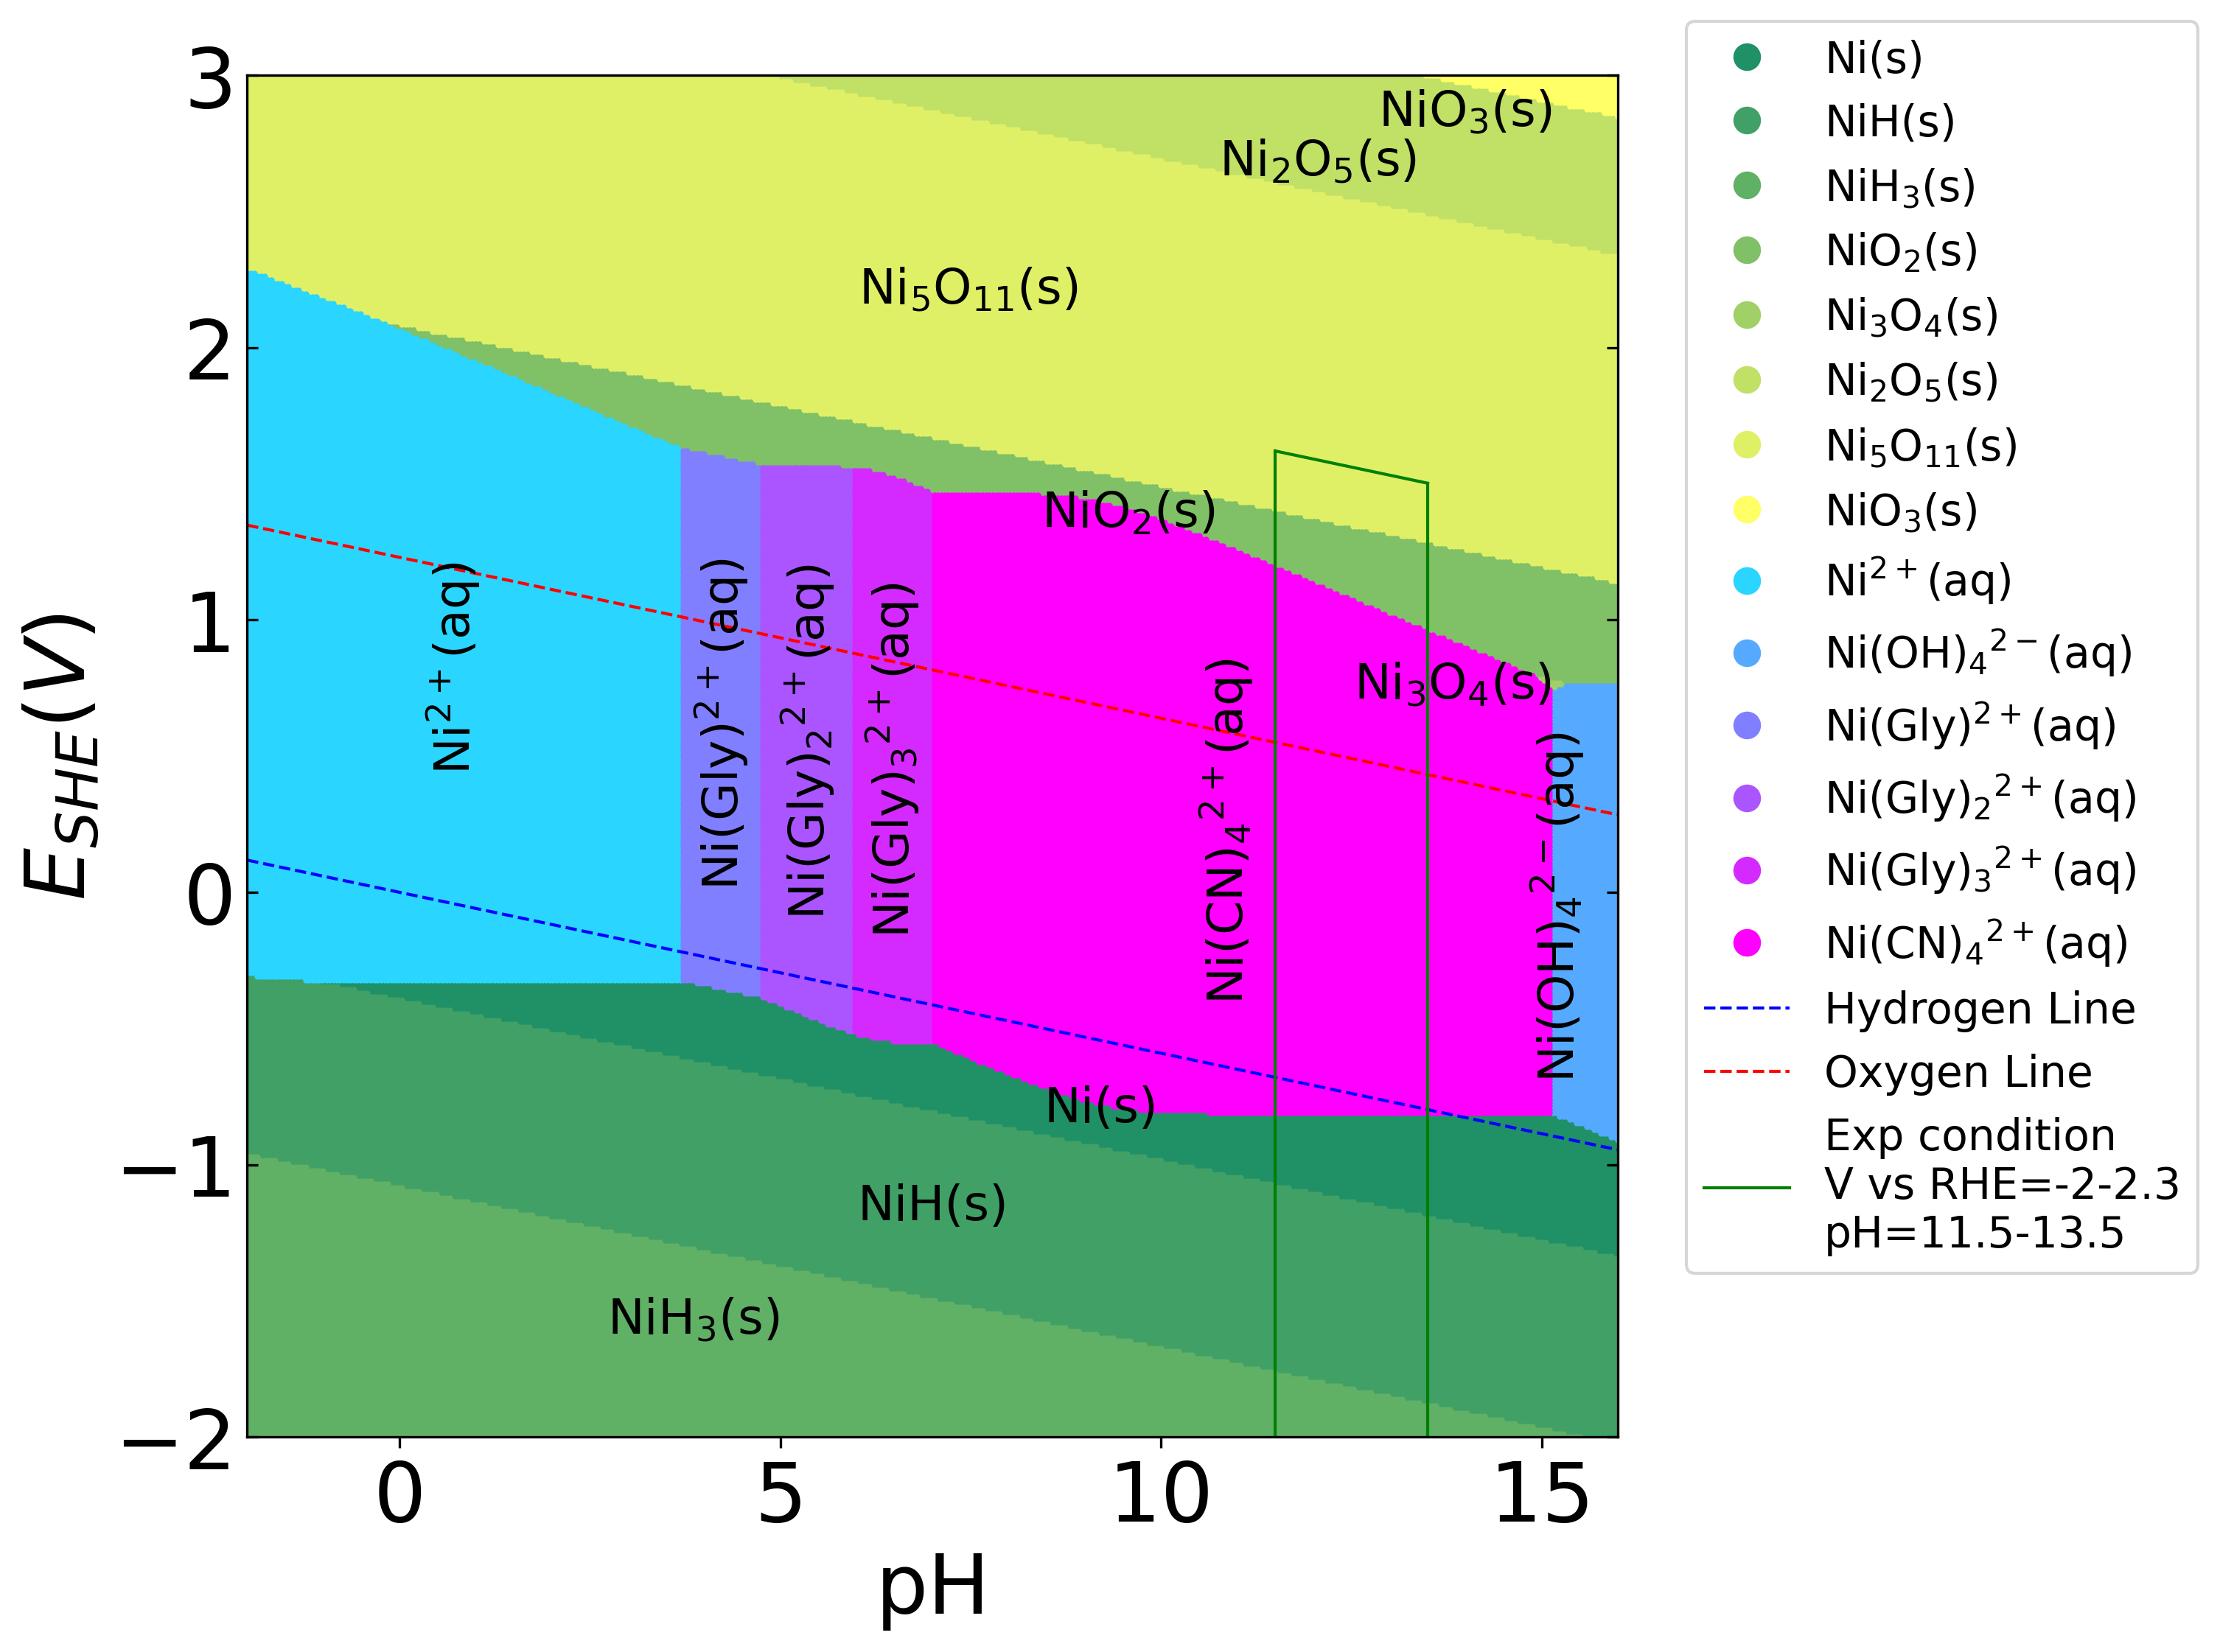
\includegraphics[width=0.7\textwidth]{Figures/pourbaix_diagrams/Ni-NH3-H2O_activity=1e-04_[NH3]=0.02M_[Gly]=0.005M_[CN]=0.0001.png}
%     \caption{Pourbaix diagram for Ni at $[NH_3]_{initial}= 0.02M$, $[Gly]_{initial}=0.005M$. Green box indicates experimental condition at applied potential vs RHE = -2 to 2 V, pH = 11.5 to 13.5.}
%     \label{fig:Ni_Pourbaix_NH3_Gly_SI}
% \end{figure}

%%%%%%%%%%%%%%%%%%%%%%%%%%%%%%%%% Cu %%%%%%%%%%%%%%%%%%%%%%%%%%%%%%%%%
% \begin{figure}[htbp]
%     \centering
%     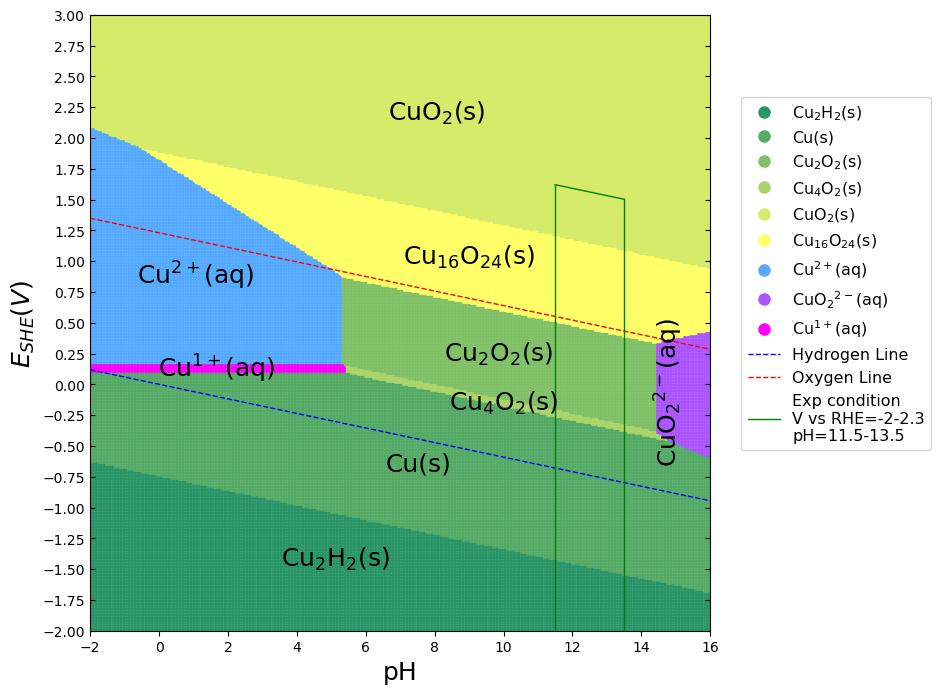
\includegraphics[width=0.7\textwidth]{Figures/pourbaix_diagrams/Cu-NH3-H2O_activity=1e-04_[NH3]=0M_[Gly]=0M_[CN]=0.png}
%     \caption{Pourbaix diagram for Cu at $[NH_3]_{initial}= 0.02M$, $[Gly]_{initial}=0.005M$. Green box indicates experimental condition at applied potential vs RHE = -2 to 2 V, pH = 11.5 to 13.5.}
%     \label{fig:Cu_Pourbaix_NH3_Gly_SI}
% \end{figure}
% \begin{figure}[htbp]
%     \centering
%     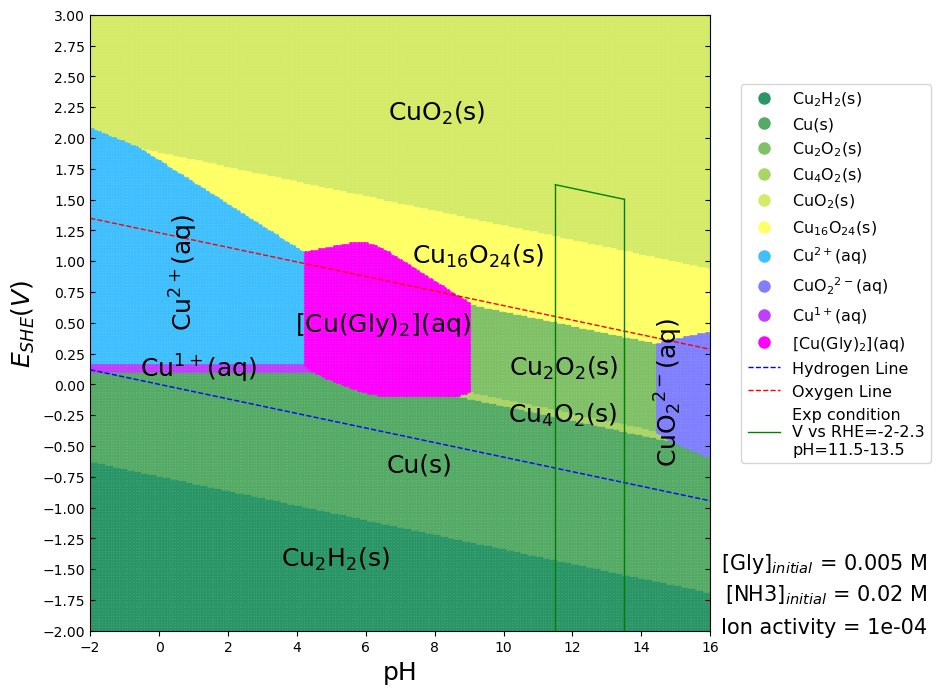
\includegraphics[width=0.7\textwidth]{Figures/pourbaix_diagrams/Cu-NH3-H2O_activity=1e-04_[NH3]=0.02M_[Gly]=0.005M_[CN]=0.png}
%     \caption{Pourbaix diagram for Cu at $[NH_3]_{initial}= 0.02M$, $[Gly]_{initial}=0.005M$. Green box indicates experimental condition at applied potential vs RHE = -2 to 2 V, pH = 11.5 to 13.5.}
%     \label{fig:Cu_Pourbaix_NH3_Gly_SI}
% \end{figure}
% \begin{figure}[htbp]
%     \centering
%     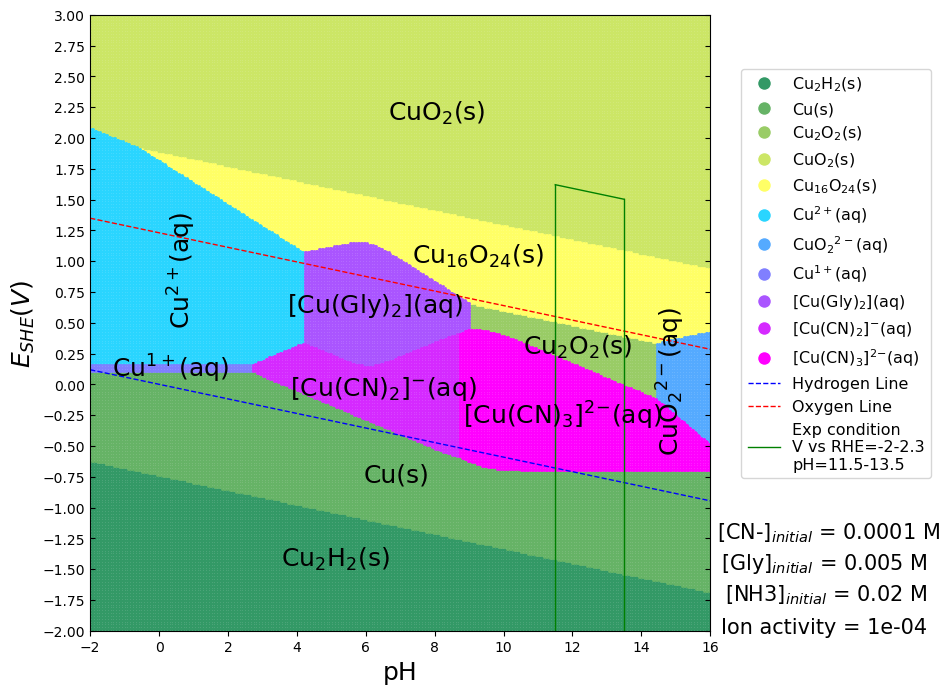
\includegraphics[width=0.7\textwidth]{Figures/pourbaix_diagrams/Cu-NH3-H2O_activity=1e-04_[NH3]=0.02M_[Gly]=0.005M_[CN]=0.0001.png}
%     \caption{Pourbaix diagram for Cu at $[NH_3]_{initial}= 0.02M$, $[Gly]_{initial}=0.005M$. Green box indicates experimental condition at applied potential vs RHE = -2 to 2 V, pH = 11.5 to 13.5.}
%     \label{fig:Cu_Pourbaix_NH3_Gly_SI}
% \end{figure}

%%%%%%%%%%%%%%%%%%%%%%%%%%%%%%%%% Pd %%%%%%%%%%%%%%%%%%%%%%%%%%%%%%%%%
% \begin{figure}[htbp]
%     \centering
%     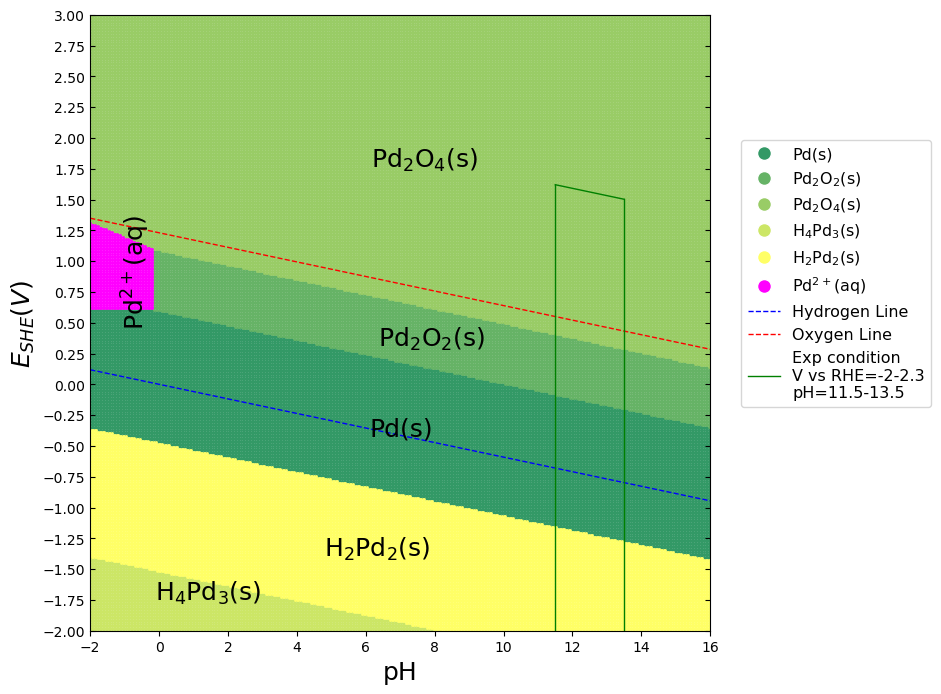
\includegraphics[width=0.7\textwidth]{Figures/pourbaix_diagrams/Pd-NH3-H2O_activity=1e-04_[NH3]=0M_[Gly]=0M_[CN]=0.png}
%     \caption{Pourbaix diagram for Pd at $[NH_3]_{initial}= 0.02M$, $[Gly]_{initial}=0.005M$. Green box indicates experimental condition at applied potential vs RHE = -2 to 2 V, pH = 11.5 to 13.5.}
%     \label{fig:Pd_Pourbaix_NH3_Gly_SI}
% \end{figure}
% \begin{figure}[htbp]
%     \centering
%     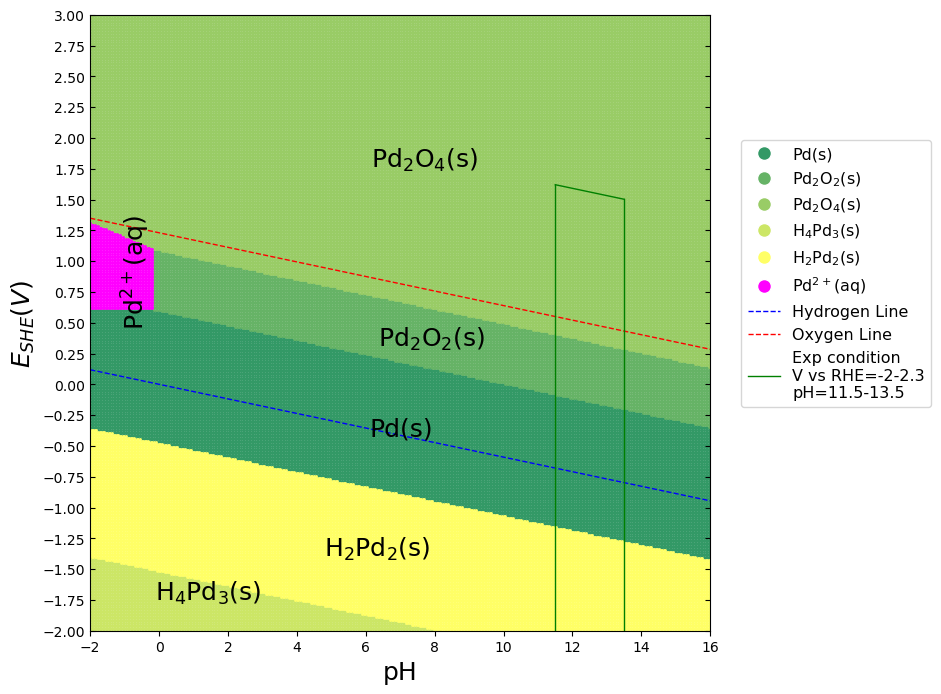
\includegraphics[width=0.7\textwidth]{Figures/pourbaix_diagrams/Pd-NH3-H2O_activity=1e-04_[NH3]=0.02M_[Gly]=0.005M_[CN]=0.png}
%     \caption{Pourbaix diagram for Pd at $[NH_3]_{initial}= 0.02M$, $[Gly]_{initial}=0.005M$. Green box indicates experimental condition at applied potential vs RHE = -2 to 2 V, pH = 11.5 to 13.5.}
%     \label{fig:Pd_Pourbaix_NH3_Gly_SI}
% \end{figure}
% \begin{figure}[htbp]
%     \centering
%     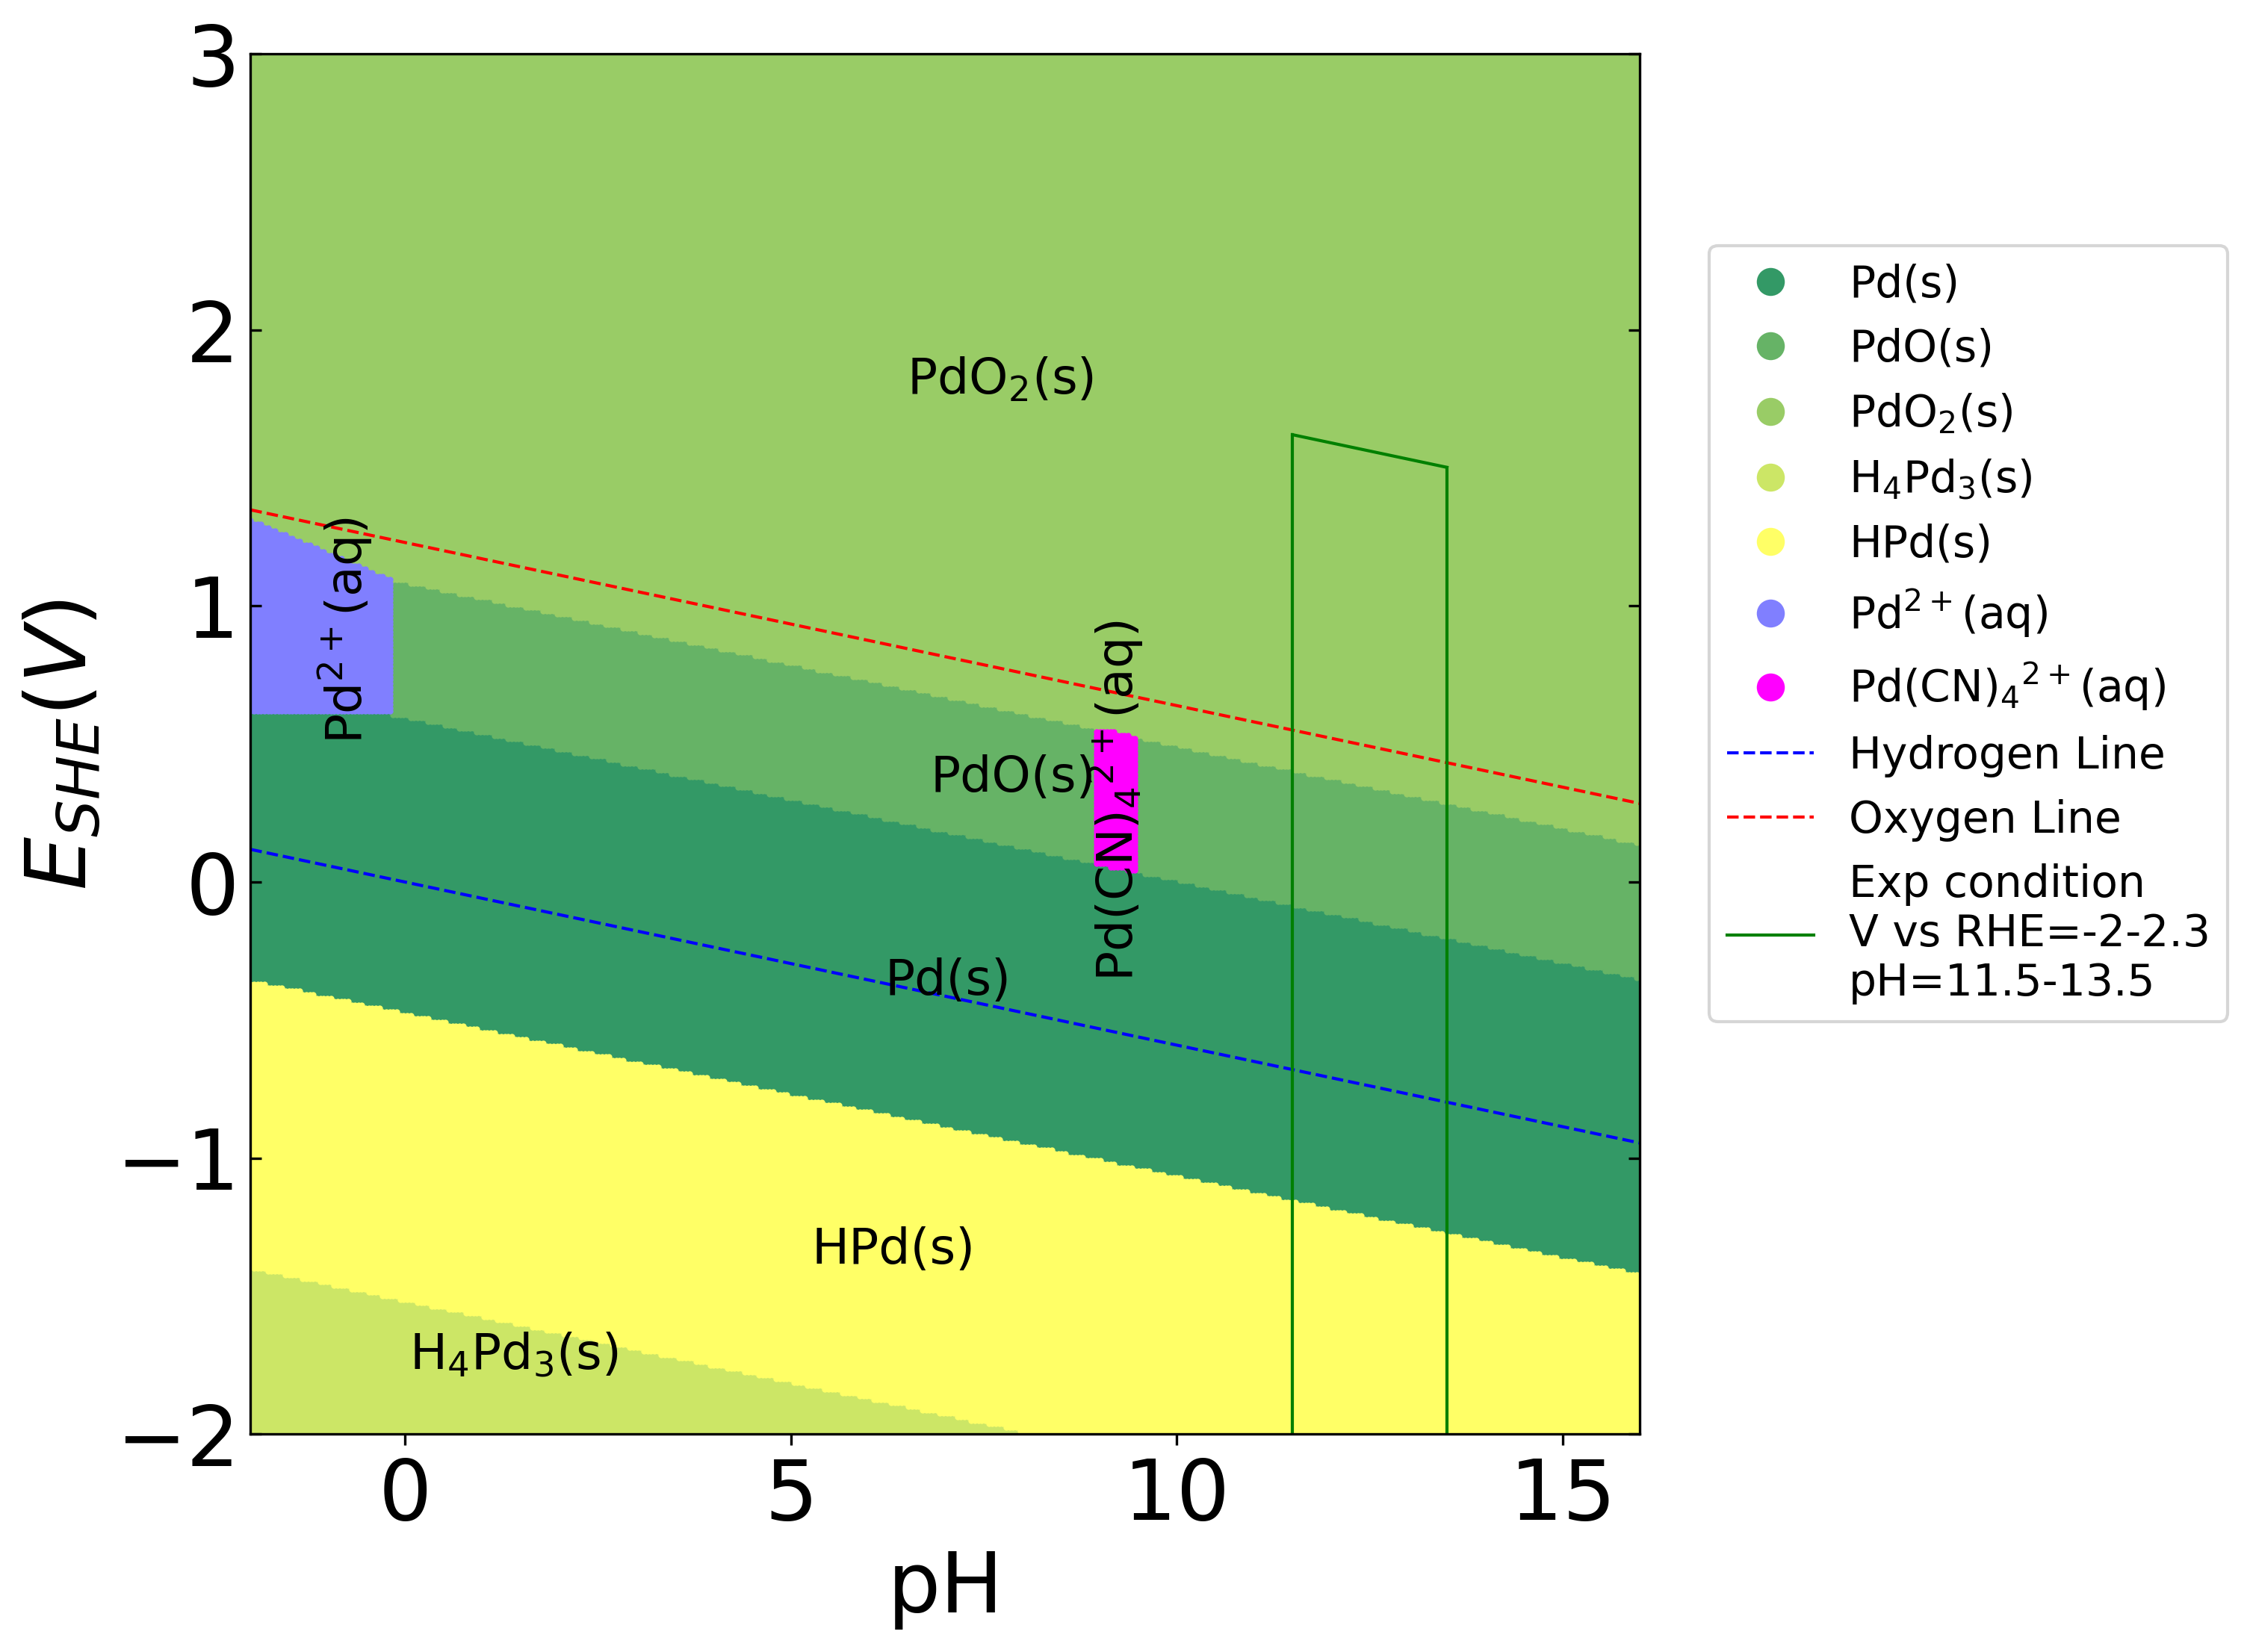
\includegraphics[width=0.7\textwidth]{Figures/pourbaix_diagrams/Pd-NH3-H2O_activity=1e-04_[NH3]=0.02M_[Gly]=0.005M_[CN]=0.0001.png}
%     \caption{Pourbaix diagram for Pd at $[NH_3]_{initial}= 0.02M$, $[Gly]_{initial}=0.005M$. Green box indicates experimental condition at applied potential vs RHE = -2 to 2 V, pH = 11.5 to 13.5.}
%     \label{fig:Pd_Pourbaix_NH3_Gly_SI}
% \end{figure}

\begin{figure}[htbp]
    \centering
    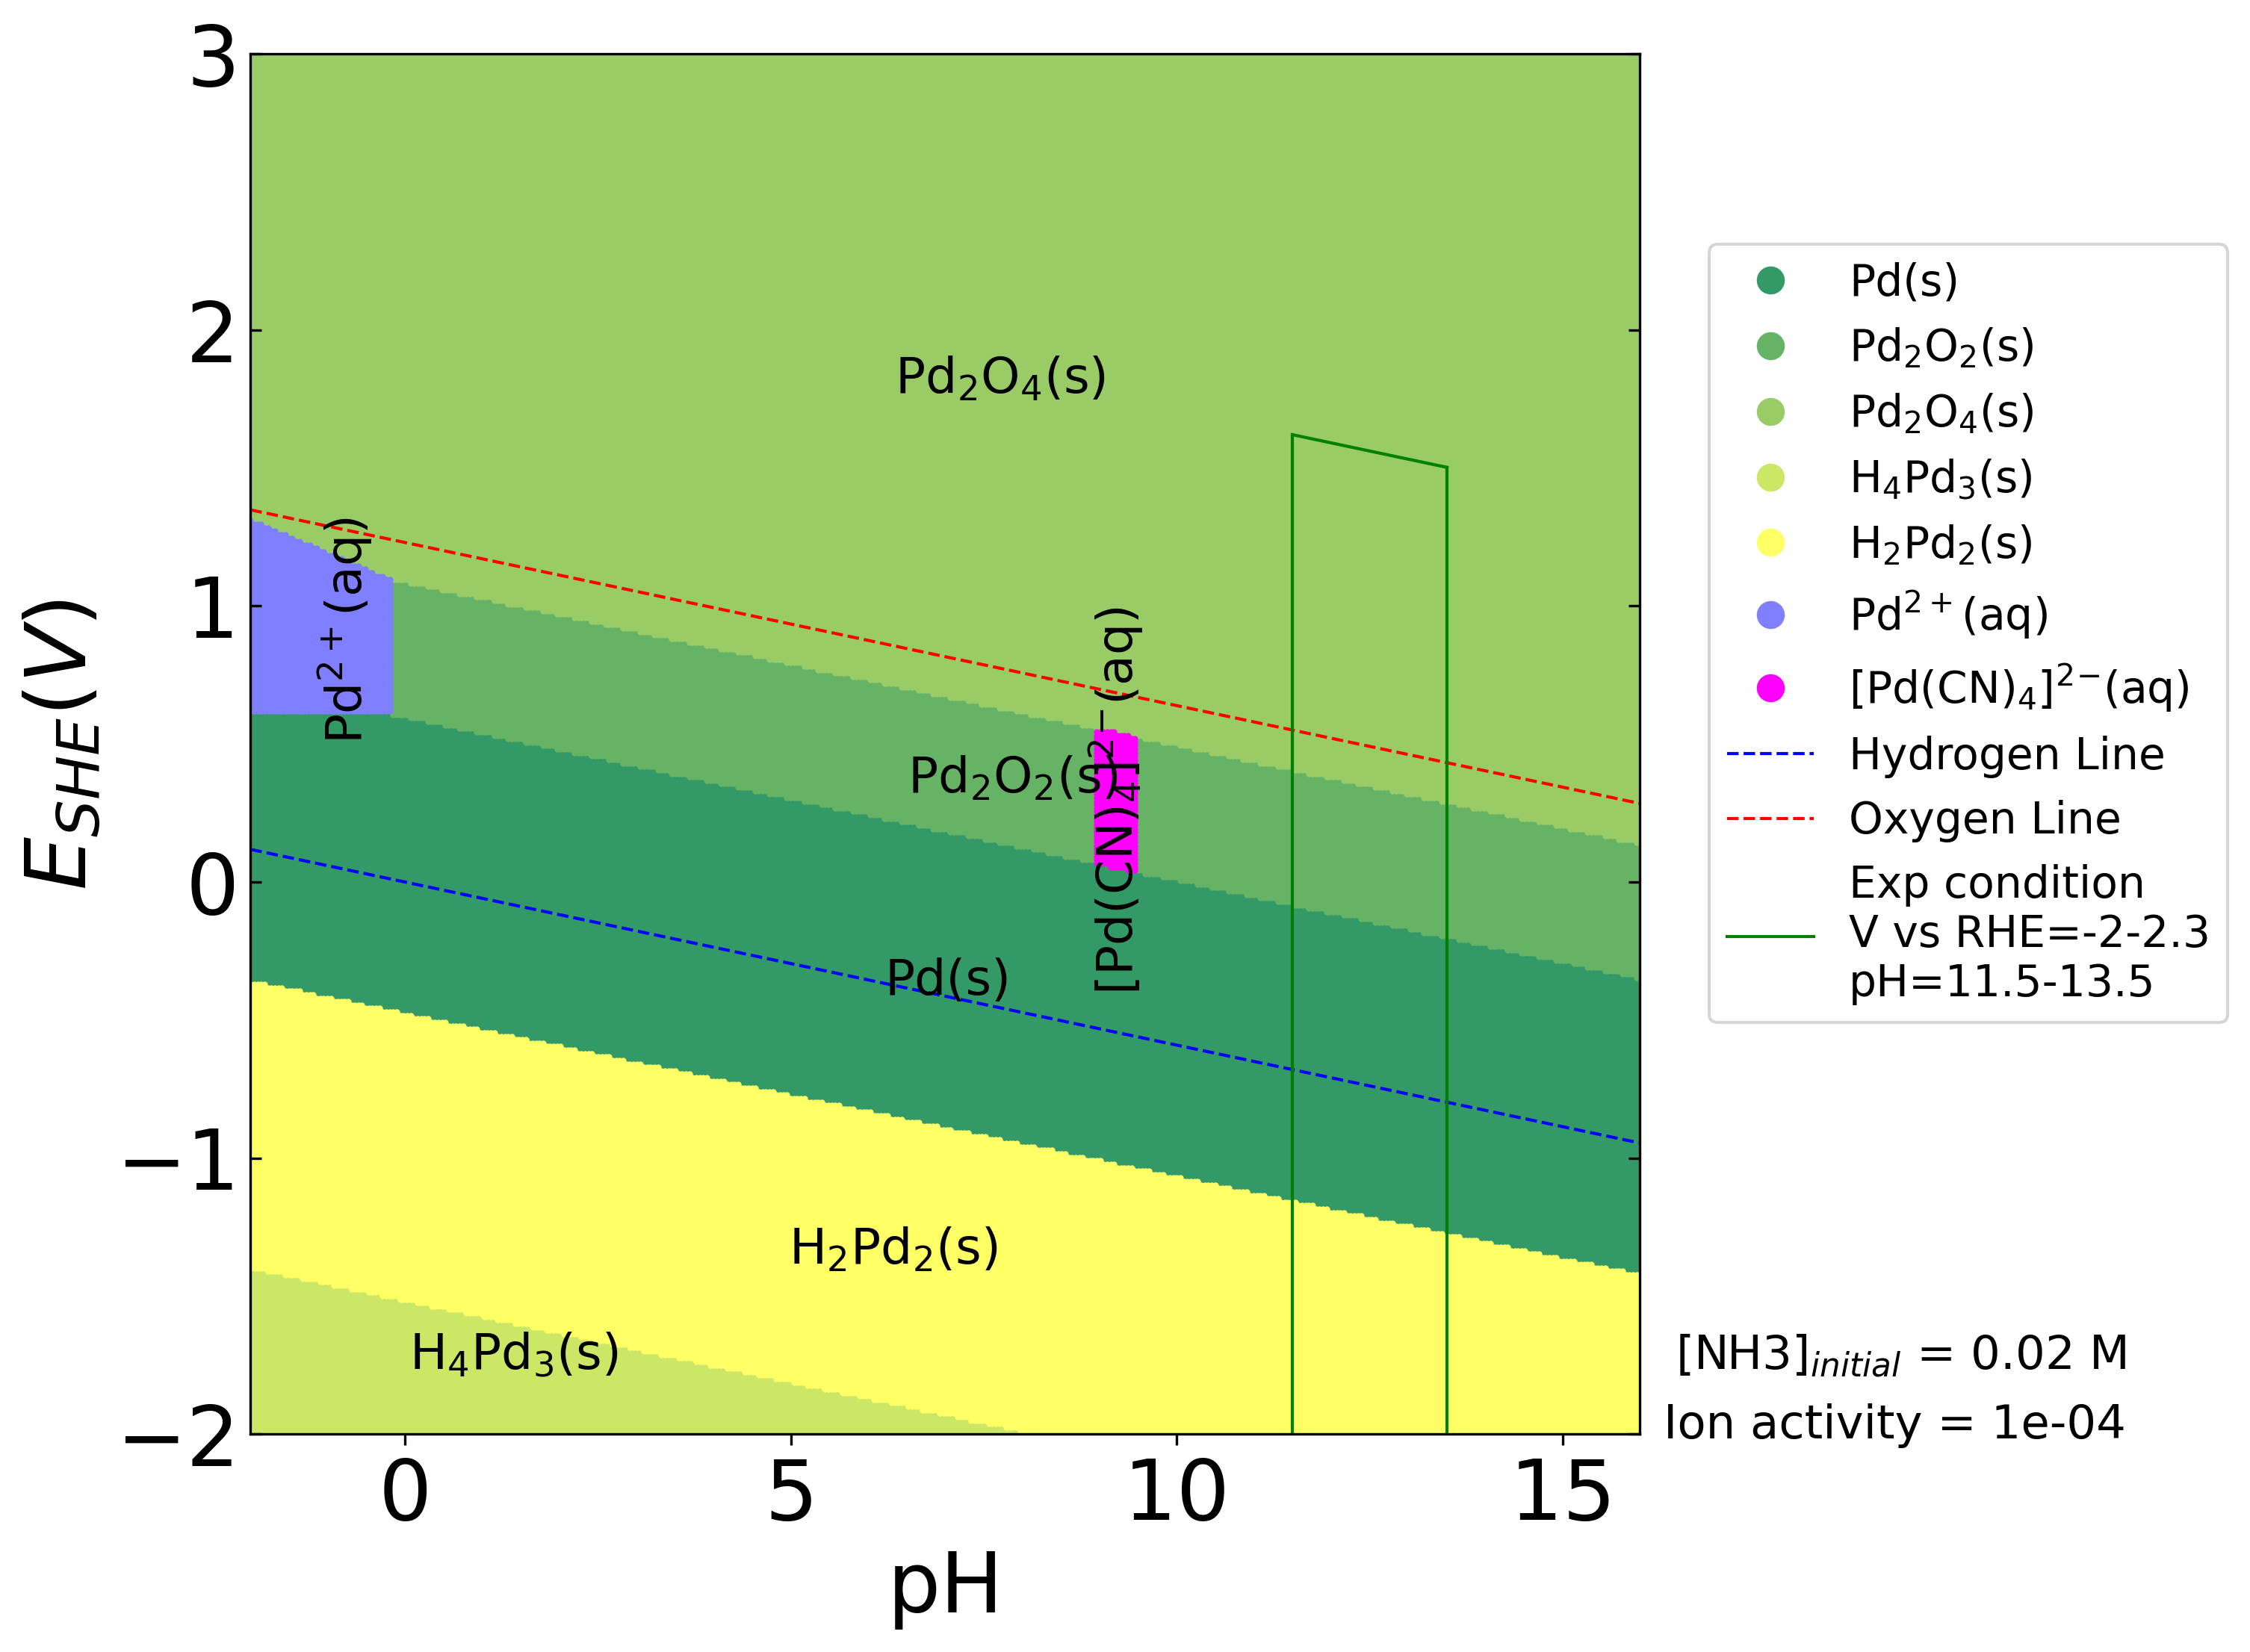
\includegraphics[width=0.7\textwidth]{Figures/pourbaix_diagrams/Pd-NH3-H2O_activity_Smith1989CriticalConstants_Pd_42.4=1e-04_[NH3]=0.02M_[Gly]=0.005M_[CN]=0.0001.png}
    \caption{Pourbaix diagram for Pd at $[NH_3]_{initial}= 0.02M$, $[Gly]_{initial}=0.005M$, and $[\ce{CN-}]_{initial}=1e^{-4}$M. \ce{[Pd(CN)4]^2-} formation energy calculated using stability constant $log\beta_4=42.4$ from Smith et al.\cite{Smith1989CriticalConstants} Green box indicates experimental condition at applied potential vs RHE = -2 to 2 V, pH = 11.5 to 13.5.}
    \label{fig:Pd_Pourbaix_Smith1989CriticalConstants_SI}
\end{figure}

%%%%%%%%%%%%%%%%%%%%%%%%%%%%%%%%% Pt %%%%%%%%%%%%%%%%%%%%%%%%%%%%%%%%%
% \begin{figure}[htbp]
%     \centering
%     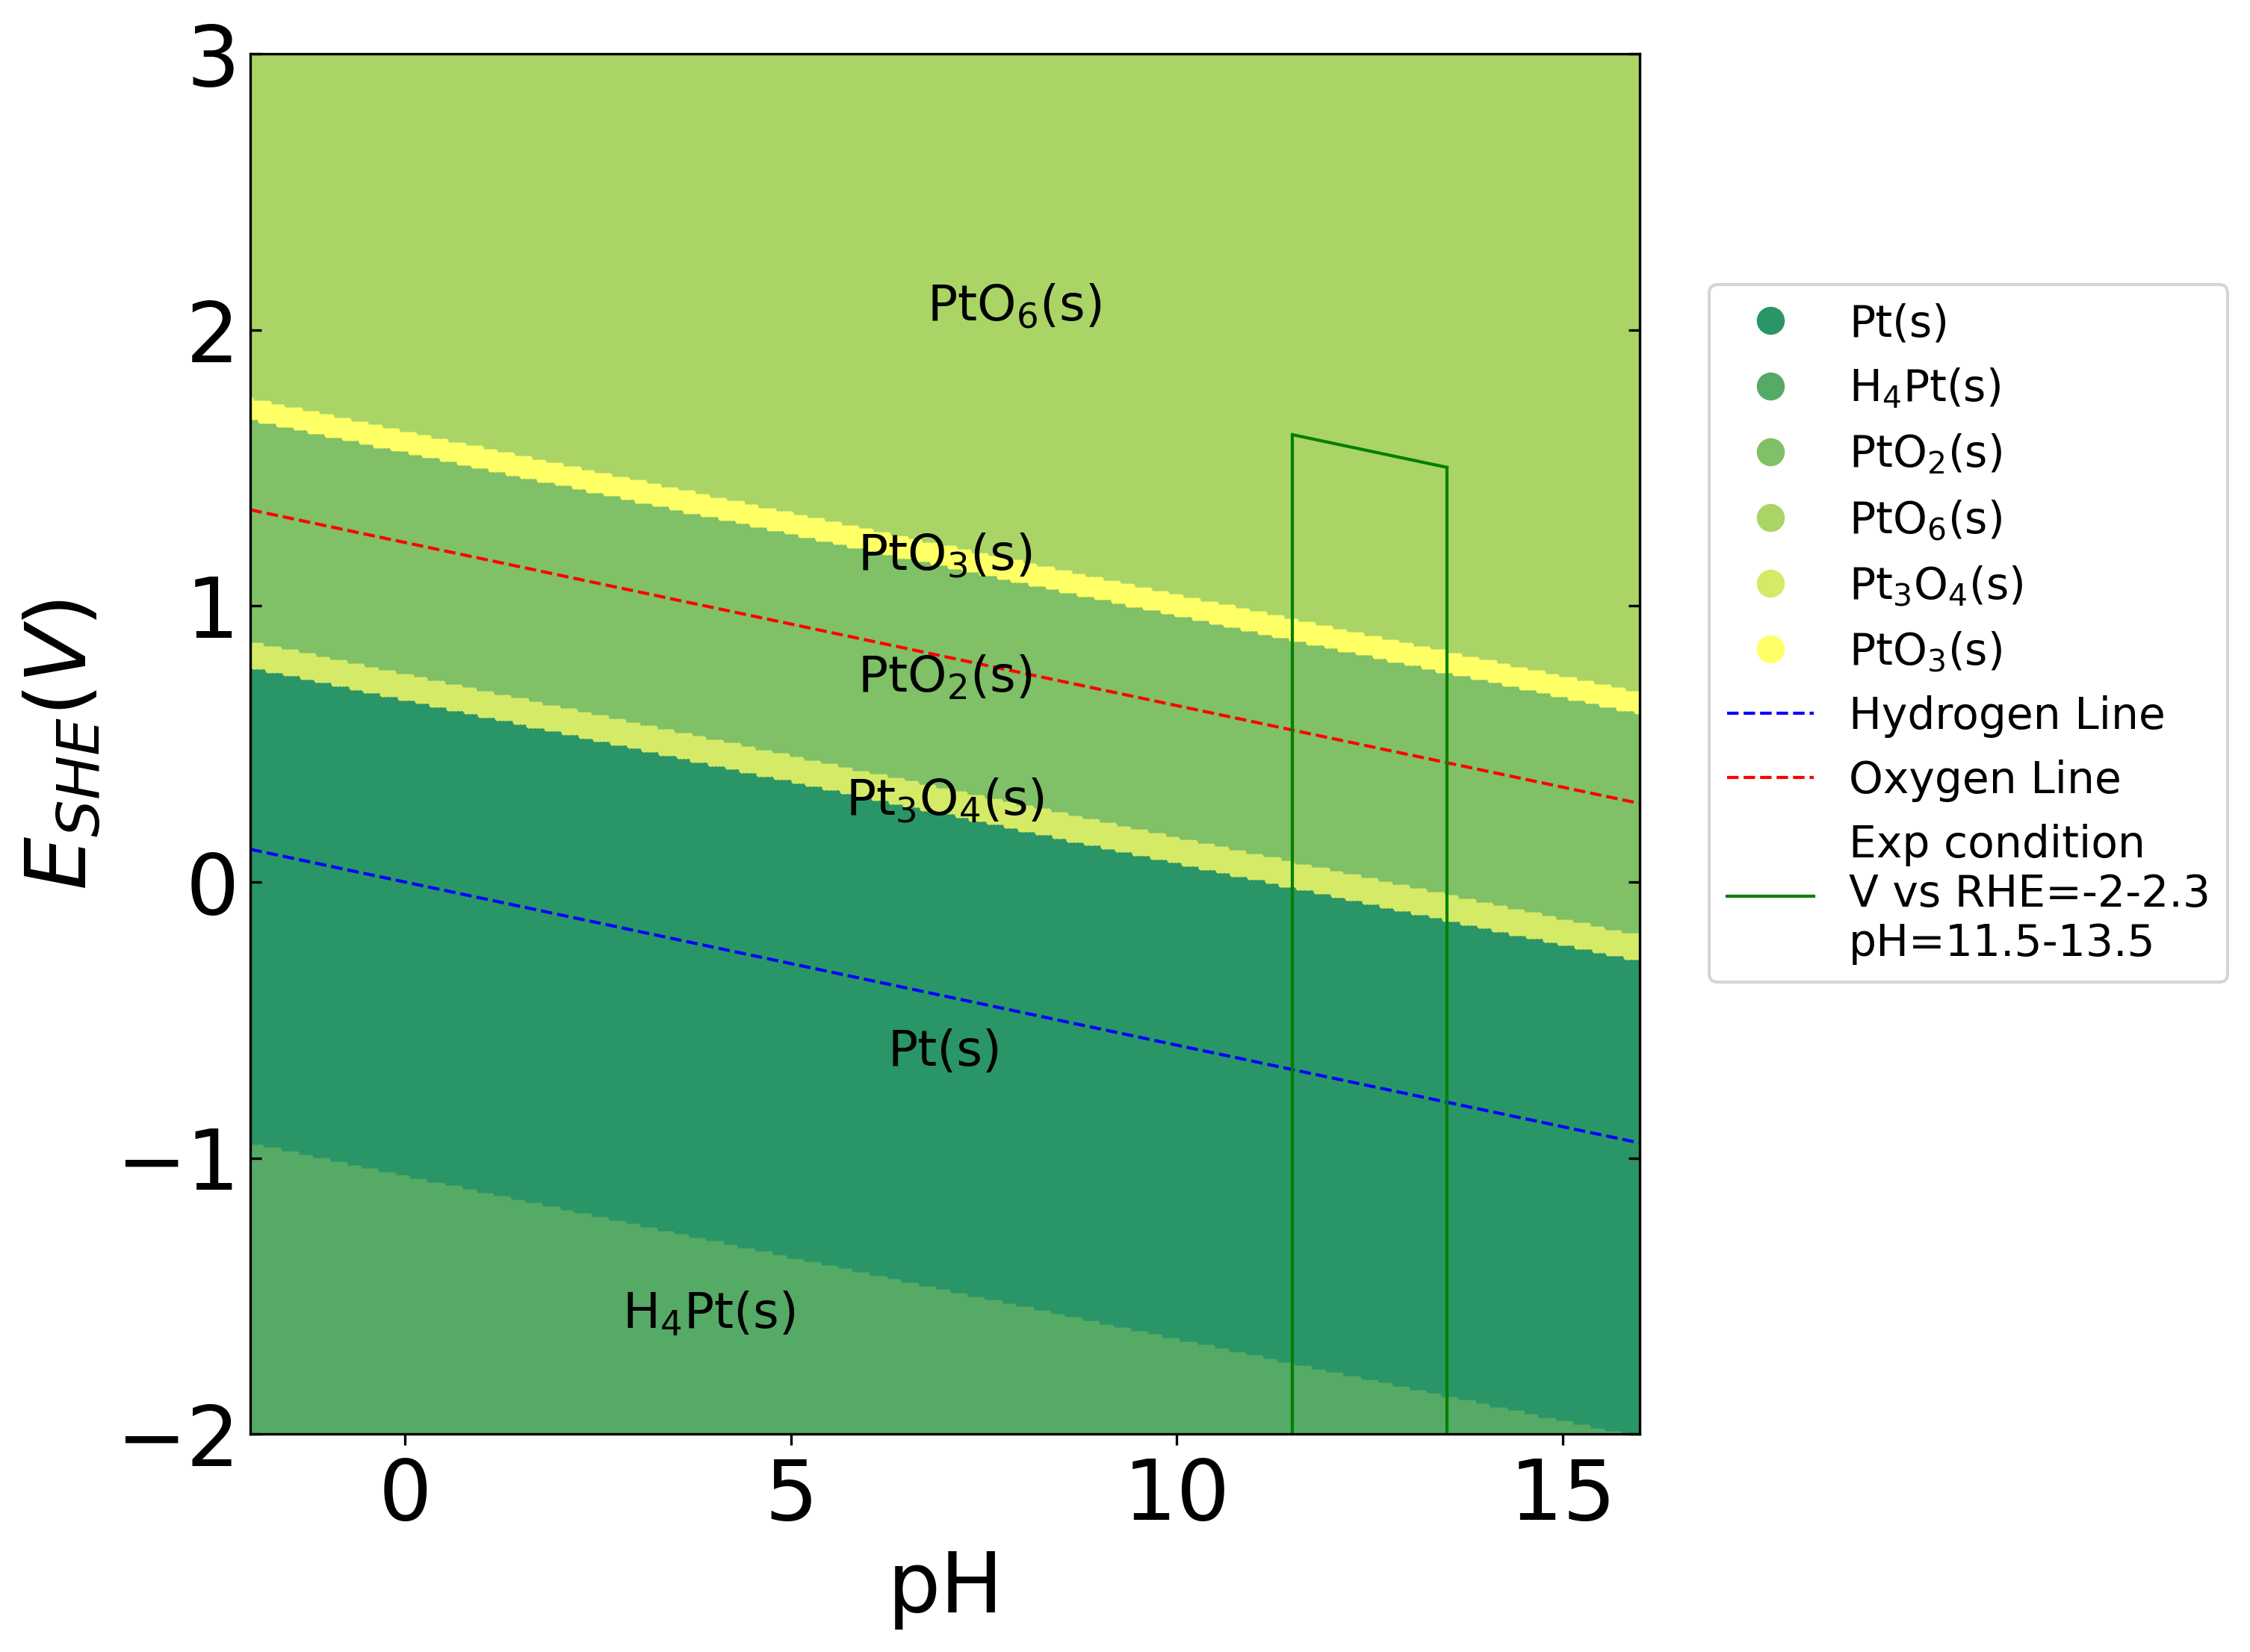
\includegraphics[width=0.7\textwidth]{Figures/pourbaix_diagrams/Pt-NH3-H2O_activity=1e-04_[NH3]=0M_[Gly]=0M_[CN]=0.png}
%     \caption{Pourbaix diagram for Pt at $[NH_3]_{initial}= 0.02M$, $[Gly]_{initial}=0.005M$. Green box indicates experimental condition at applied potential vs RHE = -2 to 2 V, pH = 11.5 to 13.5.}
%     \label{fig:Pt_Pourbaix_NH3_Gly_SI}
% \end{figure}
% \begin{figure}[htbp]
%     \centering
%     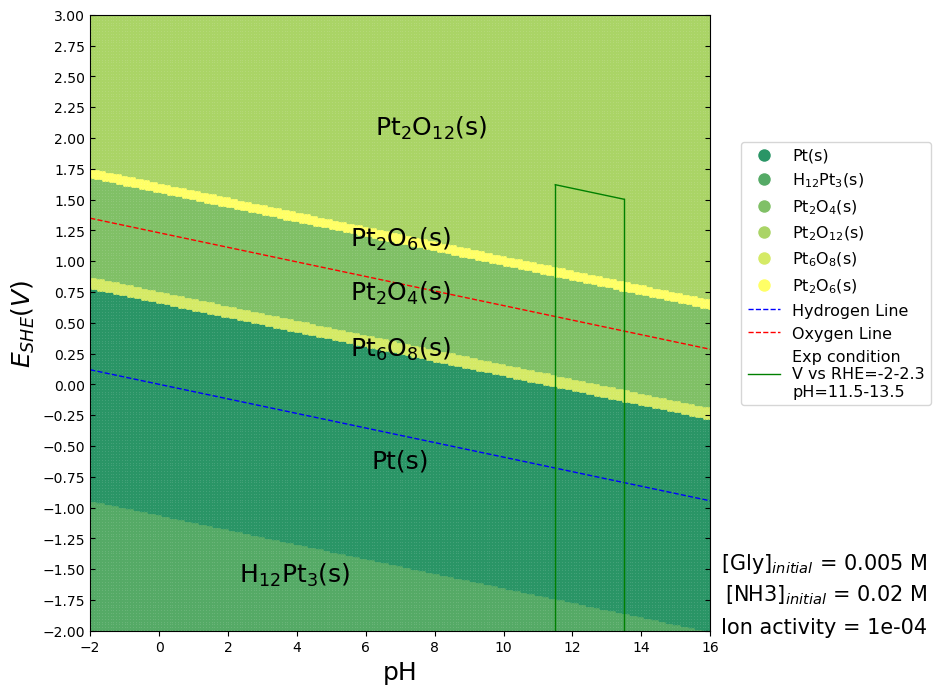
\includegraphics[width=0.7\textwidth]{Figures/pourbaix_diagrams/Pt-NH3-H2O_activity=1e-04_[NH3]=0.02M_[Gly]=0.005M_[CN]=0.png}
%     \caption{Pourbaix diagram for Pt at $[NH_3]_{initial}= 0.02M$, $[Gly]_{initial}=0.005M$. Green box indicates experimental condition at applied potential vs RHE = -2 to 2 V, pH = 11.5 to 13.5.}
%     \label{fig:Pt_Pourbaix_NH3_Gly_SI}
% \end{figure}
% \begin{figure}[htbp]
%     \centering
%     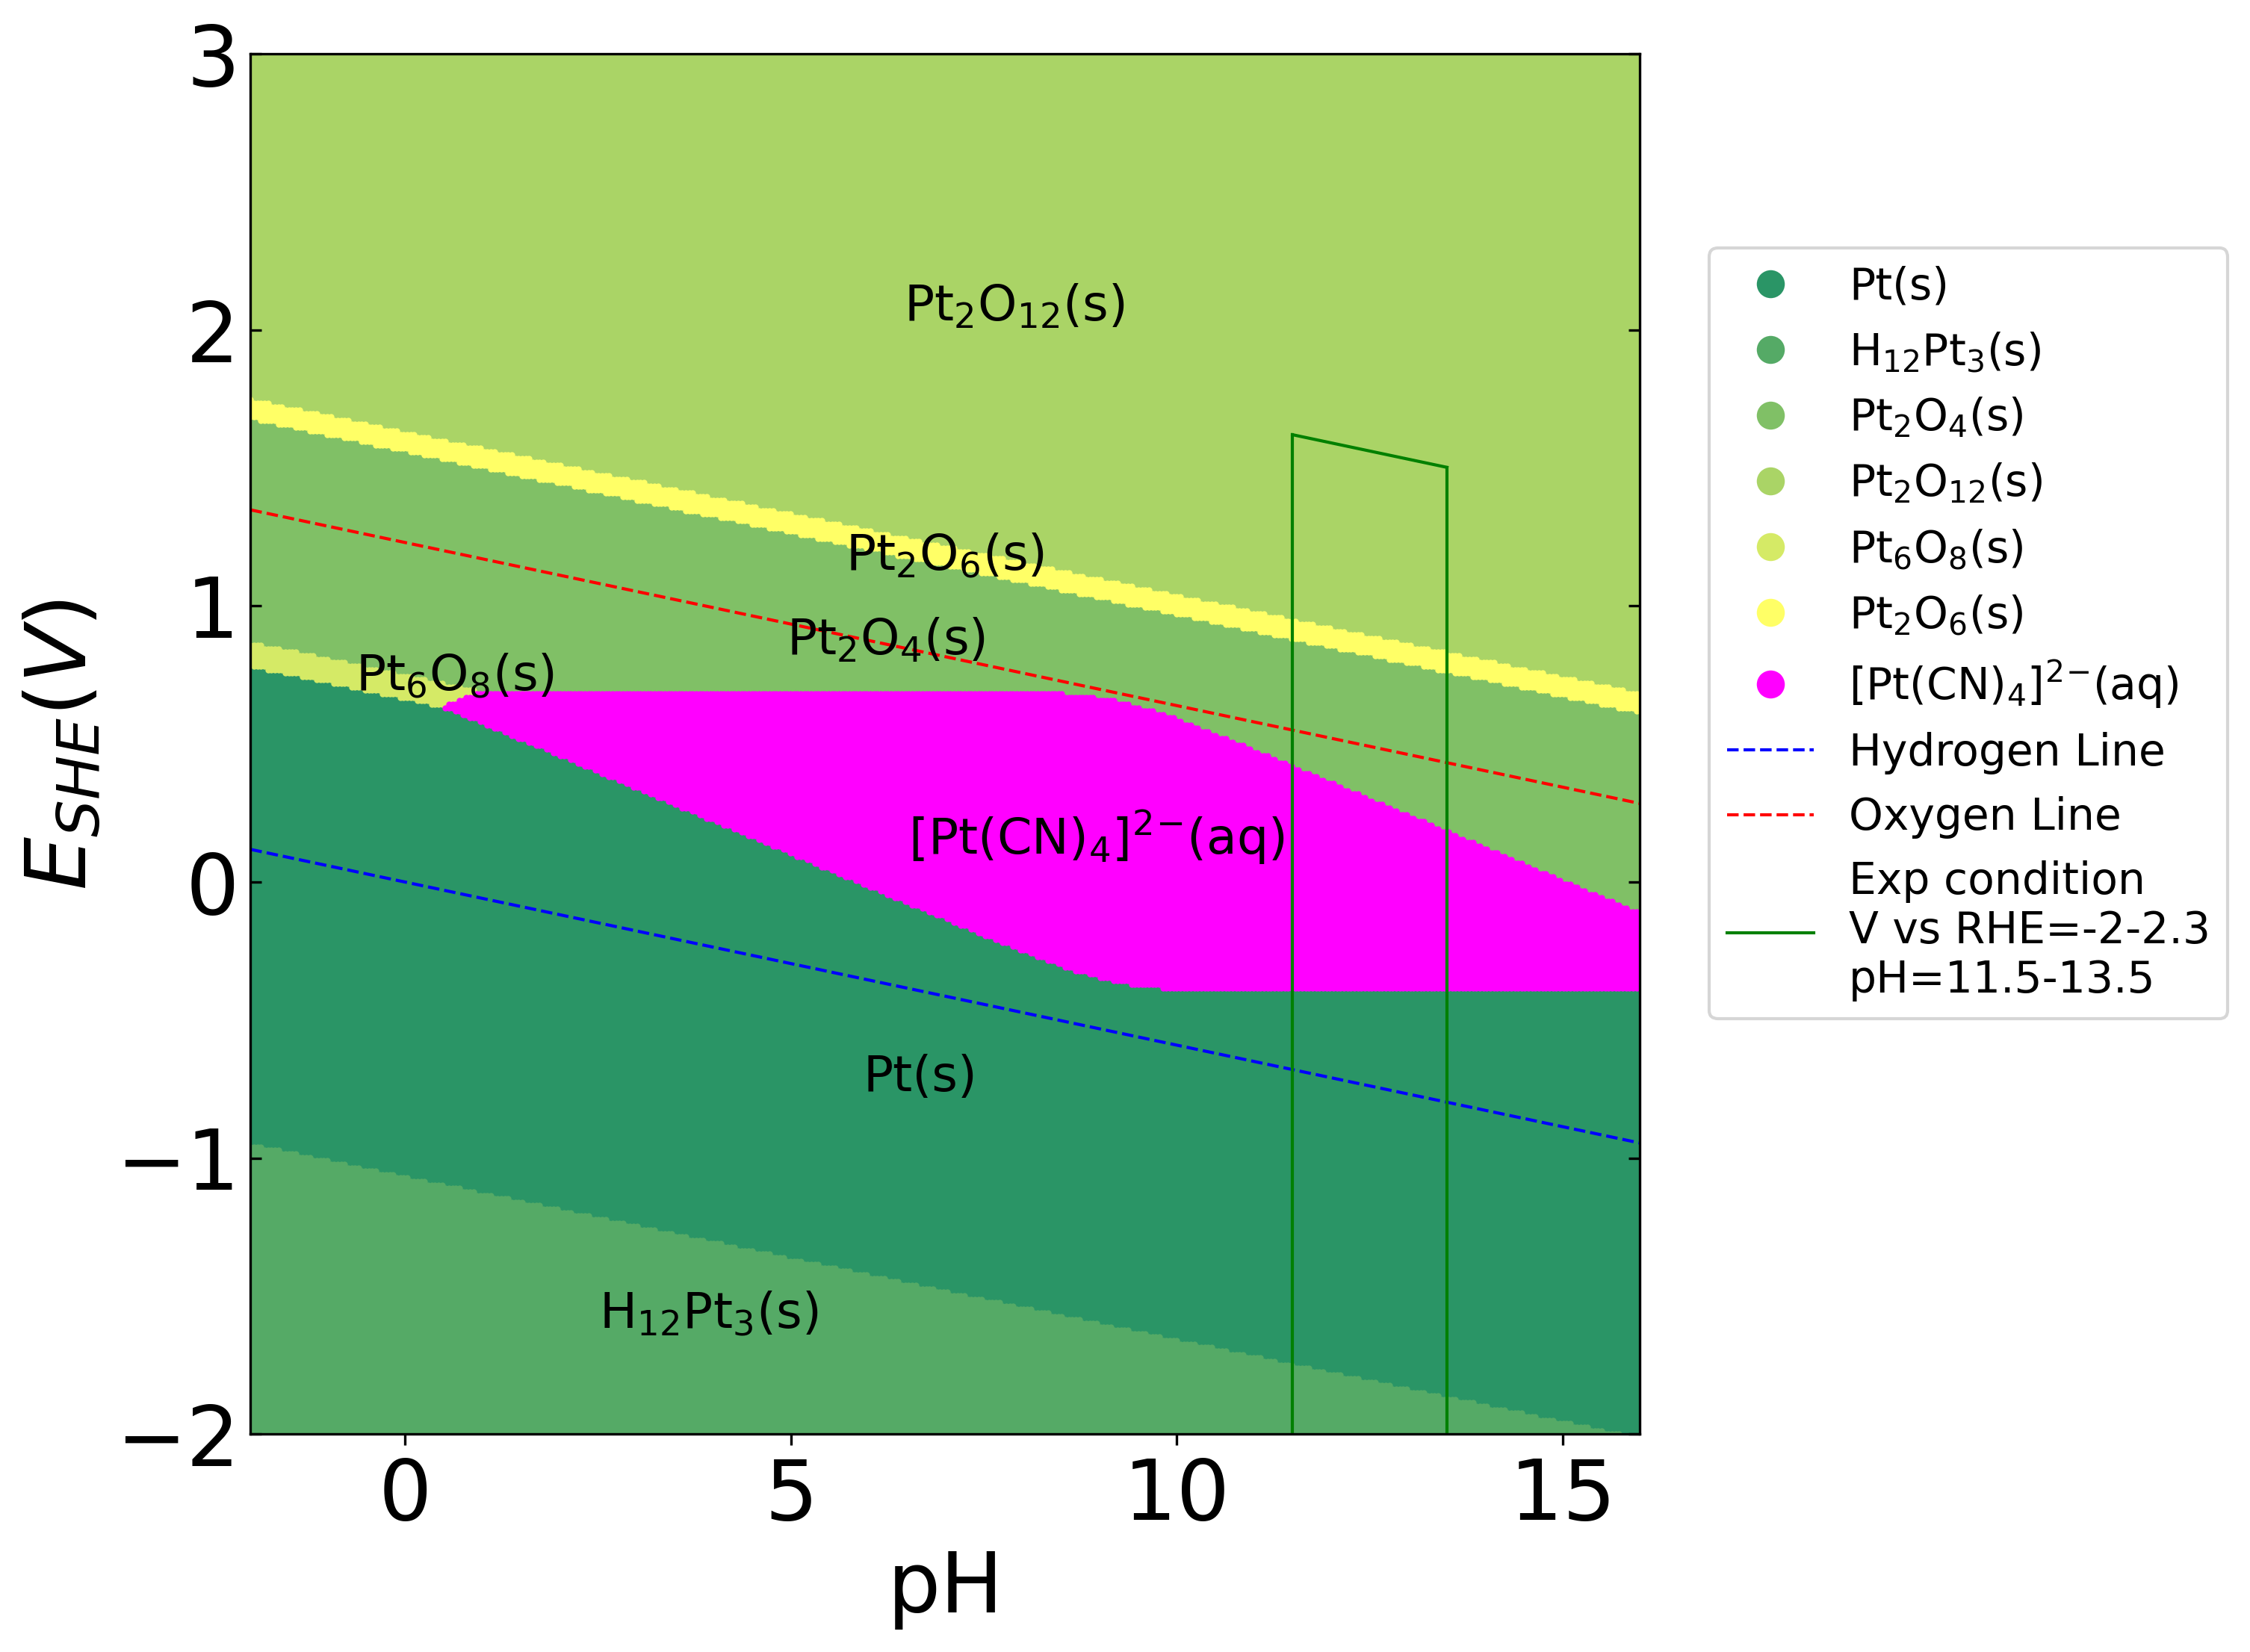
\includegraphics[width=0.7\textwidth]{Figures/pourbaix_diagrams/Pt-NH3-H2O_activity=1e-04_[NH3]=0.02M_[Gly]=0.005M_[CN]=0.0001.png}
%     \caption{Pourbaix diagram for Pt at $[NH_3]_{initial}= 0.02M$, $[Gly]_{initial}=0.005M$. Green box indicates experimental condition at applied potential vs RHE = -2 to 2 V, pH = 11.5 to 13.5.}
%     \label{fig:Pt_Pourbaix_NH3_Gly_SI}
% \end{figure}
\begin{figure}[htbp]
    \centering
    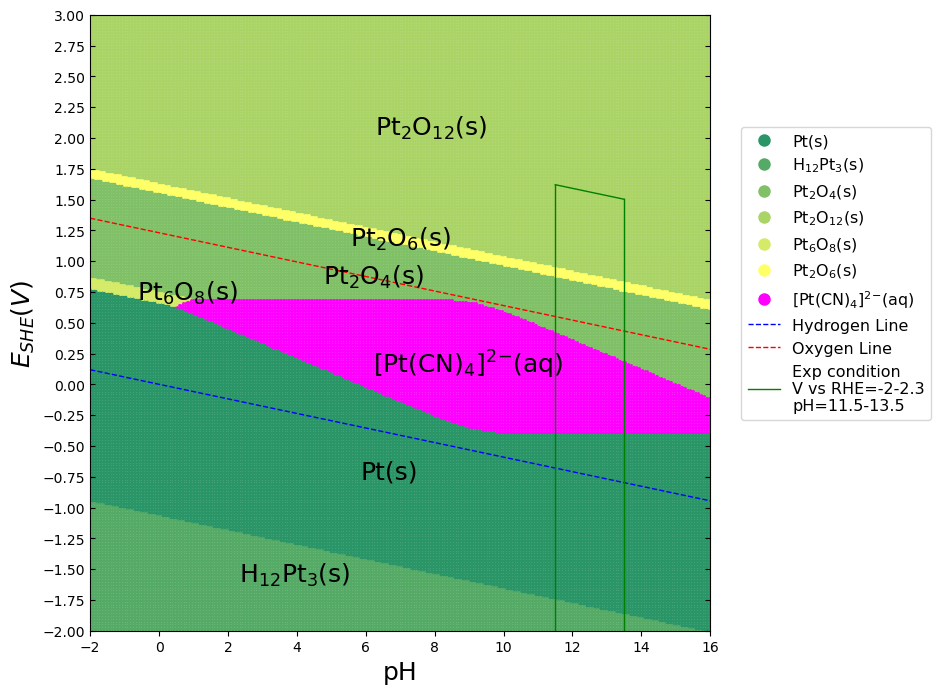
\includegraphics[width=0.7\textwidth]{Figures/pourbaix_diagrams/Pt-NH3-H2O_activity_Harrington_Pt_70=1e-04_[NH3]=0.02M_[Gly]=0.005M_[CN]=0.0001.png}
    \caption{Pourbaix diagram for Pt at $[NH_3]_{initial}= 0.02M$, $[Gly]_{initial}=0.005M$ and $[\ce{CN-}]_{initial}=1e^{-4}$M. \ce{[Pt(CN)4]^2-} formation energy calculated using estimated stability constant $log\beta_4=70$ by Harring et al.\cite{Harrington2005DeterminationIon} Green box indicates experimental condition at applied potential vs RHE = -2 to 2 V, pH = 11.5 to 13.5.}
    \label{fig:Pt_Pourbaix_Harrington_SI}
\end{figure}

\newpage
\clearpage
\begin{longtable}{|p{4cm}|p{4cm}|p{3cm}|p{3cm}|}
\caption{Formation energies of species for \ce{NH3} complexes.} 
\label{tab:NH3_complex_energies}
\\
\hline
\textbf{Species} & \textbf{Metal ion} & \textbf{\( \Delta G^\circ_{298} \) (eV)} & \textbf{Reference} \\ \hline
\endfirsthead
\caption*{Table \thetable\ continued from previous pages.} \\
\hline
\textbf{Species} & \textbf{Metal ion} & \textbf{\( \Delta G^\circ_{298} \) (eV)} & \textbf{Reference} \\ \hline
\endhead
\hline
\endfoot
\hline
\endlastfoot
\ce{[Ag.0(NH3).0].0+} & \ce{Ag^1+} & 0.322 & \textnormal{\citenum{Bjerrum1957StabilitySubstances}} \\ \hline
\ce{[Ag.0(NH3)2.0].0+} & \ce{Ag^1+} & -0.191 & \textnormal{\citenum{Bjerrum1957StabilitySubstances}} \\ \hline
\ce{[Au.0(NH3)2.0].0+} & \ce{Au^1+} & -0.325 & \textnormal{\citenum{Bjerrum1957StabilitySubstances}} \\ \hline
\ce{[Au.0(NH3)4.0]^3.0+} & \ce{Au^3+} & 1.681 & \textnormal{\citenum{Bjerrum1957StabilitySubstances}} \\ \hline
\ce{[Ca.0(NH3).0]^2.0+} & \ce{Ca^2+} & -6.001 & \textnormal{\citenum{Bjerrum1957StabilitySubstances}} \\ \hline
\ce{[Ca.0(NH3)2.0]^2.0+} & \ce{Ca^2+} & -6.242 & \textnormal{\citenum{Bjerrum1957StabilitySubstances}} \\ \hline
\ce{[Ca.0(NH3)3.0]^2.0+} & \ce{Ca^2+} & -6.470 & \textnormal{\citenum{Bjerrum1957StabilitySubstances}} \\ \hline
\ce{[Ca.0(NH3)4.0]^2.0+} & \ce{Ca^2+} & -7.001 & \textnormal{\citenum{Bjerrum1957StabilitySubstances}} \\ \hline
\ce{[Cd.0(NH3).0]^2.0+} & \ce{Cd^2+} & -1.234 & \textnormal{\citenum{Bjerrum1957StabilitySubstances}} \\ \hline
\ce{[Cd.0(NH3)2.0]^2.0+} & \ce{Cd^2+} & -1.632 & \textnormal{\citenum{Bjerrum1957StabilitySubstances}} \\ \hline
\ce{[Cd.0(NH3)3.0]^2.0+} & \ce{Cd^2+} & -1.990 & \textnormal{\citenum{Bjerrum1957StabilitySubstances}} \\ \hline
\ce{[Cd.0(NH3)4.0]^2.0+} & \ce{Cd^2+} & -2.318 & \textnormal{\citenum{Bjerrum1957StabilitySubstances}} \\ \hline
\ce{[Cd.0(NH3)5.0]^2.0+} & \ce{Cd^2+} & -2.575 & \textnormal{\citenum{Bjerrum1957StabilitySubstances}} \\ \hline
\ce{[Cd.0(NH3)6.0]^2.0+} & \ce{Cd^2+} & -2.750 & \textnormal{\citenum{Bjerrum1957StabilitySubstances}} \\ \hline
\ce{[Co.0(NH3).0]^2.0+} & \ce{Co^2+} & -0.961 & \textnormal{\citenum{Bjerrum1957StabilitySubstances}} \\ \hline
\ce{[Co.0(NH3)2.0]^2.0+} & \ce{Co^2+} & -1.330 & \textnormal{\citenum{Bjerrum1957StabilitySubstances}} \\ \hline
\ce{[Co.0(NH3)3.0]^2.0+} & \ce{Co^2+} & -1.665 & \textnormal{\citenum{Bjerrum1957StabilitySubstances}} \\ \hline
\ce{[Co.0(NH3)4.0]^2.0+} & \ce{Co^2+} & -1.982 & \textnormal{\citenum{Bjerrum1957StabilitySubstances}} \\ \hline
\ce{[Co.0(NH3)5.0]^2.0+} & \ce{Co^2+} & -2.260 & \textnormal{\citenum{Bjerrum1957StabilitySubstances}} \\ \hline
\ce{[Co.0(NH3)6.0]^2.0+} & \ce{Co^2+} & -2.501 & \textnormal{\citenum{Bjerrum1957StabilitySubstances}} \\ \hline
\ce{[Co.0(NH3).0]^3.0+} & \ce{Co^3+} & 0.681 & \textnormal{\citenum{Bjerrum1957StabilitySubstances}} \\ \hline
\ce{[Co.0(NH3)2.0]^3.0+} & \ce{Co^3+} & 0.008 & \textnormal{\citenum{Bjerrum1957StabilitySubstances}} \\ \hline
\ce{[Co.0(NH3)3.0]^3.0+} & \ce{Co^3+} & -0.628 & \textnormal{\citenum{Bjerrum1957StabilitySubstances}} \\ \hline
\ce{[Co.0(NH3)4.0]^3.0+} & \ce{Co^3+} & -1.236 & \textnormal{\citenum{Bjerrum1957StabilitySubstances}} \\ \hline
\ce{[Co.0(NH3)5.0]^3.0+} & \ce{Co^3+} & -1.814 & \textnormal{\citenum{Bjerrum1957StabilitySubstances}} \\ \hline
\ce{[Co.0(NH3)6.0]^3.0+} & \ce{Co^3+} & -2.350 & \textnormal{\citenum{Bjerrum1957StabilitySubstances}} \\ \hline
\ce{[Cu.0(NH3).0].0+} & \ce{Cu^1+} & -0.107 & \textnormal{\citenum{Bjerrum1957StabilitySubstances}} \\ \hline
\ce{[Cu.0(NH3)2.0].0+} & \ce{Cu^1+} & -0.673 & \textnormal{\citenum{Bjerrum1957StabilitySubstances}} \\ \hline
\ce{[Cu.0(NH3).0]^2.0+} & \ce{Cu^2+} & 0.158 & \textnormal{\citenum{Bjerrum1957StabilitySubstances}} \\ \hline
\ce{[Cu.0(NH3)2.0]^2.0+} & \ce{Cu^2+} & -0.324 & \textnormal{\citenum{Bjerrum1957StabilitySubstances}} \\ \hline
\ce{[Cu.0(NH3)3.0]^2.0+} & \ce{Cu^2+} & -0.769 & \textnormal{\citenum{Bjerrum1957StabilitySubstances}} \\ \hline
\ce{[Cu.0(NH3)4.0]^2.0+} & \ce{Cu^2+} & -1.170 & \textnormal{\citenum{Bjerrum1957StabilitySubstances}} \\ \hline
\ce{[Fe.0(NH3).0]^2.0+} & \ce{Fe^2+} & -1.177 & \textnormal{\citenum{Bjerrum1957StabilitySubstances}} \\ \hline
\ce{[Fe.0(NH3)2.0]^2.0+} & \ce{Fe^2+} & -1.500 & \textnormal{\citenum{Bjerrum1957StabilitySubstances}} \\ \hline
\ce{[Fe.0(NH3)4.0]^2.0+} & \ce{Fe^2+} & -2.141 & \textnormal{\citenum{Bjerrum1957StabilitySubstances}} \\ \hline
\ce{[Ni.0(NH3).0]^2.0+} & \ce{Ni^2+} & -0.920 & \textnormal{\citenum{Bjerrum1957StabilitySubstances}} \\ \hline
\ce{[Ni.0(NH3)2.0]^2.0+} & \ce{Ni^2+} & -1.326 & \textnormal{\citenum{Bjerrum1957StabilitySubstances}} \\ \hline
\ce{[Ni.0(NH3)3.0]^2.0+} & \ce{Ni^2+} & -1.702 & \textnormal{\citenum{Bjerrum1957StabilitySubstances}} \\ \hline
\ce{[Ni.0(NH3)4.0]^2.0+} & \ce{Ni^2+} & -2.046 & \textnormal{\citenum{Bjerrum1957StabilitySubstances}} \\ \hline
\ce{[Ni.0(NH3)5.0]^2.0+} & \ce{Ni^2+} & -2.364 & \textnormal{\citenum{Bjerrum1957StabilitySubstances}} \\ \hline
\ce{[Ni.0(NH3)6.0]^2.0+} & \ce{Ni^2+} & -2.639 & \textnormal{\citenum{Bjerrum1957StabilitySubstances}} \\ \hline
\ce{[Mg.0(NH3).0]^2.0+} & \ce{Mg^2+} & -5.003 & \textnormal{\citenum{Bjerrum1957StabilitySubstances}} \\ \hline
\ce{[Mg.0(NH3)2.0]^2.0+} & \ce{Mg^2+} & -5.270 & \textnormal{\citenum{Bjerrum1957StabilitySubstances}} \\ \hline
\ce{[Mg.0(NH3)3.0]^2.0+} & \ce{Mg^2+} & -5.520 & \textnormal{\citenum{Bjerrum1957StabilitySubstances}} \\ \hline
\ce{[Mg.0(NH3)4.0]^2.0+} & \ce{Mg^2+} & -5.753 & \textnormal{\citenum{Bjerrum1957StabilitySubstances}} \\ \hline
\ce{[Mn.0(NH3).0]^2.0+} & \ce{Mn^2+} & -2.687 & \textnormal{\citenum{Bjerrum1957StabilitySubstances}} \\ \hline
\ce{[Mn.0(NH3)2.0]^2.0+} & \ce{Mn^2+} & -2.993 & \textnormal{\citenum{Bjerrum1957StabilitySubstances}} \\ \hline
\ce{[Zn.0(NH3).0]^2.0+} & \ce{Zn^2+} & -1.934 & \textnormal{\citenum{Bjerrum1957StabilitySubstances}} \\ \hline
\ce{[Zn.0(NH3)2.0]^2.0+} & \ce{Zn^2+} & -2.349 & \textnormal{\citenum{Bjerrum1957StabilitySubstances}} \\ \hline
\ce{[Zn.0(NH3)3.0]^2.0+} & \ce{Zn^2+} & -2.767 & \textnormal{\citenum{Bjerrum1957StabilitySubstances}} \\ \hline
\ce{[Zn.0(NH3)4.0]^2.0+} & \ce{Zn^2+} & -3.164 & \textnormal{\citenum{Bjerrum1957StabilitySubstances}} \\ \hline
\ce{[Pt.0(NH3)4.0]^2.0+} & \ce{Pt^2+} & -0.552 & \textnormal{\citenum{Sillen1964StabilityComplexes}} \\ \hline
\ce{[Pd.0(NH3).0]^2.0+} & \ce{Pd^2+} & 0.985 & \textnormal{\citenum{Smith1989CriticalConstants}} \\ \hline
\ce{[Pd.0(NH3)2.0]^2.0+} & \ce{Pd^2+} & 0.183 & \textnormal{\citenum{Smith1989CriticalConstants}} \\ \hline
\ce{[Pd.0(NH3)3.0]^2.0+} & \ce{Pd^2+} & -0.537 & \textnormal{\citenum{Smith1989CriticalConstants}} \\ \hline
\ce{[Pd.0(NH3)4.0]^2.0+} & \ce{Pd^2+} & -1.215 & \textnormal{\citenum{Smith1989CriticalConstants}} \\ \hline
\ce{[Zr.0(NH3).0].0+} & \ce{Zr^1+} & 3.127 & \textnormal{\citenum{Aviles2022ExploringNH3}} \\ \hline
\ce{[Zr.0(NH3)2.0].0+} & \ce{Zr^1+} & 3.248 & \textnormal{\citenum{Aviles2022ExploringNH3}} \\ \hline
\ce{[Zr.0(NH3)3.0].0+} & \ce{Zr^1+} & 2.498 & \textnormal{\citenum{Aviles2022ExploringNH3}} \\ \hline
\ce{[Zr.0(NH3)4.0].0+} & \ce{Zr^1+} & 2.450 & \textnormal{\citenum{Aviles2022ExploringNH3}} \\ \hline
\ce{[Zr.0(NH3)5.0].0+} & \ce{Zr^1+} & 2.042 & \textnormal{\citenum{Aviles2022ExploringNH3}} \\ \hline
\ce{[Zr.0(NH3)6.0].0+} & \ce{Zr^1+} & 2.307 & \textnormal{\citenum{Aviles2022ExploringNH3}} \\ \hline
\ce{[Zr.0(NH3)7.0].0+} & \ce{Zr^1+} & 1.930 & \textnormal{\citenum{Aviles2022ExploringNH3}}\end{longtable}

\newpage
\clearpage
\begin{longtable}{|p{4cm}|p{4cm}|p{3cm}|p{3cm}|}
\caption{Formation energies of species for \ce{Gly-} complexes.} 
\label{tab:Gly[1-]_complex_energies}
\\
\hline
\textbf{Species} & \textbf{Metal ion} & \textbf{\( \Delta G^\circ_{298} \) (eV)} & \textbf{Reference} \\ \hline
\endfirsthead
\caption*{Table \thetable\ continued from previous pages.} \\
\hline
\textbf{Species} & \textbf{Metal ion} & \textbf{\( \Delta G^\circ_{298} \) (eV)} & \textbf{Reference} \\ \hline
\endhead
\hline
\endfoot
\hline
\endlastfoot
\ce{[Au(Gly)2]-} & \ce{Au^1+} & -5.613 & \textnormal{\citenum{Azadi2019DataComplexes}} \\ \hline
\ce{[Au(Gly)]^2+} & \ce{Au^3+} & 0.880 & \textnormal{\citenum{Azadi2019DataComplexes}} \\ \hline
\ce{[Au(Gly)2]+} & \ce{Au^3+} & -2.591 & \textnormal{\citenum{Azadi2019DataComplexes}} \\ \hline
\ce{[Ag(Gly)]} & \ce{Ag^1+} & -3.046 & \textnormal{\citenum{Smith1989CriticalConstants}} \\ \hline
\ce{[Ag(Gly)2]-} & \ce{Ag^1+} & -6.458 & \textnormal{\citenum{Smith1989CriticalConstants}} \\ \hline
\ce{[Fe(Gly)]+} & \ce{Fe^2+} & -4.335 & \textnormal{\citenum{Smith1989CriticalConstants}} \\ \hline
\ce{[Fe(Gly)2]} & \ce{Fe^2+} & -7.805 & \textnormal{\citenum{Smith1989CriticalConstants}} \\ \hline
\ce{[Fe(Gly)]^2+} & \ce{Fe^3+} & -3.785 & \textnormal{\citenum{Smith1989CriticalConstants}} \\ \hline
\ce{[Cu(Gly)]} & \ce{Cu^1+} & -3.144 & \textnormal{\citenum{Smith1989CriticalConstants}} \\ \hline
\ce{[Cu(Gly)2]-} & \ce{Cu^1+} & -6.600 & \textnormal{\citenum{Smith1989CriticalConstants}} \\ \hline
\ce{[Cu(Gly)]+} & \ce{Cu^2+} & -3.064 & \textnormal{\citenum{Smith1989CriticalConstants}} \\ \hline
\ce{[Cu(Gly)2]} & \ce{Cu^2+} & -6.740 & \textnormal{\citenum{Smith1989CriticalConstants}} \\ \hline
\ce{[Cu(Gly)3]-} & \ce{Cu^2+} & -9.110 & \textnormal{\citenum{Smith1989CriticalConstants}} \\ \hline
\ce{[Mg(Gly)]+} & \ce{Mg^2+} & -8.180 & \textnormal{\citenum{Smith1989CriticalConstants}} \\ \hline
\ce{[Mg(Gly)2]} & \ce{Mg^2+} & -11.240 & \textnormal{\citenum{Smith1989CriticalConstants}} \\ \hline
\ce{[Mn(Gly)]+} & \ce{Mn^2+} & -5.816 & \textnormal{\citenum{Smith1989CriticalConstants}} \\ \hline
\ce{[Mn(Gly)2]} & \ce{Mn^2+} & -9.216 & \textnormal{\citenum{Smith1989CriticalConstants}} \\ \hline
\ce{[Mn(Gly)3]-} & \ce{Mn^2+} & -12.479 & \textnormal{\citenum{Smith1989CriticalConstants}} \\ \hline
\ce{[Ni(Gly)]+} & \ce{Ni^2+} & -4.087 & \textnormal{\citenum{Smith1989CriticalConstants}} \\ \hline
\ce{[Ni(Gly)2]} & \ce{Ni^2+} & -7.640 & \textnormal{\citenum{Smith1989CriticalConstants}} \\ \hline
\ce{[Ni(Gly)3]-} & \ce{Ni^2+} & -11.065 & \textnormal{\citenum{Smith1989CriticalConstants}} \\ \hline
\ce{[Zn(Gly)]+} & \ce{Zn^2+} & -5.114 & \textnormal{\citenum{Smith1989CriticalConstants}} \\ \hline
\ce{[Zn(Gly)2]} & \ce{Zn^2+} & -8.639 & \textnormal{\citenum{Smith1989CriticalConstants}} \\ \hline
\ce{[Zn(Gly)3]-} & \ce{Zn^2+} & -11.994 & \textnormal{\citenum{Smith1989CriticalConstants}} \\ \hline
\ce{[Co(Gly)]+} & \ce{Co^2+} & -4.105 & \textnormal{\citenum{Smith1989CriticalConstants}} \\ \hline
\ce{[Co(Gly)2]} & \ce{Co^2+} & -7.593 & \textnormal{\citenum{Smith1989CriticalConstants}} \\ \hline
\ce{[Co(Gly)3]-} & \ce{Co^2+} & -11.004 & \textnormal{\citenum{Smith1989CriticalConstants}} \\ \hline
\ce{[Cd(Gly)]+} & \ce{Cd^2+} & -4.312 & \textnormal{\citenum{Smith1989CriticalConstants}} \\ \hline
\ce{[Cd(Gly)2]} & \ce{Cd^2+} & -7.772 & \textnormal{\citenum{Smith1989CriticalConstants}} \\ \hline
\ce{[Cd(Gly)3]-} & \ce{Cd^2+} & -11.203 & \textnormal{\citenum{Azadi2019DataComplexes}} \\ \hline
\ce{[Na(Gly)]} & \ce{Na^1+} & -5.948 & \textnormal{\citenum{Azadi2019DataComplexes}} \\ \hline
\ce{[Ti(Gly)]} & \ce{Ti^1+} & -3.017 & \textnormal{\citenum{Azadi2019DataComplexes}} \\ \hline
\ce{[Ti(Gly)2]-} & \ce{Ti^1+} & -7.080 & \textnormal{\citenum{Azadi2019DataComplexes}} \\ \hline
\ce{[Ca(Gly)]+} & \ce{Ca^2+} & -9.085 & \textnormal{\citenum{Kiss1991CriticalGlycine}} \\ \hline
\ce{[Sr(Gly)]+} & \ce{Sr^2+} & -9.115 & \textnormal{\citenum{Kiss1991CriticalGlycine}} \\ \hline
\ce{[Pd(Gly)]+} & \ce{Pd^2+} & -2.016 & \textnormal{\citenum{Kiss1991CriticalGlycine}} \\ \hline
\ce{[Pd(Gly)2]} & \ce{Pd^2+} & -5.778 & \textnormal{\citenum{Smith1989CriticalConstants}}\end{longtable}

\newpage
\clearpage
\begin{longtable}{|p{4cm}|p{4cm}|p{3cm}|p{3cm}|}
\caption{Formation energies of species for \ce{CN-} complexes.} 
\label{tab:CN-_complex_energies}
\\
\hline
\textbf{Species} & \textbf{Metal ion} & \textbf{\( \Delta G^\circ_{298} \) (eV)} & \textbf{Reference} \\ \hline
\endfirsthead
\caption*{Table \thetable\ continued from previous pages.} \\
\hline
\textbf{Species} & \textbf{Metal ion} & \textbf{\( \Delta G^\circ_{298} \) (eV)} & \textbf{Reference} \\ \hline
\endhead
\hline
\endfoot
\hline
\endlastfoot
\ce{[Ag(CN)2]-} & \ce{Ag^1+} & 3.124 & \textnormal{\citenum{Beck1987CriticalComplexes}} \\ \hline
\ce{[Ag(CN)3]^2-} & \ce{Ag^1+} & 4.864 & \textnormal{\citenum{Beck1987CriticalComplexes}} \\ \hline
\ce{[Ag(CN)4]^3-} & \ce{Ag^1+} & 6.722 & \textnormal{\citenum{Beck1987CriticalComplexes}} \\ \hline
\ce{[Au(CN)2]-} & \ce{Au^1+} & 3.132 & \textnormal{\citenum{Beck1987CriticalComplexes}} \\ \hline
\ce{[Au(CN)4]-} & \ce{Au^3+} & 8.394 & \textnormal{\citenum{Beck1987CriticalComplexes}} \\ \hline
\ce{[Cd(CN)]+} & \ce{Cd^2+} & 0.657 & \textnormal{\citenum{Beck1987CriticalComplexes}} \\ \hline
\ce{[Cd(CN)2]} & \ce{Cd^2+} & 2.142 & \textnormal{\citenum{Beck1987CriticalComplexes}} \\ \hline
\ce{[Cd(CN)3]-} & \ce{Cd^2+} & 3.651 & \textnormal{\citenum{Beck1987CriticalComplexes}} \\ \hline
\ce{[Cd(CN)4]^2-} & \ce{Cd^2+} & 5.225 & \textnormal{\citenum{Beck1987CriticalComplexes}} \\ \hline
\ce{[Cu(CN)2]-} & \ce{Cu^1+} & 2.672 & \textnormal{\citenum{Beck1987CriticalComplexes}} \\ \hline
\ce{[Cu(CN)3]^2-} & \ce{Cu^1+} & 4.186 & \textnormal{\citenum{Beck1987CriticalComplexes}} \\ \hline
\ce{[Cu(CN)4]^3-} & \ce{Cu^1+} & 5.872 & \textnormal{\citenum{Beck1987CriticalComplexes}} \\ \hline
\ce{[Fe(CN)6]^4-} & \ce{Fe^2+} & 7.809 & \textnormal{\citenum{Beck1987CriticalComplexes}} \\ \hline
\ce{[Fe(CN)6]^3-} & \ce{Fe^3+} & 8.092 & \textnormal{\citenum{Beck1987CriticalComplexes}} \\ \hline
\ce{[Ni(CN)4]^2-} & \ce{Ni^2+} & 4.814 & \textnormal{\citenum{Beck1987CriticalComplexes}} \\ \hline
\ce{[Pd(CN)]+} & \ce{Pd^2+} & 2.995 & \textnormal{\citenum{Sillen1964StabilityComplexes}} \\ \hline
\ce{[Pd(CN)4]^2-} & \ce{Pd^2+} & 6.468 & \textnormal{\citenum{Beck1987CriticalComplexes}} \\ \hline
\ce{[Pd(CN)5]^3-} & \ce{Pd^2+} & 8.083 & \textnormal{\citenum{Beck1987CriticalComplexes}} \\ \hline
\ce{[Zn(CN)4]^2-} & \ce{Zn^2+} & 4.634 & \textnormal{\citenum{Beck1987CriticalComplexes}} \\ \hline
\ce{[Pt(CN)4]^2-} & \ce{Pt^2+} & -7.364 & \textnormal{\citenum{Sillen1964StabilityComplexes}}\end{longtable}

\newpage
% \clearpage
\begin{longtable}{|p{4cm}|p{3cm}|p{3cm}|}
\caption{Formation energies of Fe species queried from Materials Project\cite{Jain2013TheInnovation}.} 
\label{tab:bulk_Fe_energies}
\\
\hline
\textbf{Species}  & \textbf{State} & \textbf{\( \Delta G\) (eV)} \\ \hline
\endfirsthead
\caption*{Table \thetable\ continued from previous pages.} \\
\hline
\textbf{Species}  & \textbf{State} & \textbf{\( \Delta G\) (eV)} \\ \hline
\endhead
\hline
\endfoot
\hline
\endlastfoot
\ce{FeO2^2-} & Ion & -3.011 \\ \hline
\ce{FeOH+} & Ion & -2.824 \\ \hline
\ce{Fe(OH)3} & Ion & -6.784 \\ \hline
\ce{FeOH^2+} & Ion & -4.743 \\ \hline
\ce{FeO4^2-} & Ion & -3.290 \\ \hline
\ce{Fe^2+} & Ion & -0.768 \\ \hline
\ce{Fe^3+} & Ion & 0.002 \\ \hline
\ce{Fe(OH)2+} & Ion & -4.490 \\ \hline
\ce{FeO2-} & Ion & -3.767 \\ \hline
\ce{FeHO2-} & Ion & -3.866 \\ \hline
\ce{Fe100} & Solid & 27.946 \\ \hline
\ce{Fe28} & Solid & 4.908 \\ \hline
\ce{Fe} & Solid & 0.000 \\ \hline
\ce{Fe4} & Solid & 0.068 \\ \hline
\ce{Fe2} & Solid & 0.196 \\ \hline
\ce{Fe6H2} & Solid & 5.815 \\ \hline
\ce{Fe3H} & Solid & 2.917 \\ \hline
\ce{FeH3} & Solid & 2.517 \\ \hline
\ce{Fe2H8} & Solid & 8.721 \\ \hline
\ce{FeH} & Solid & 0.506 \\ \hline
\ce{Fe2H6} & Solid & 6.189 \\ \hline
\ce{Fe4H8O8} & Solid & -6.965 \\ \hline
\ce{Fe16H16O32} & Solid & -71.989 \\ \hline
\ce{FeH2O2} & Solid & -1.673 \\ \hline
\ce{Fe4H4O8} & Solid & -19.690 \\ \hline
\ce{Fe16H20O34} & Solid & -44.238 \\ \hline
\ce{Fe2H2O4} & Solid & -9.439 \\ \hline
\ce{Fe4H14O13} & Solid & -6.242 \\ \hline
\ce{Fe42H2O64} & Solid & -145.257 \\ \hline
\ce{Fe10H2O16} & Solid & -37.318 \\ \hline
\ce{Fe21HO32} & Solid & -70.594 \\ \hline
\ce{Fe14O15} & Solid & -37.651 \\ \hline
\ce{Fe15O16} & Solid & -39.621 \\ \hline
\ce{Fe13O14} & Solid & -34.772 \\ \hline
\ce{Fe4O4} & Solid & -10.585 \\ \hline
\ce{Fe11O12} & Solid & -30.279 \\ \hline
\ce{Fe5O7} & Solid & -15.783 \\ \hline
\ce{Fe13O19} & Solid & -38.495 \\ \hline
\ce{FeO} & Solid & -0.541 \\ \hline
\ce{Fe12O12} & Solid & -29.265 \\ \hline
\ce{Fe32O48} & Solid & -99.453 \\ \hline
\ce{Fe2O6} & Solid & -2.312 \\ \hline
\ce{Fe40O40} & Solid & -83.627 \\ \hline
\ce{Fe12O13} & Solid & -31.988 \\ \hline
\ce{Fe38O39} & Solid & -97.393 \\ \hline
\ce{Fe23O25} & Solid & -63.074 \\ \hline
\ce{Fe2O2} & Solid & -5.255 \\ \hline
\ce{Fe35O36} & Solid & -39.295 \\ \hline
\ce{Fe10O14} & Solid & -30.547 \\ \hline
\ce{Fe21O27} & Solid & -58.877 \\ \hline
\ce{Fe16O18} & Solid & -45.275 \\ \hline
\ce{Fe21O32} & Solid & -69.168 \\ \hline
\ce{Fe8O9} & Solid & -22.422 \\ \hline
\ce{Fe9O10} & Solid & -25.373 \\ \hline
\ce{Fe64O96} & Solid & -223.631 \\ \hline
\ce{Fe16O24} & Solid & -57.830 \\ \hline
\ce{Fe5O8} & Solid & -16.442 \\ \hline
\ce{Fe23O32} & Solid & -75.610 \\ \hline
\ce{Fe4O6} & Solid & -15.171 \\ \hline
\ce{Fe7O8} & Solid & -19.348 \\ \hline
\ce{Fe21O23} & Solid & -57.856 \\ \hline
\ce{Fe32O35} & Solid & -87.753 \\ \hline
\ce{Fe8O12} & Solid & -28.623 \\ \hline
\ce{Fe41O56} & Solid & -134.661 \\ \hline
\ce{Fe2O3} & Solid & -3.287 \\ \hline
\ce{Fe24O32} & Solid & -79.283 \\ \hline
\ce{Fe12O16} & Solid & -40.319 \\ \hline
\ce{Fe12O18} & Solid & -30.420 \\ \hline
\ce{Fe6O8} & Solid & -20.499 \\ \hline
\ce{Fe3O4} & Solid & -9.380 \\ \hline
\ce{Fe9O13} & Solid & -27.197 \\ \hline
\ce{Fe20O32} & Solid & -66.720 \\ \hline
\ce{Fe6O2} & Solid & 6.795 \\ \hline
\ce{Fe2O4} & Solid & -6.397 \\ \hline
\ce{Fe4O8} & Solid & -12.379 \\ \hline
\ce{Fe17O18} & Solid & -45.891 \\ \hline
\ce{Fe20O22} & Solid & -55.652 \\ \hline
\ce{Fe10O11} & Solid & -27.581 \\ \hline
\ce{Fe12O24} & Solid & -33.858 \\ \hline
\ce{Fe43O64} & Solid & -149.513 \\ \hline
\ce{Fe16O34} & Solid & -44.989 \\ \hline
\ce{Fe14O16} & Solid & -39.748 \\ \hline
\ce{Fe13O15} & Solid & -36.844 \\ \hline
\ce{Fe4O13} & Solid & -3.095 \\ \hline
\ce{Fe8O16} & Solid & -24.749 \\ \hline
\ce{FeO2} & Solid & -2.864 \\ \hline
\ce{Fe8O20} & Solid & -17.319 \\ \hline
\ce{Fe8O10} & Solid & -24.179 \\ \hline
\ce{Fe25O32} & Solid & -71.771 \\ \hline
\ce{Fe16O32} & Solid & -42.120\end{longtable}
\bibliography{references_mendeley_pourbaix}

\end{document}


%%%%%%%%%%%%%%%%%%%%%%%%%%%%%%%%% NH3 and Gly only %%%%%%%%%%%%%%%%%%%%%%%%%%%%%%%%%
% \begin{figure}[htbp]
%     \centering
%     % Subfigure (a)
%     \begin{subfigure}[b]{0.3\textwidth}
%         \subcaption{}\label{fig:Ni_Pourbaix_NH3_Gly}
%         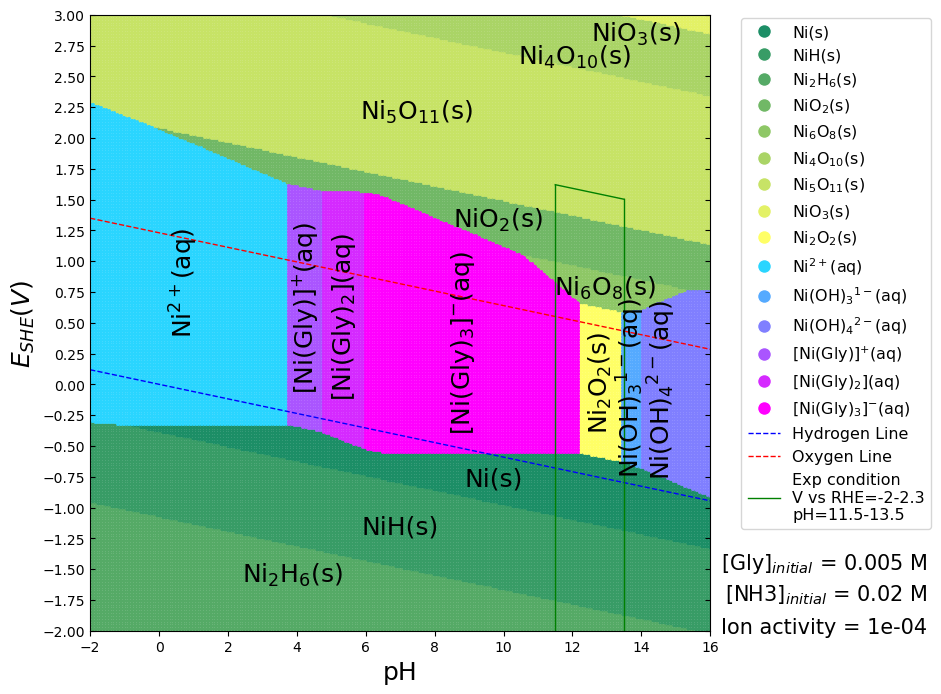
\includegraphics[width=\textwidth]{Figures/pourbaix_diagrams/Ni-NH3-H2O_activity=1e-04_[NH3]=0.02M_[Gly]=0.005M_[CN]=0.png}
%         \par\medskip
%     \end{subfigure}
%     % Subfigure (b)
%     \begin{subfigure}[b]{0.3\textwidth}
%         \subcaption{}\label{fig:Au_Pourbaix_NH3_Gly}
%         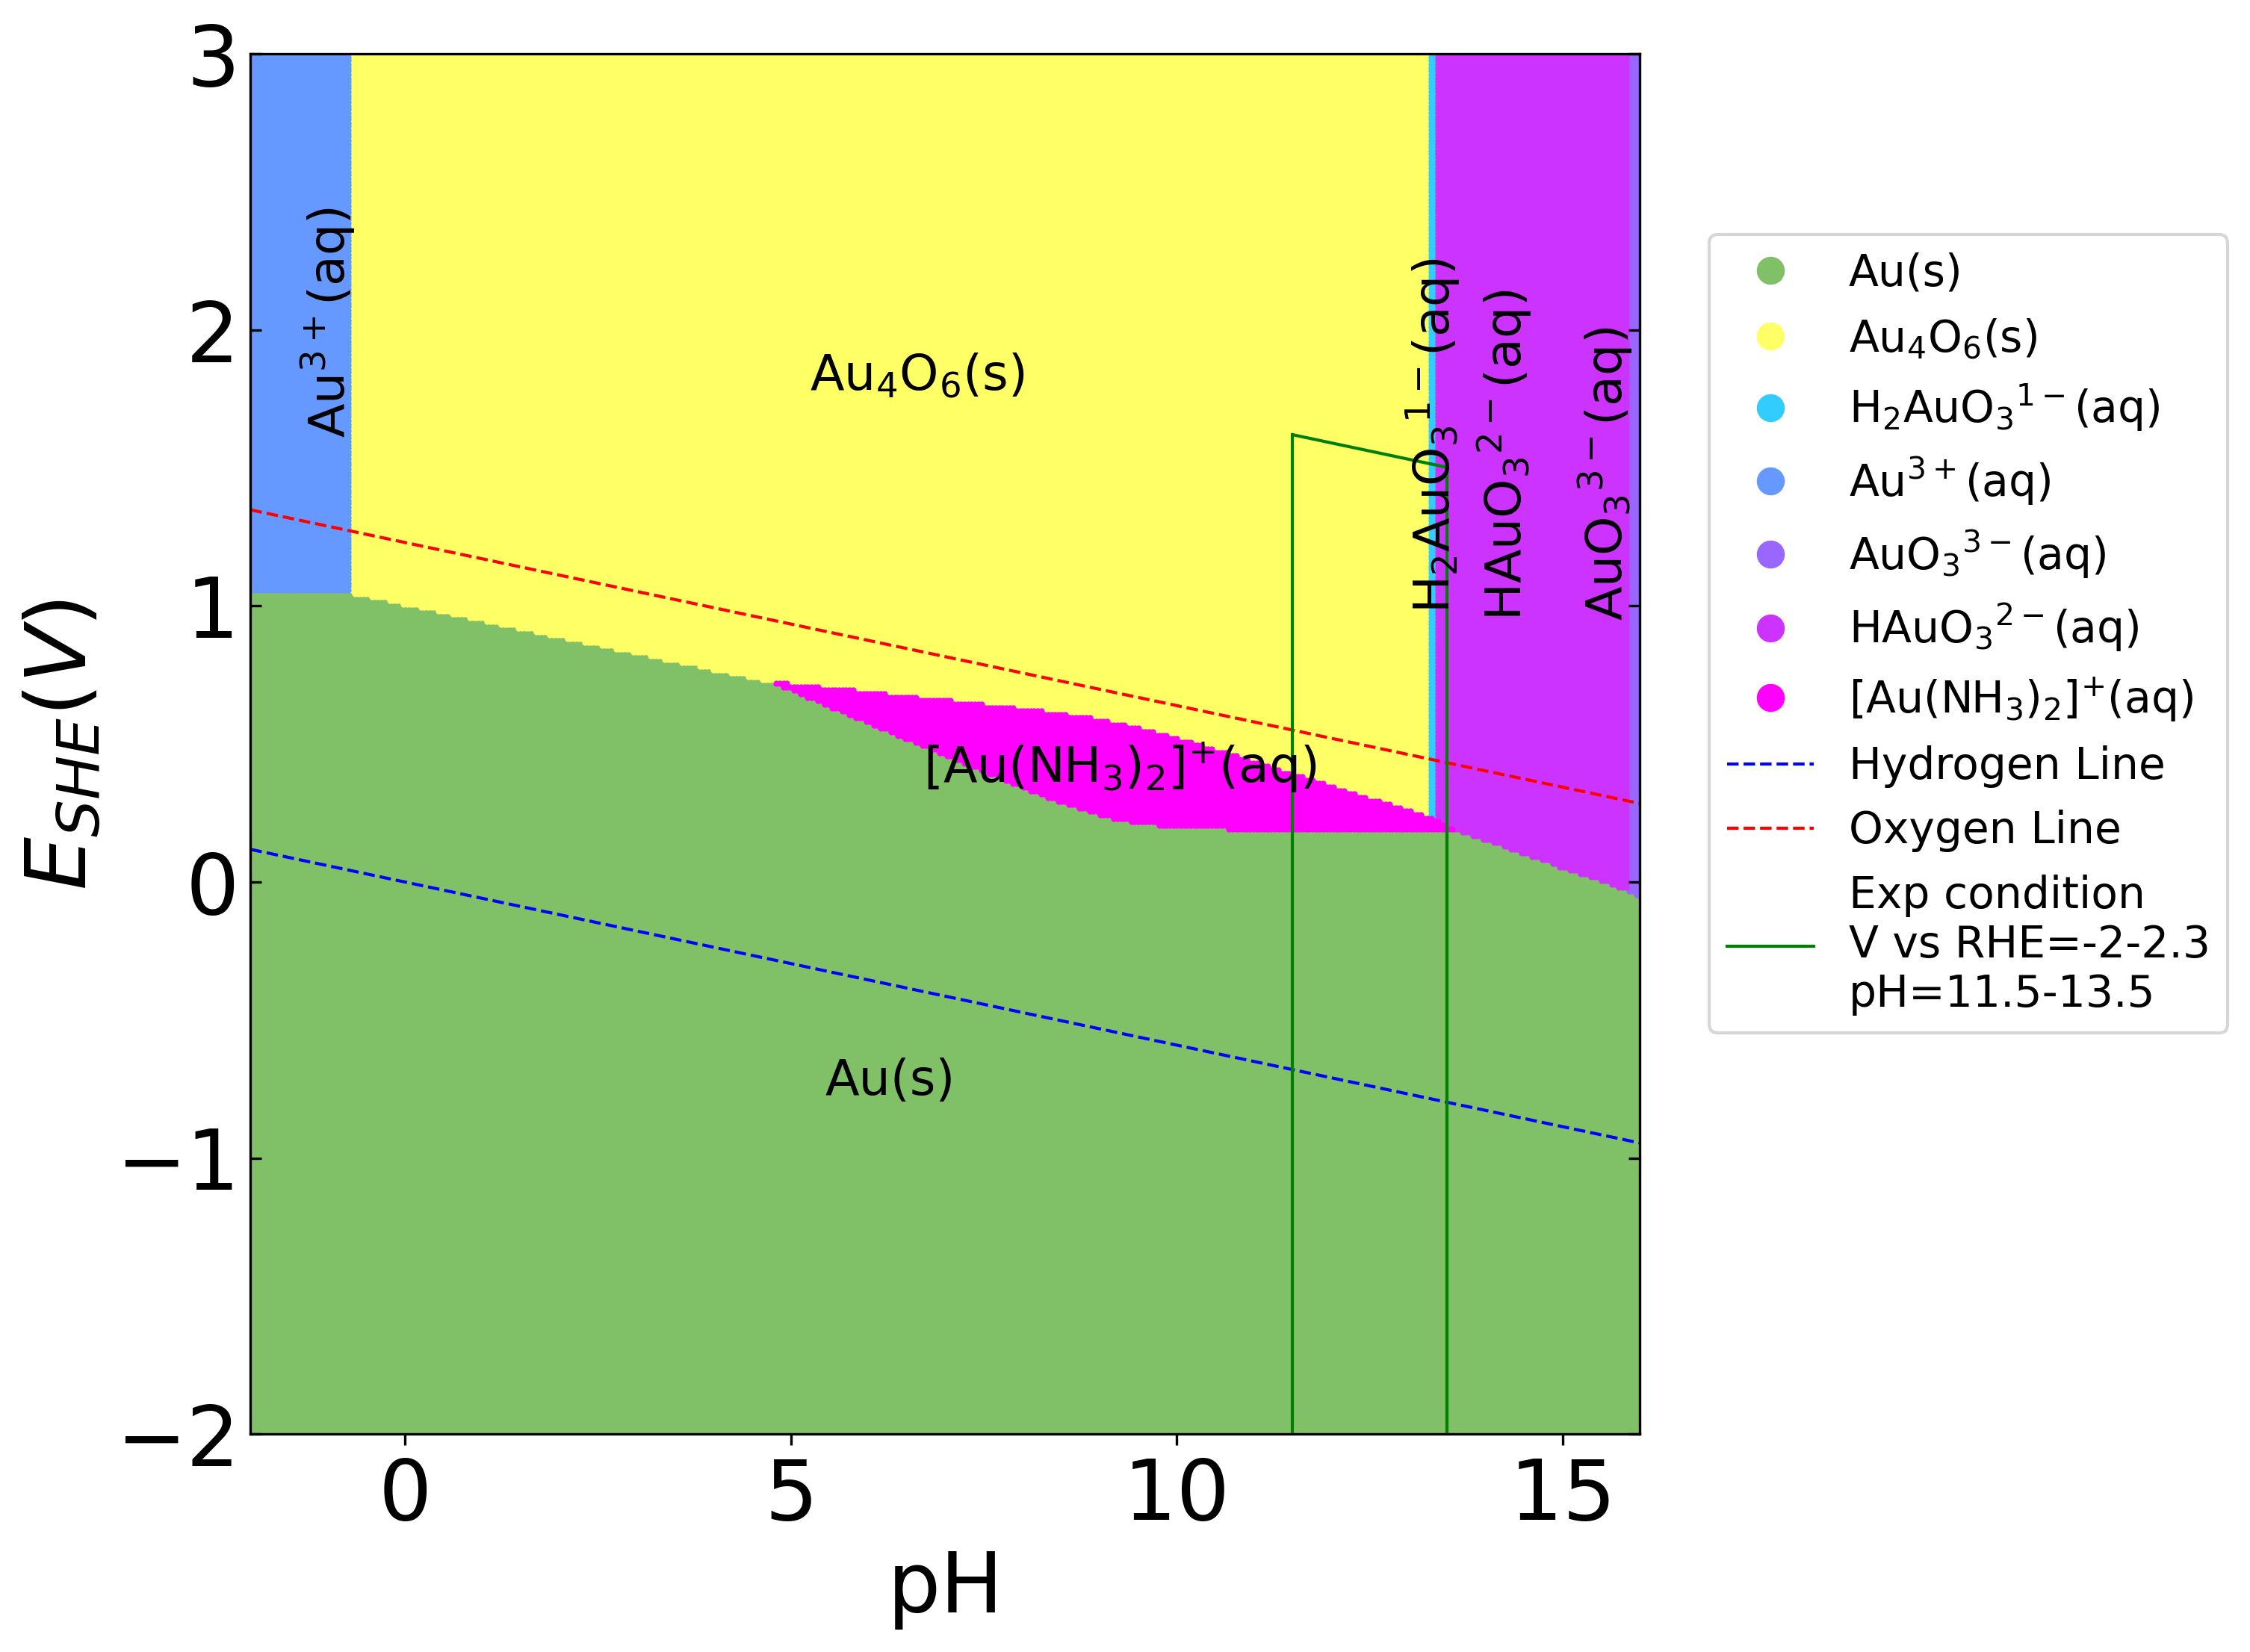
\includegraphics[width=\textwidth]{Figures/pourbaix_diagrams/Au-NH3-H2O_activity=1e-04_[NH3]=0.02M_[Gly]=0.005M_[CN]=0.png}
%         \par\medskip
%     \end{subfigure}
%     % Subfigure (c)
%     \begin{subfigure}[b]{0.3\textwidth}
%         \subcaption{}\label{fig:Cu_Pourbaix_NH3_Gly}
%         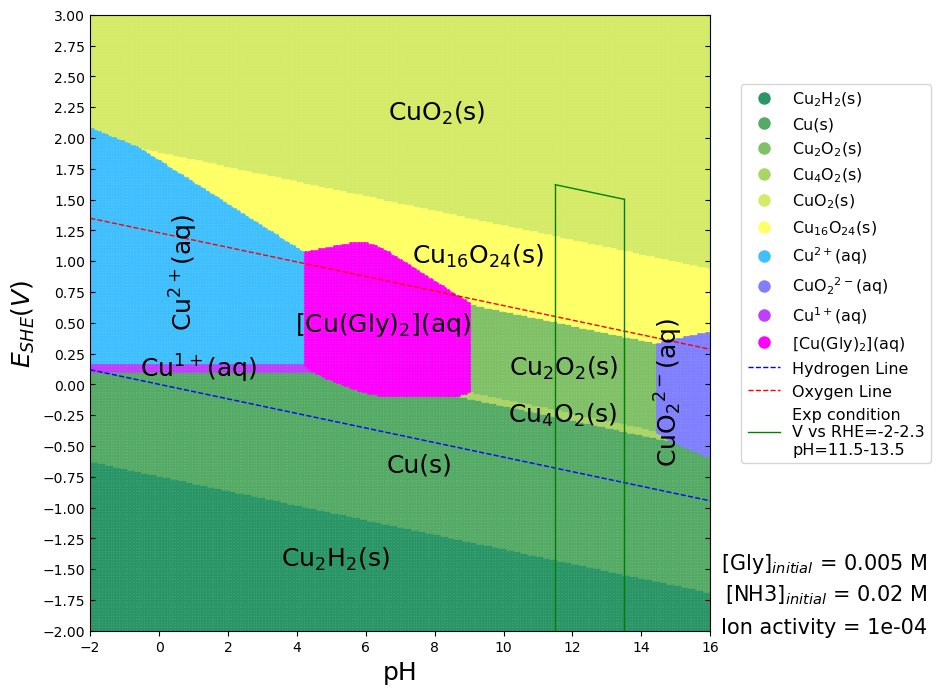
\includegraphics[width=\textwidth]{Figures/pourbaix_diagrams/Cu-NH3-H2O_activity=1e-04_[NH3]=0.02M_[Gly]=0.005M_[CN]=0.png}
%         \par\medskip   
%     \end{subfigure}
%     % Subfigure (d)
%     \begin{subfigure}[b]{0.3\textwidth}
%         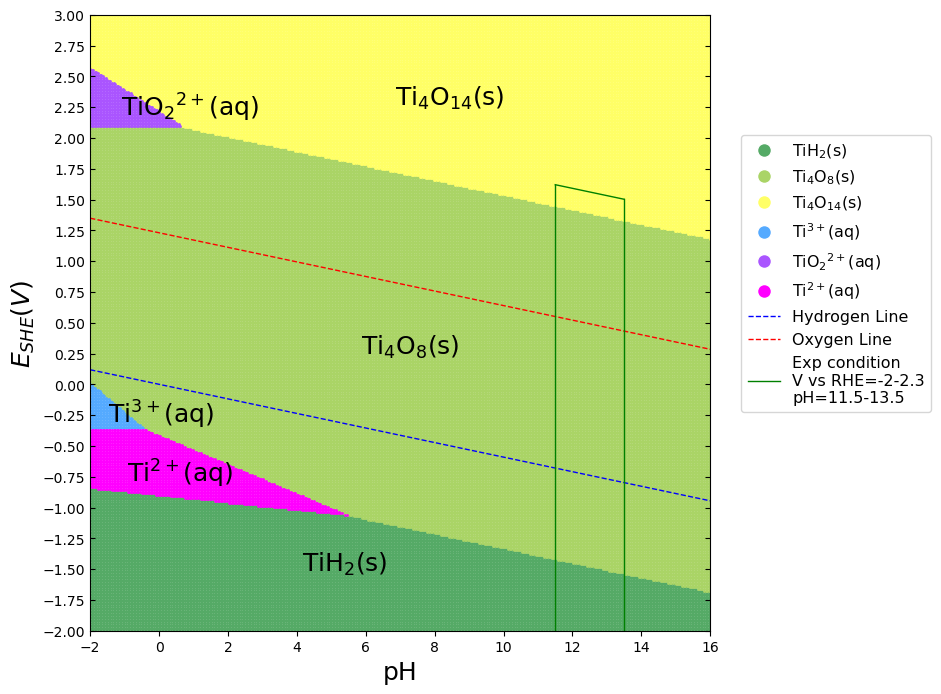
\includegraphics[width=\textwidth]{Figures/pourbaix_diagrams/Ti-NH3-H2O_activity=1e-04_[NH3]=0.02M_[Gly]=0.005M_[CN]=0.png}
%         \subcaption{}\label{fig:Ti_Pourbaix_NH3_Gly}
%     \end{subfigure}
%     % Subfigure (e)
%     \begin{subfigure}[b]{0.3\textwidth}
%         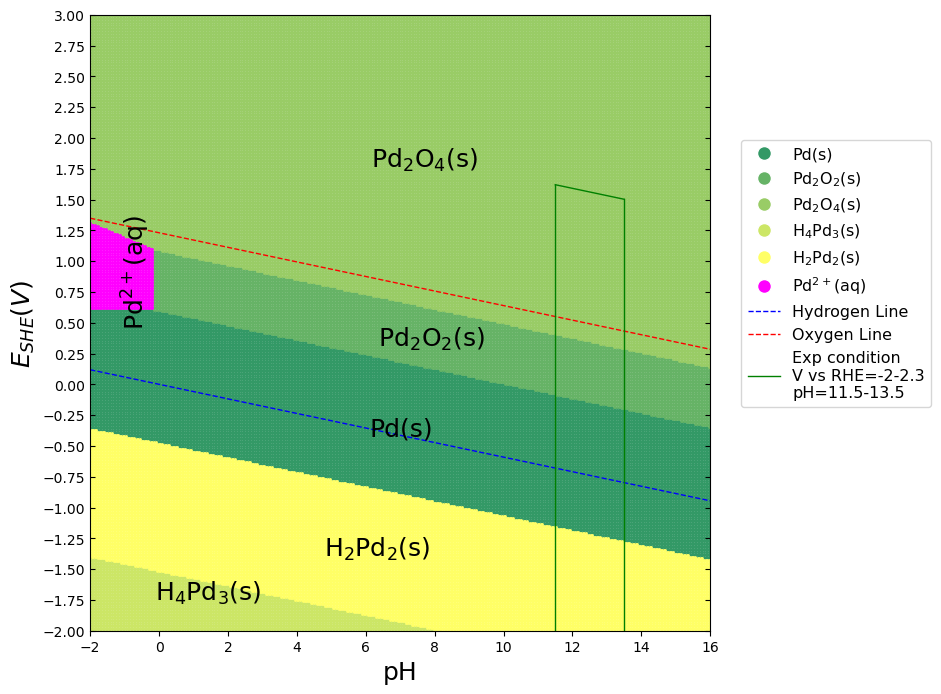
\includegraphics[width=\textwidth]{Figures/pourbaix_diagrams/Pd-NH3-H2O_activity=1e-04_[NH3]=0.02M_[Gly]=0.005M_[CN]=0.png}
%         \subcaption{}\label{fig:Pd_Pourbaix_NH3_Gly}
%     \end{subfigure}
%     % Subfigure (f)
%     \begin{subfigure}[b]{0.3\textwidth}
%         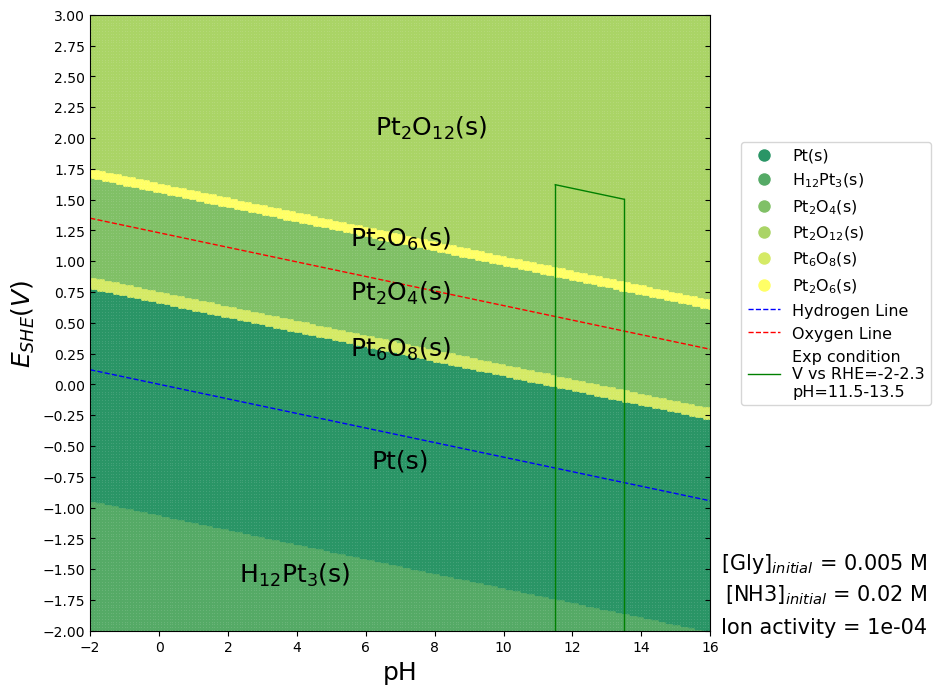
\includegraphics[width=\textwidth]{Figures/pourbaix_diagrams/Pt-NH3-H2O_activity=1e-04_[NH3]=0.02M_[Gly]=0.005M_[CN]=0.png}
%         \subcaption{}\label{fig:Pt_Pourbaix_NH3_Gly}
%     \end{subfigure}
%     \caption{Pourbaix diagrams for different metals at $[NH_3]_{initial}= 0.02M$, $[Gly]_{initial}=0.005M$. Green box indicates experimental condition at applied potential vs RHE = -2 to 2 V, pH = 11.5 to 13.5.}
%     \label{fig:Pourbaix_NH3_Gly}
% \end{figure}
%%%%%%%%%%%%%%%%%%%%%%%%%%%%%%%%% H2O only %%%%%%%%%%%%%%%%%%%%%%%%%%%%%%%%%

% \begin{figure}[htbp]
%     \centering
%     % Subfigure (a)
%     \begin{subfigure}[b]{0.3\textwidth}
%         \subcaption{}\label{fig:Ni_Pourbaix_H2O}
%         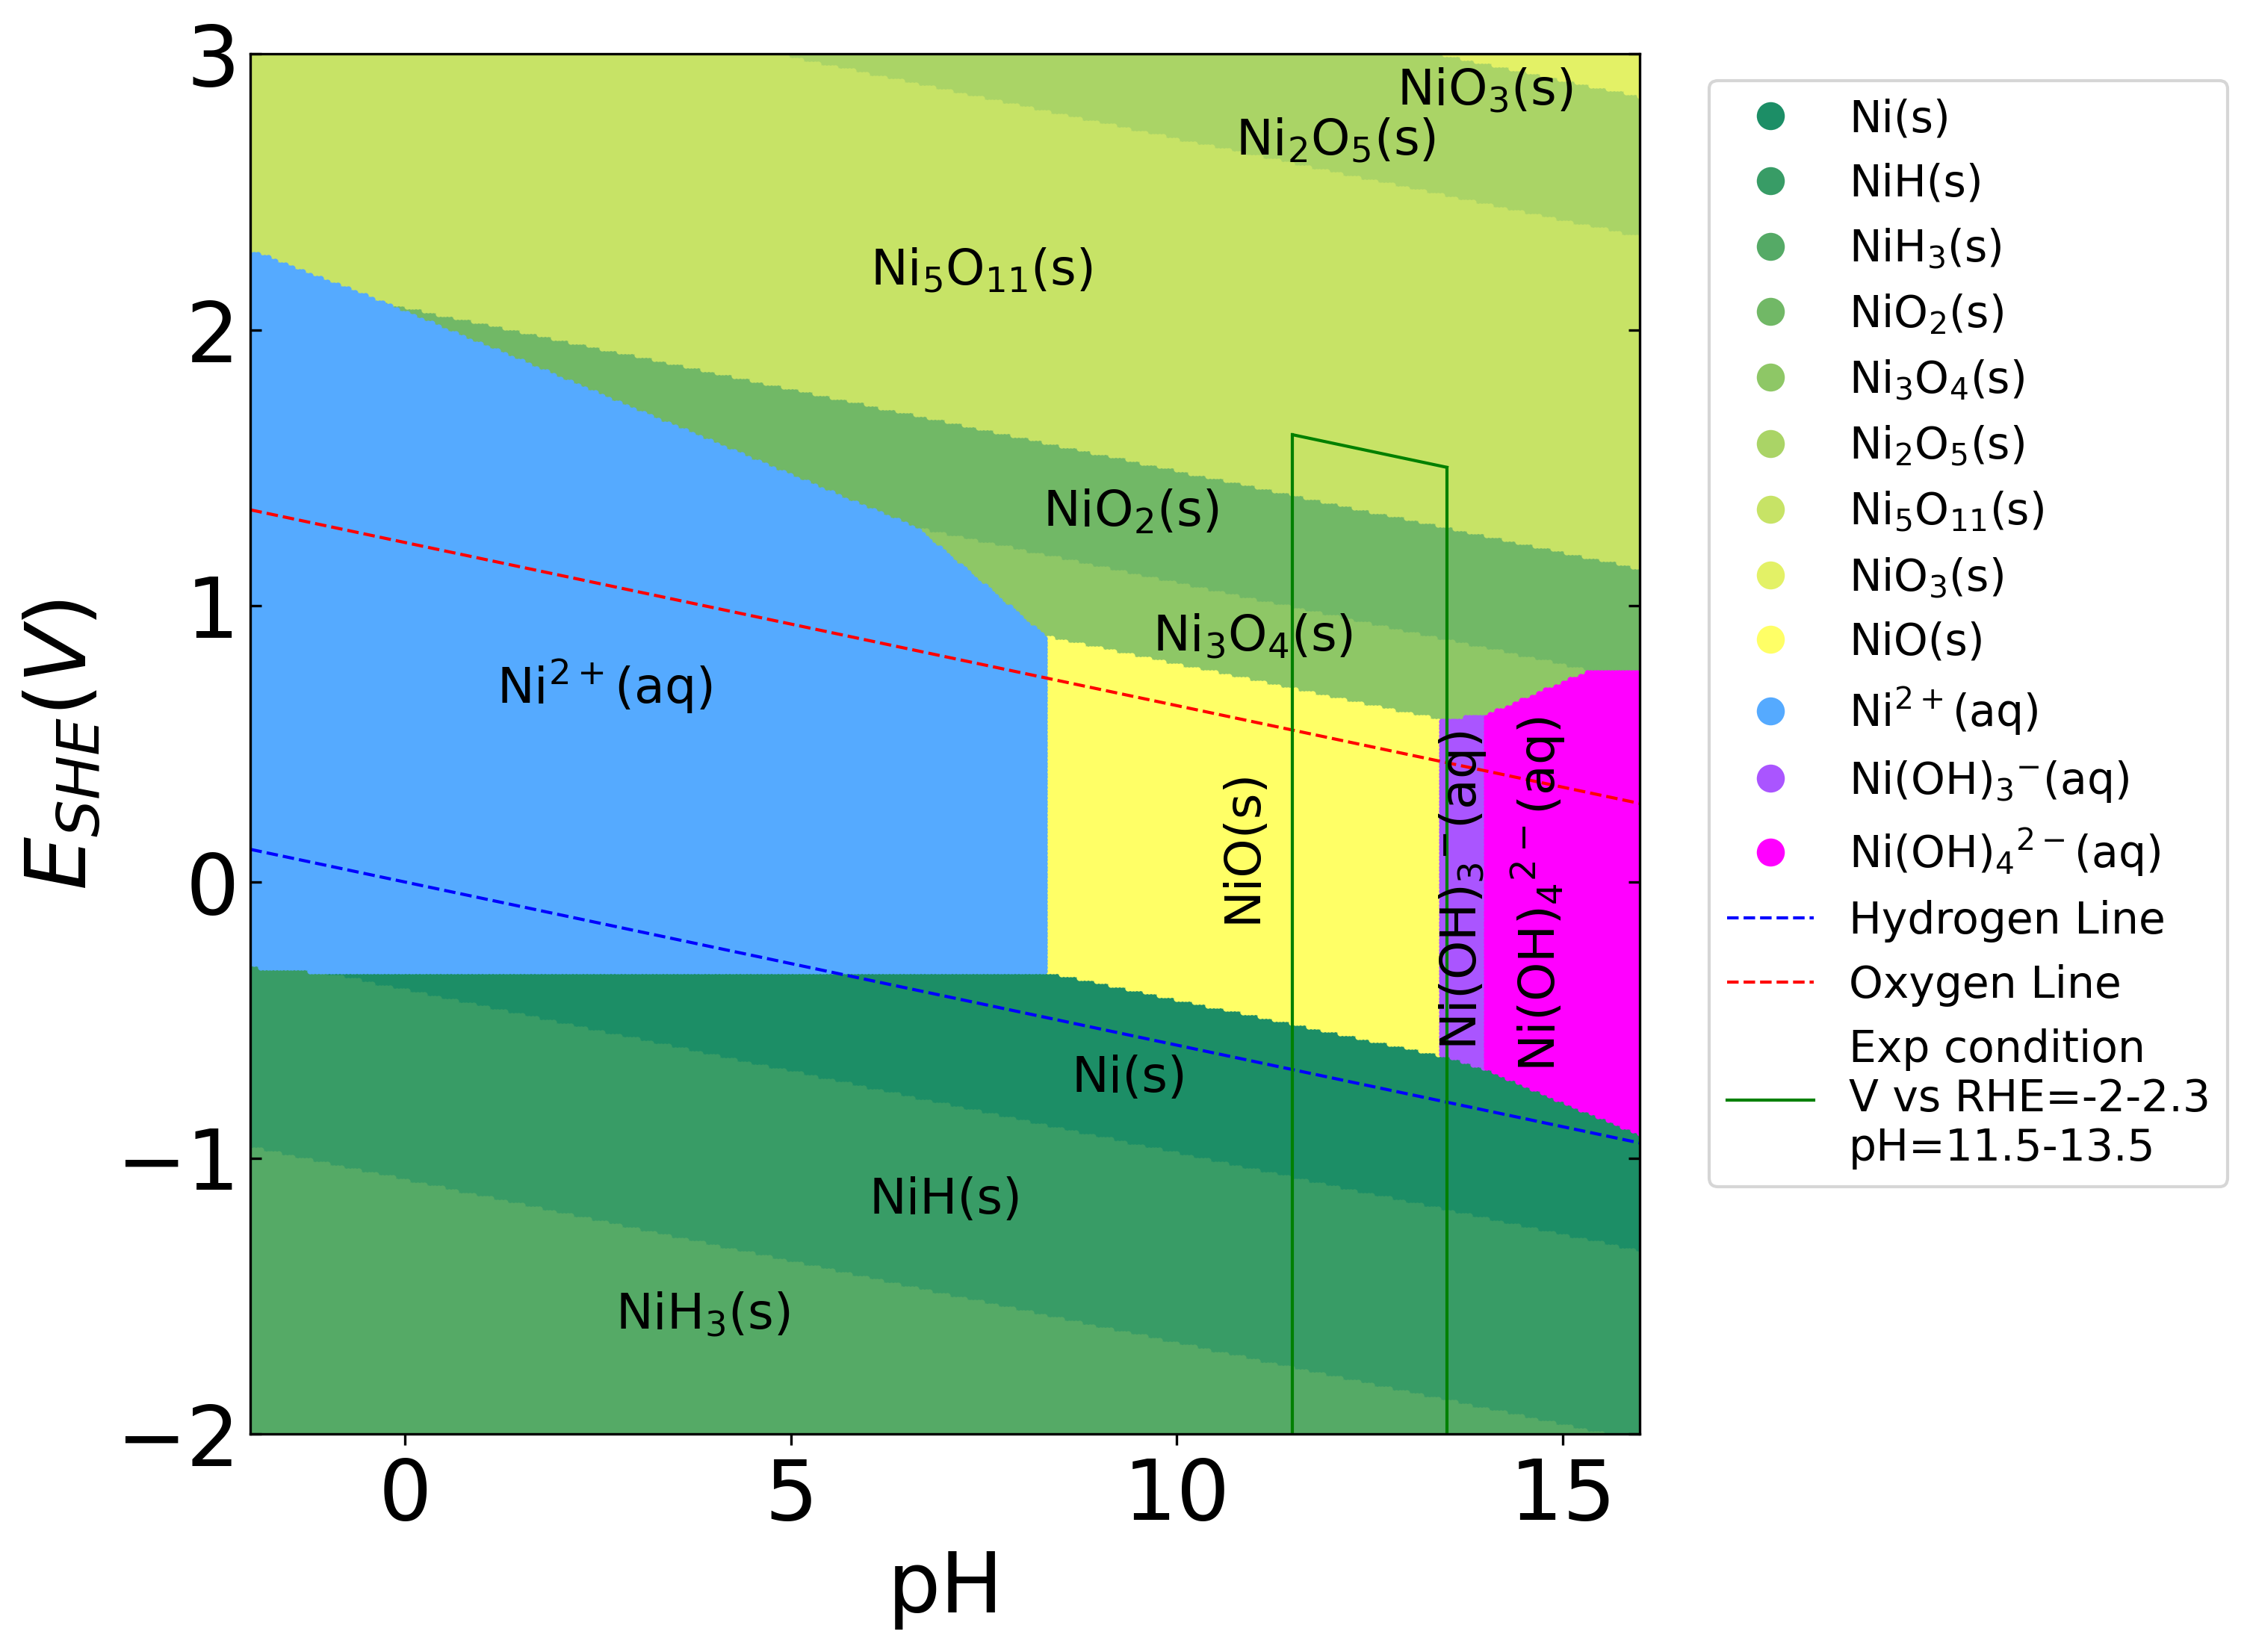
\includegraphics[width=\textwidth]{Figures/pourbaix_diagrams/Ni-NH3-H2O_activity=1e-04_[NH3]=0M_[Gly]=0M_[CN]=0.png}
%         \par\medskip
%     \end{subfigure}
%     % Subfigure (b)
%     \begin{subfigure}[b]{0.3\textwidth}
%         \subcaption{}\label{fig:Au_Pourbaix_H2O}
%         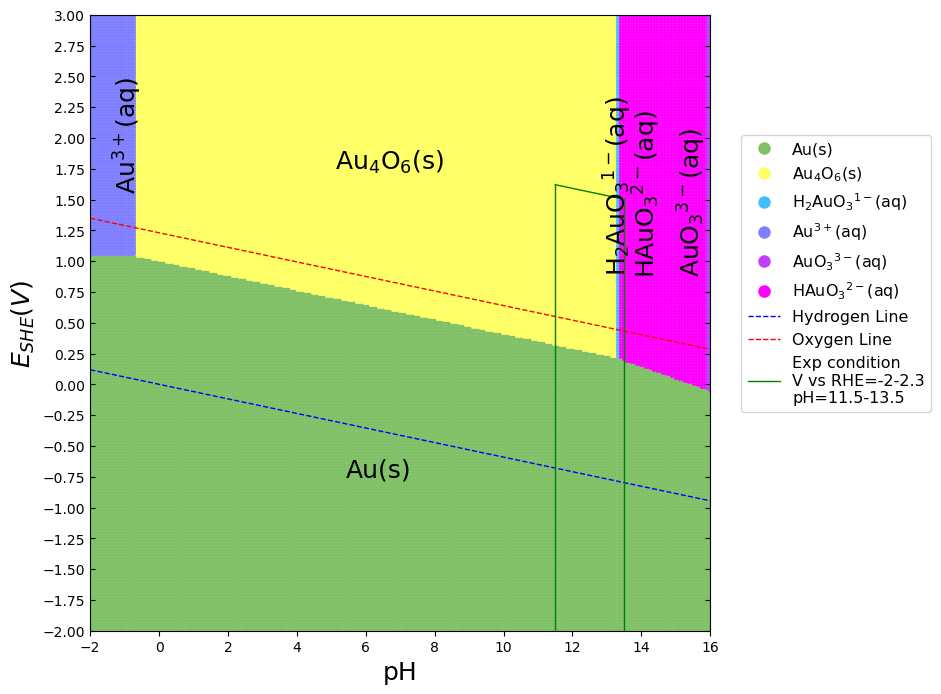
\includegraphics[width=\textwidth]{Figures/pourbaix_diagrams/Au-NH3-H2O_activity=1e-04_[NH3]=0M_[Gly]=0M_[CN]=0.png}
%         \par\medskip
%     \end{subfigure}
%     % Subfigure (c)
%     \begin{subfigure}[b]{0.3\textwidth}
%         \subcaption{}\label{fig:Cu_Pourbaix_H2O}
%         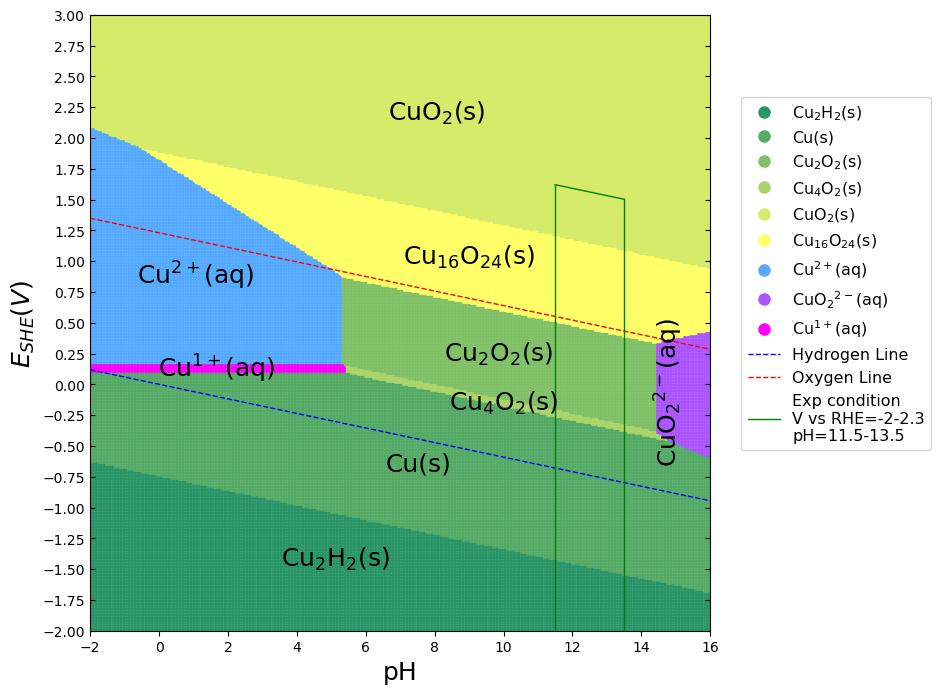
\includegraphics[width=\textwidth]{Figures/pourbaix_diagrams/Cu-NH3-H2O_activity=1e-04_[NH3]=0M_[Gly]=0M_[CN]=0.png}
%         \par\medskip   
%     \end{subfigure}
%     % Subfigure (d)
%     \begin{subfigure}[b]{0.3\textwidth}
%         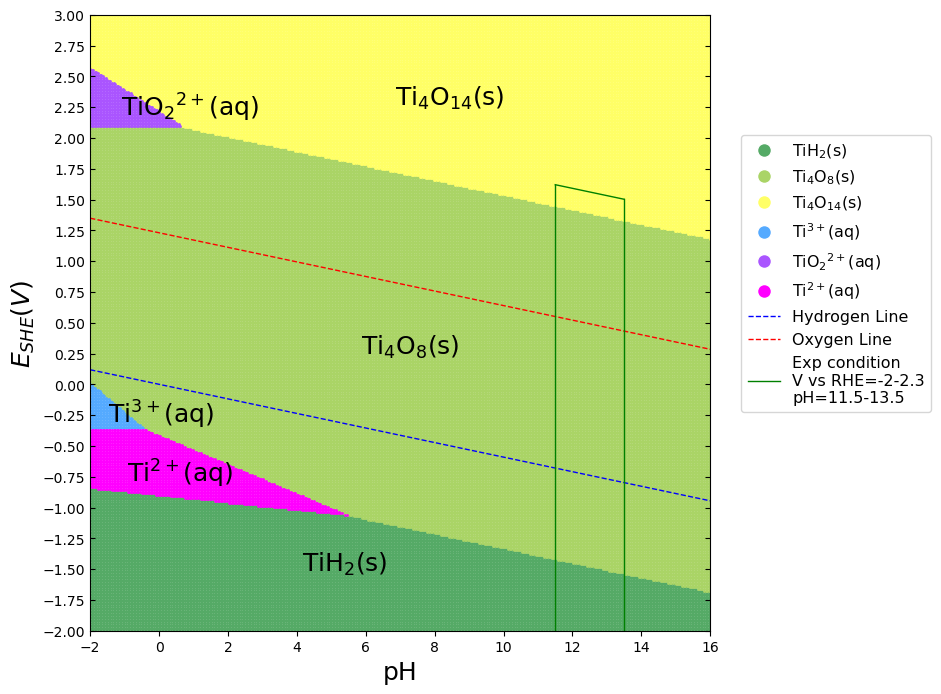
\includegraphics[width=\textwidth]{Figures/pourbaix_diagrams/Ti-NH3-H2O_activity=1e-04_[NH3]=0M_[Gly]=0M_[CN]=0.png}
%         \subcaption{}\label{fig:Ti_Pourbaix_H2O}
%     \end{subfigure}
%     % Subfigure (e)
%     \begin{subfigure}[b]{0.3\textwidth}
%         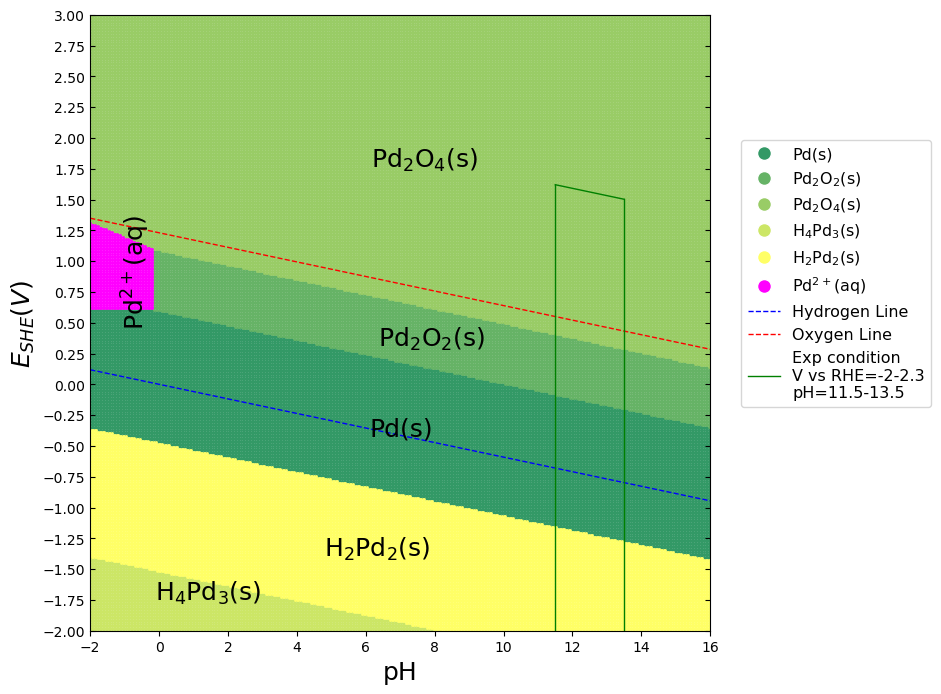
\includegraphics[width=\textwidth]{Figures/pourbaix_diagrams/Pd-NH3-H2O_activity=1e-04_[NH3]=0M_[Gly]=0M_[CN]=0.png}
%         \subcaption{}\label{fig:Pd_Pourbaix_H2O}
%     \end{subfigure}
%     % Subfigure (f)
%     \begin{subfigure}[b]{0.3\textwidth}
%         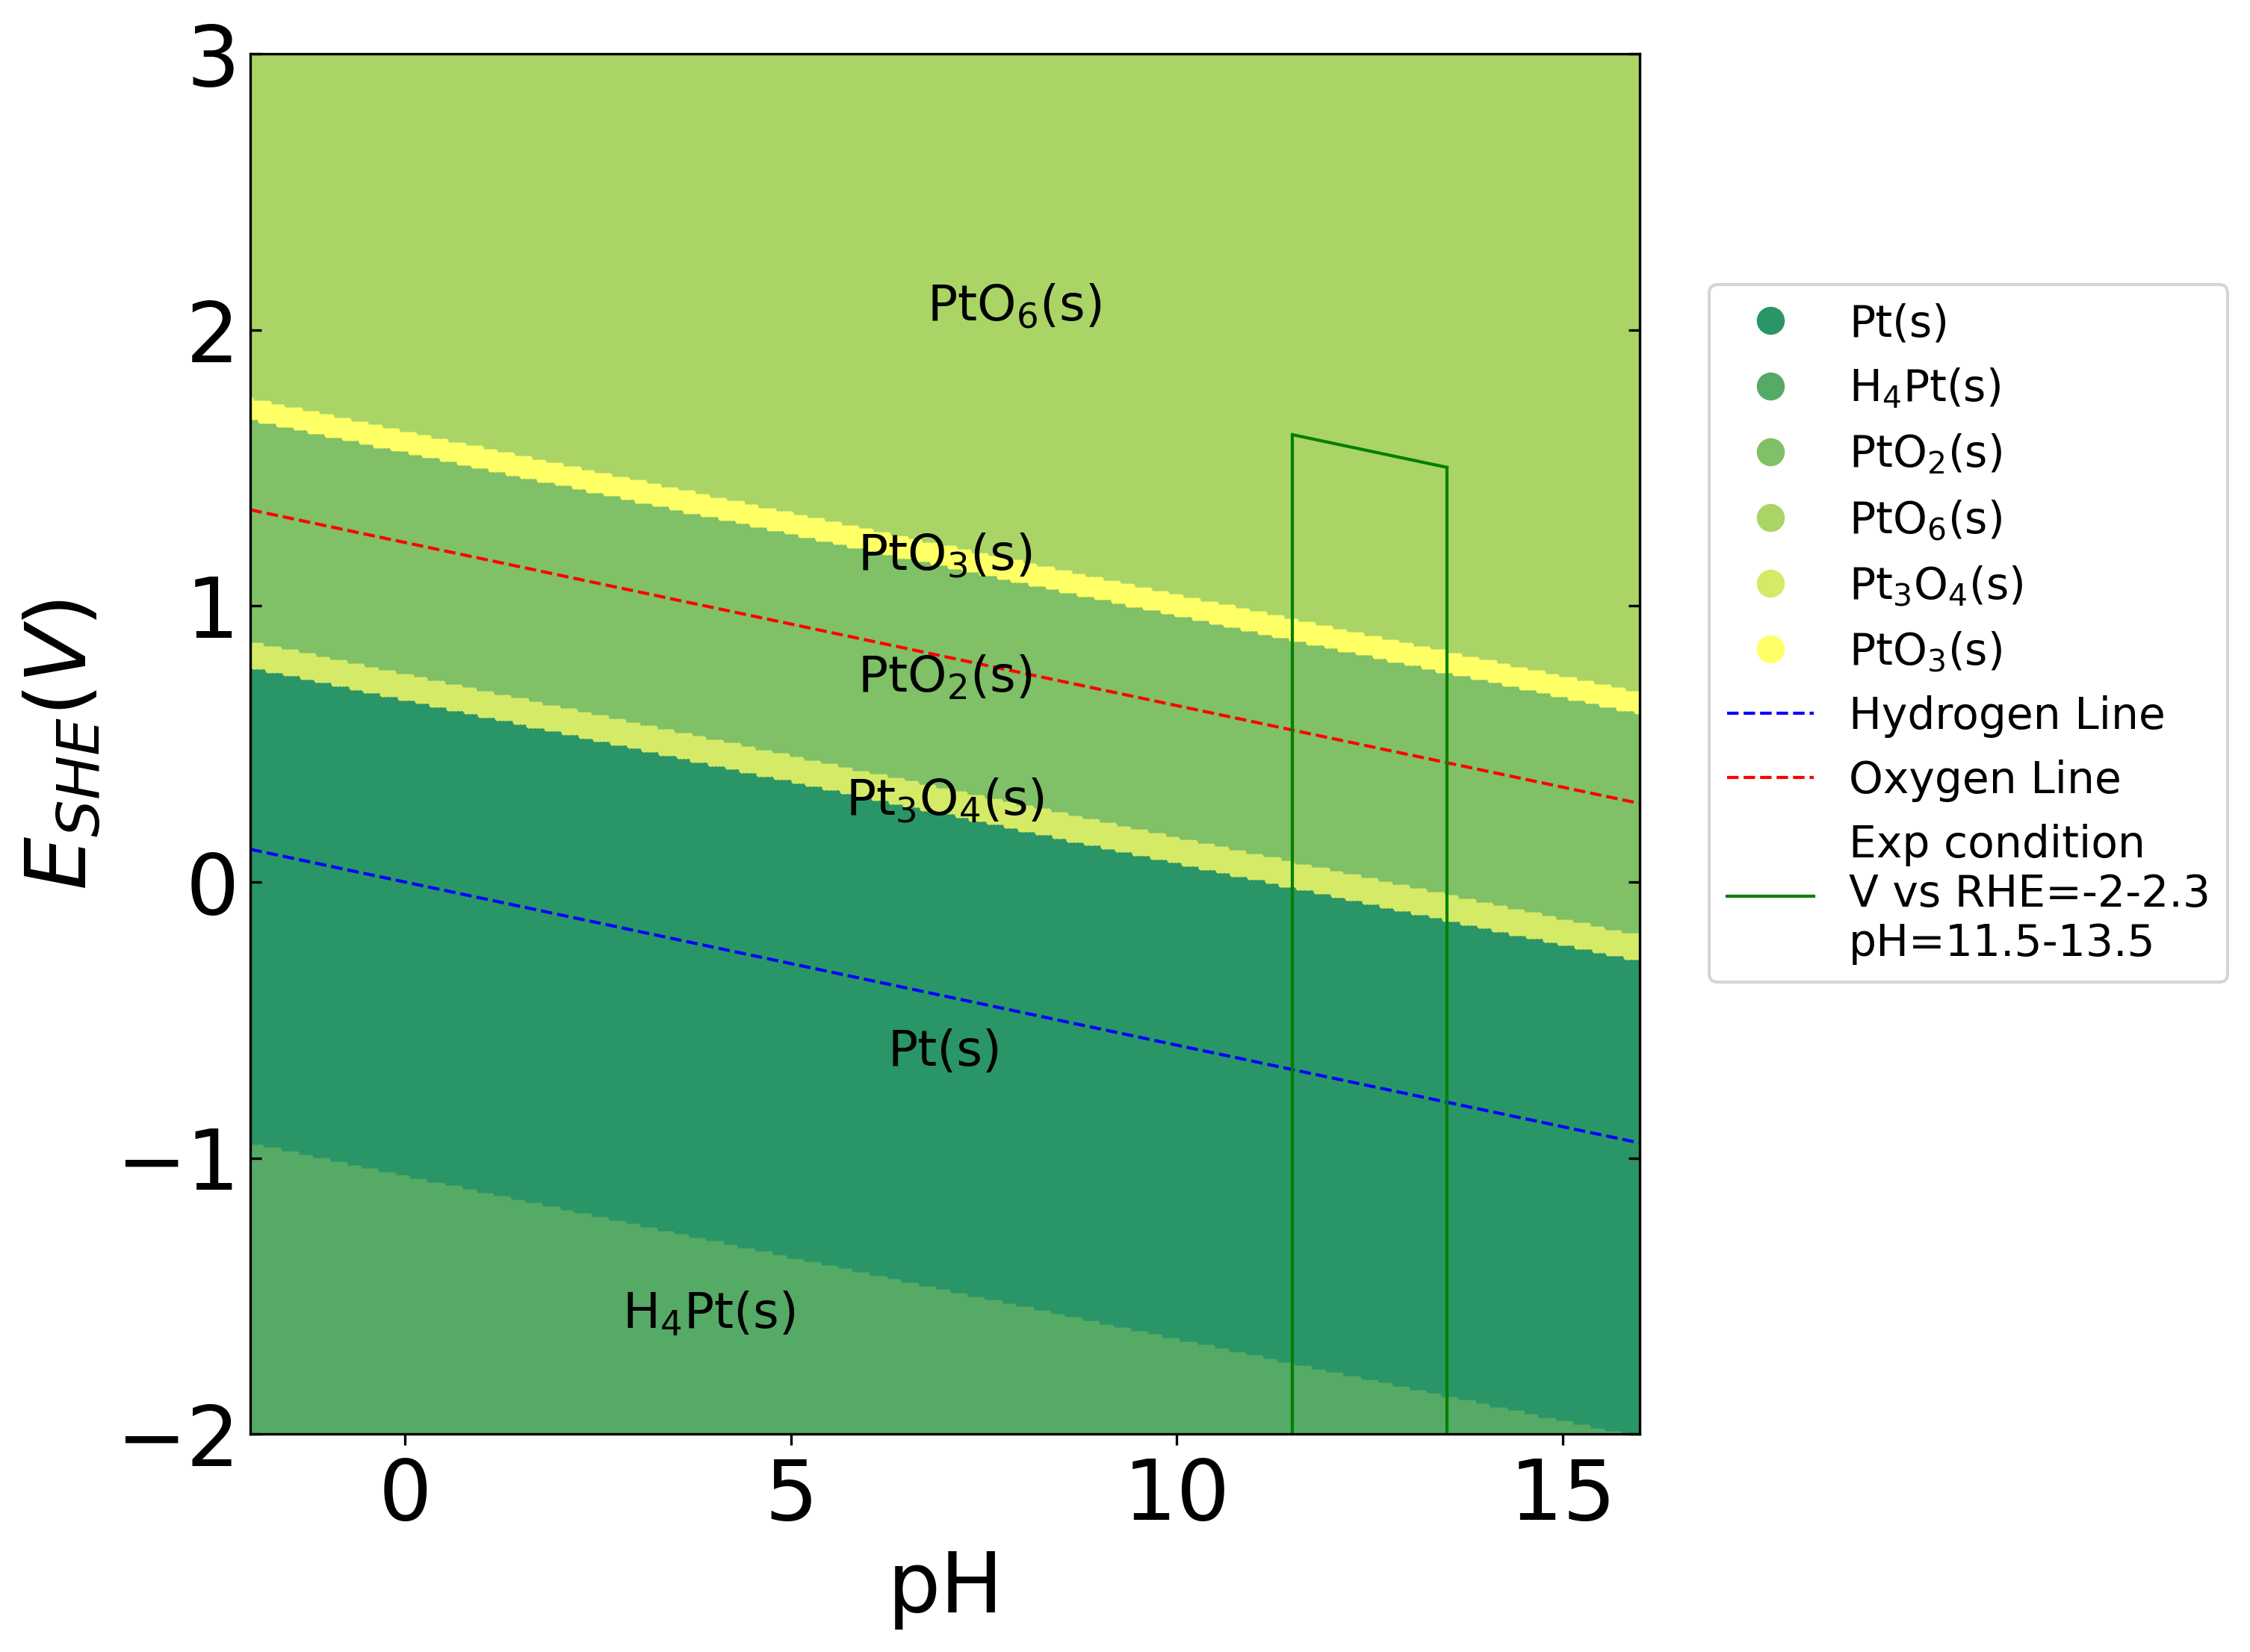
\includegraphics[width=\textwidth]{Figures/pourbaix_diagrams/Pt-NH3-H2O_activity=1e-04_[NH3]=0M_[Gly]=0M_[CN]=0.png}
%         \subcaption{}\label{fig:Pt_Pourbaix_H2O}
%     \end{subfigure}

%     \caption{Pourbaix diagrams for metal-\ce{H2O} systems. Green box indicates experimental condition at applied potential vs RHE = -2 to 2 V, pH = 11.5 to 13.5.}
%     \label{fig:Pourbaix_NH3_Gly}
% \end{figure}

%%%%%%%%%%%%%%%%%%%%%%%%%%%%%%%%% NH3, Gly and CN- %%%%%%%%%%%%%%%%%%%%%%%%%%%%%%%%%
% \begin{figure}[htbp]
%     \centering
%     % Subfigure (a)
%     \begin{subfigure}[b]{0.3\textwidth}
%         \subcaption{}\label{fig:Ni_Pourbaix_CN_CH3_Gly}
%         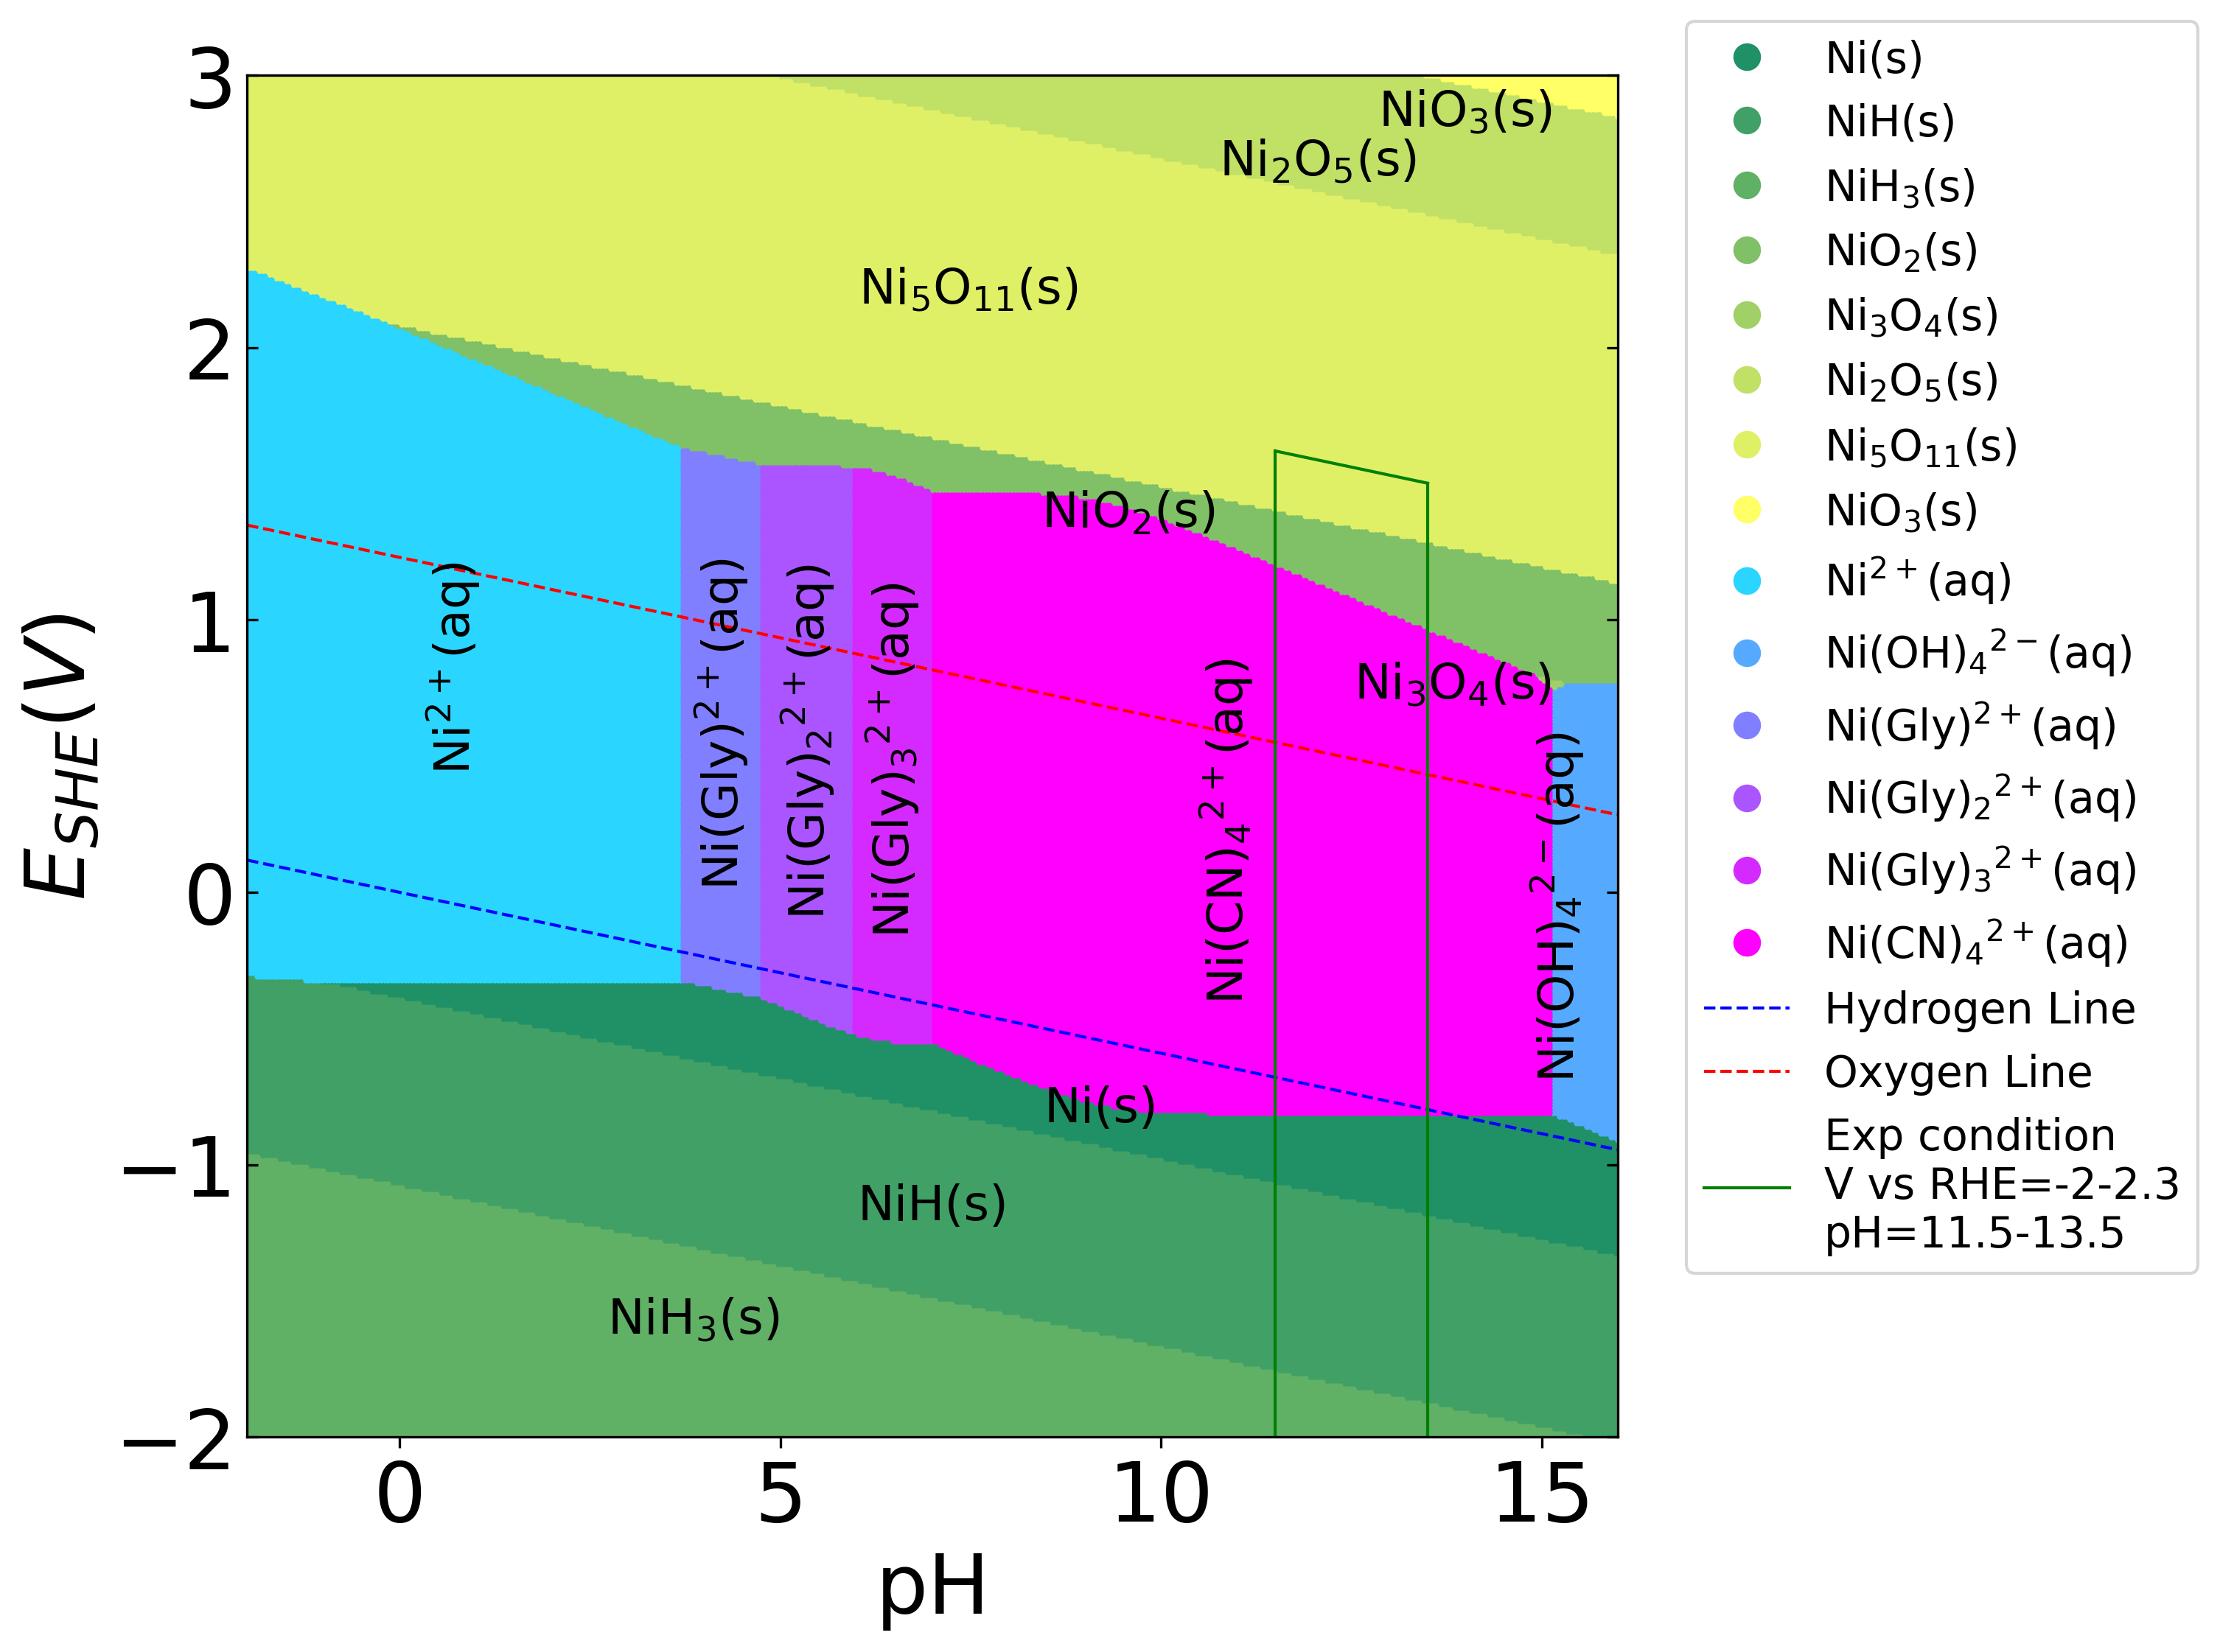
\includegraphics[width=\textwidth]{Figures/pourbaix_diagrams/Ni-NH3-H2O_activity=1e-04_[NH3]=0.02M_[Gly]=0.005M_[CN]=0.0001.png}
%         \par\medskip
%     \end{subfigure}
%     % Subfigure (b)
%     \begin{subfigure}[b]{0.3\textwidth}
%         \subcaption{}\label{fig:Au_Pourbaix_CN_CH3_Gly}
%         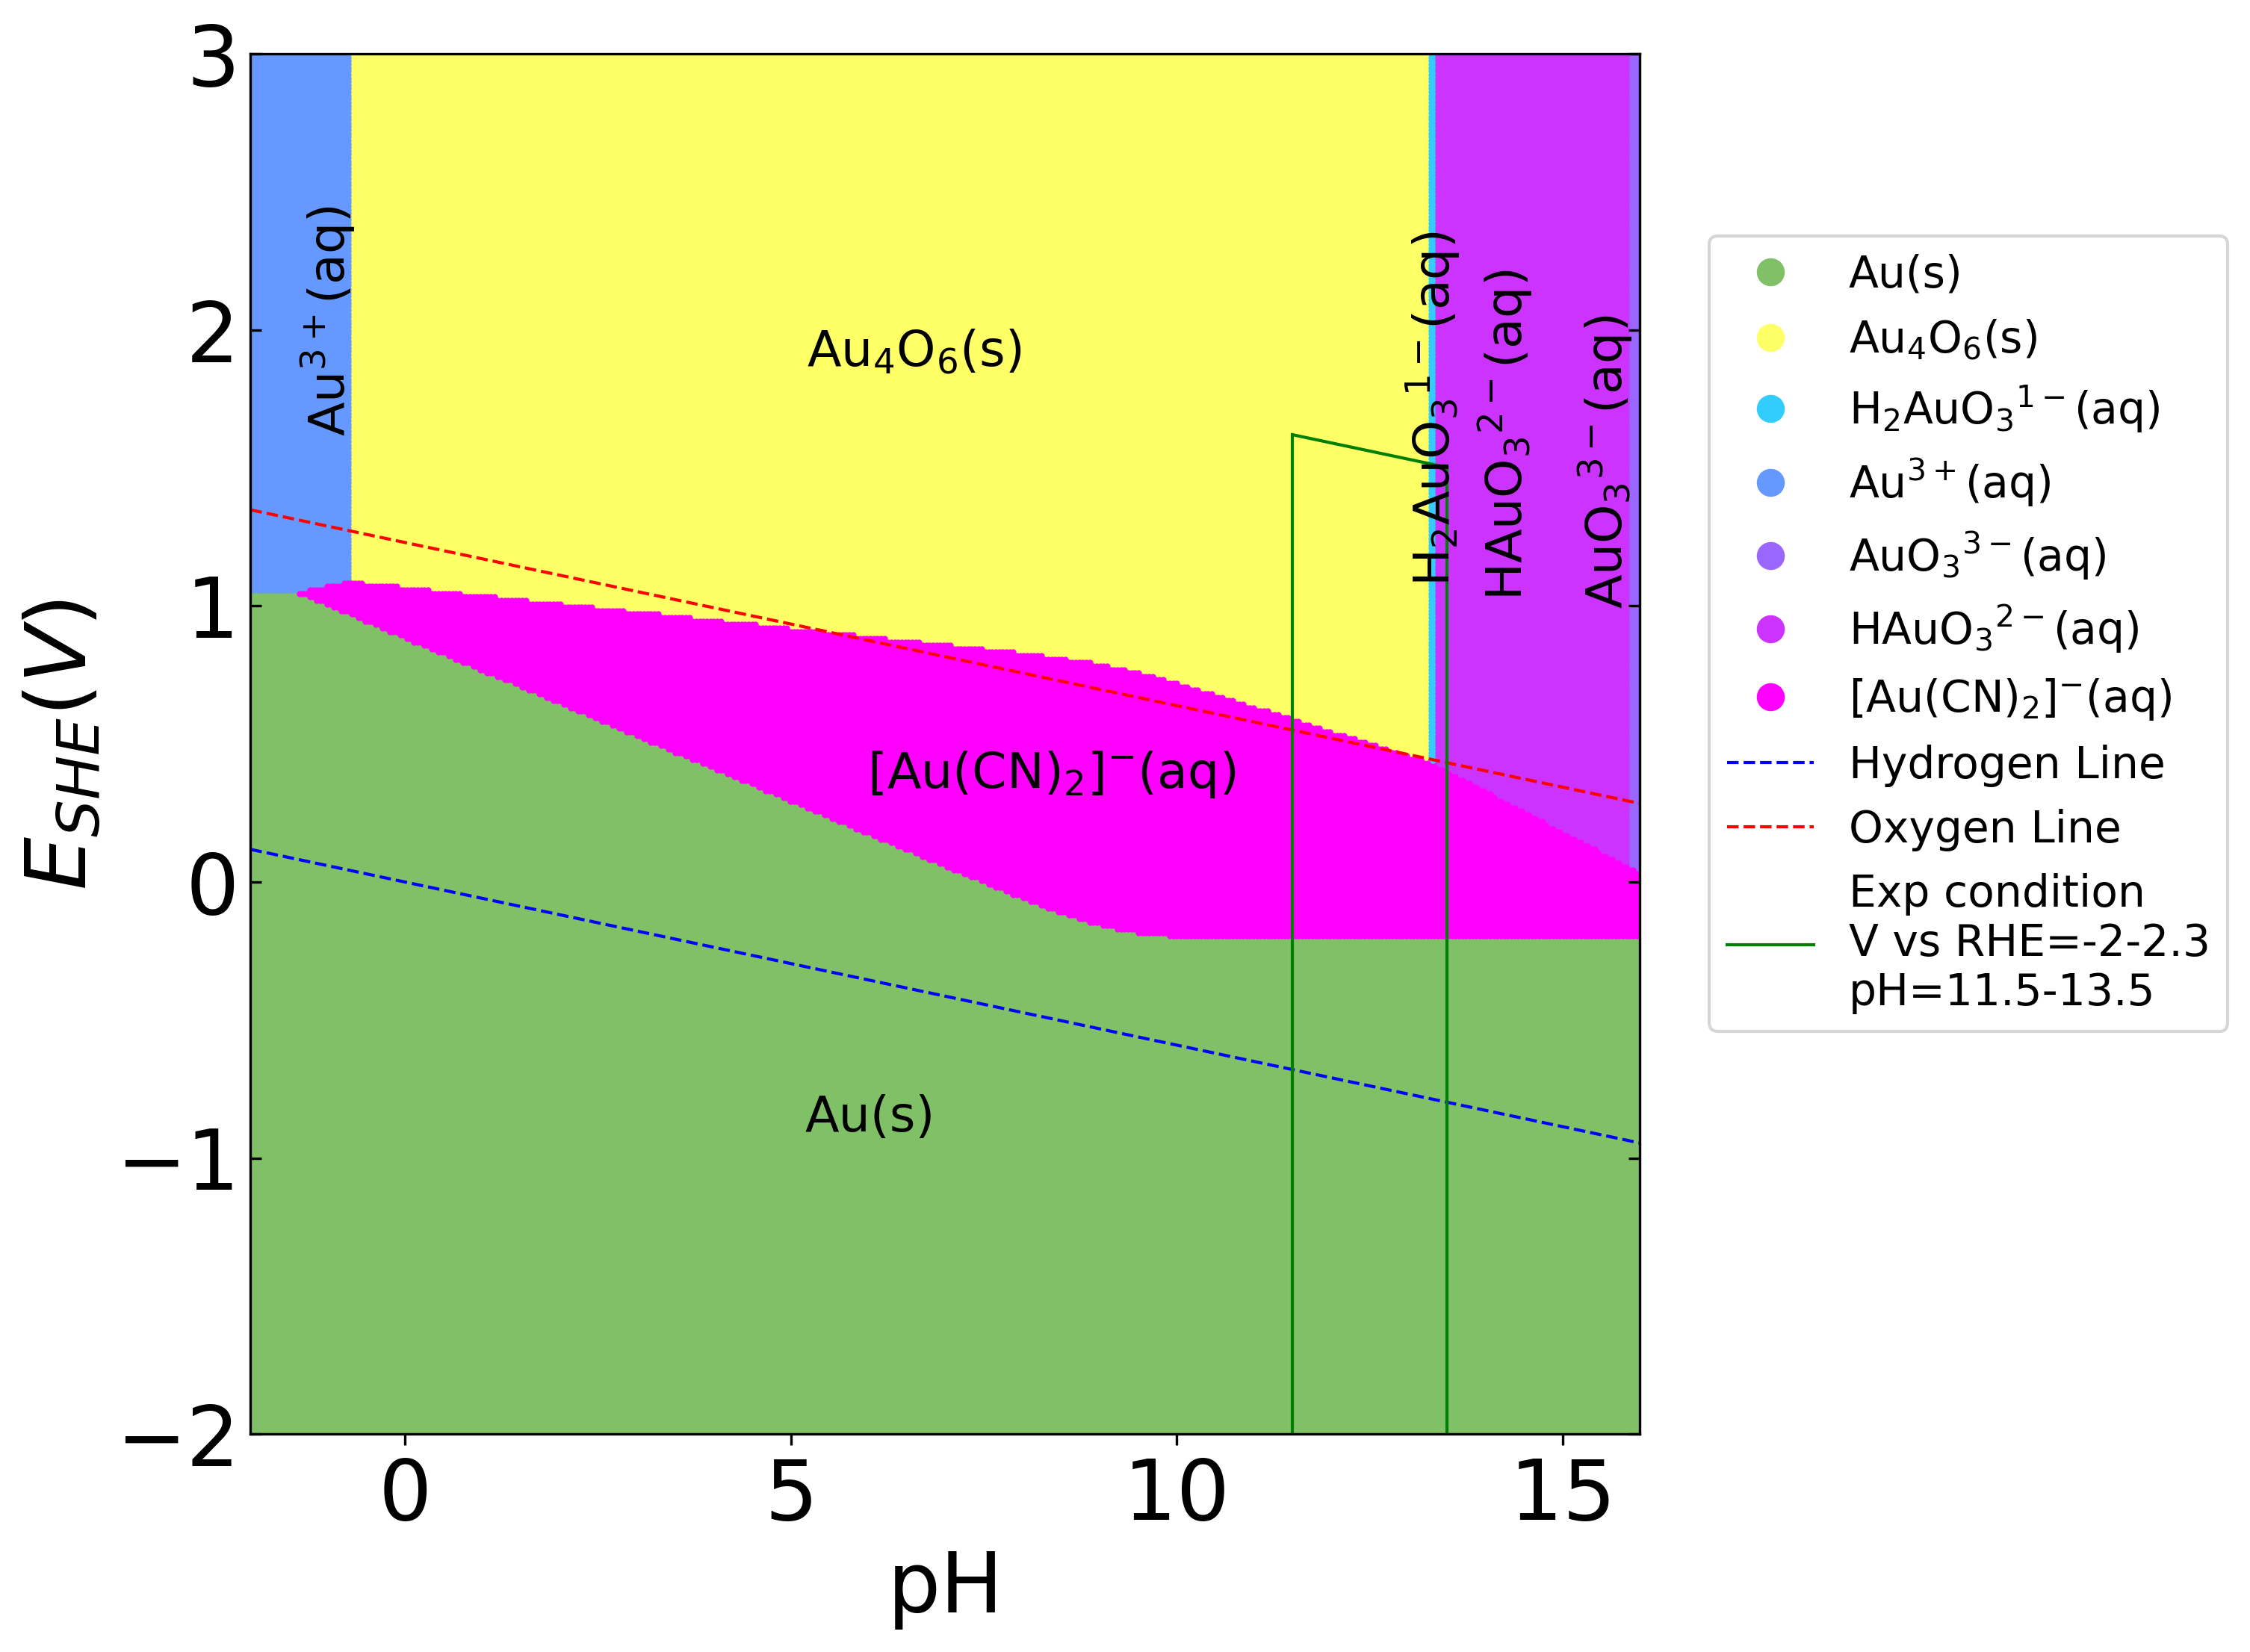
\includegraphics[width=\textwidth]{Figures/pourbaix_diagrams/Au-NH3-H2O_activity=1e-04_[NH3]=0.02M_[Gly]=0.005M_[CN]=0.0001.png}
%         \par\medskip
%     \end{subfigure}
%     % Subfigure (c)
%     \begin{subfigure}[b]{0.3\textwidth}
%         \subcaption{}\label{fig:Cu_Pourbaix_CN_CH3_Gly}
%         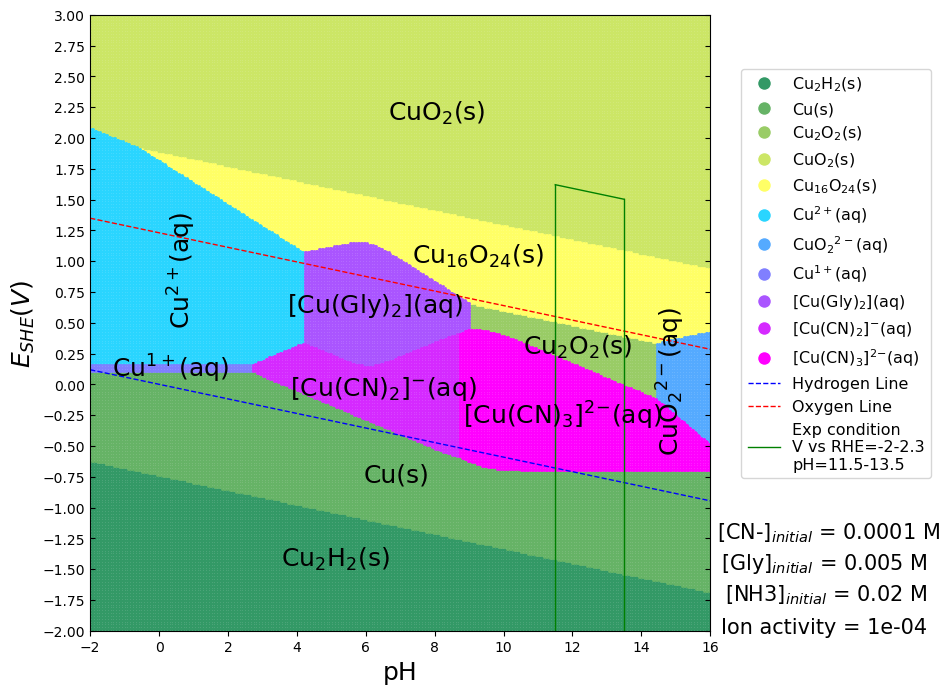
\includegraphics[width=\textwidth]{Figures/pourbaix_diagrams/Cu-NH3-H2O_activity=1e-04_[NH3]=0.02M_[Gly]=0.005M_[CN]=0.0001.png}
%         \par\medskip   
%     \end{subfigure}
%     % Subfigure (d)
%     \begin{subfigure}[b]{0.3\textwidth}
%         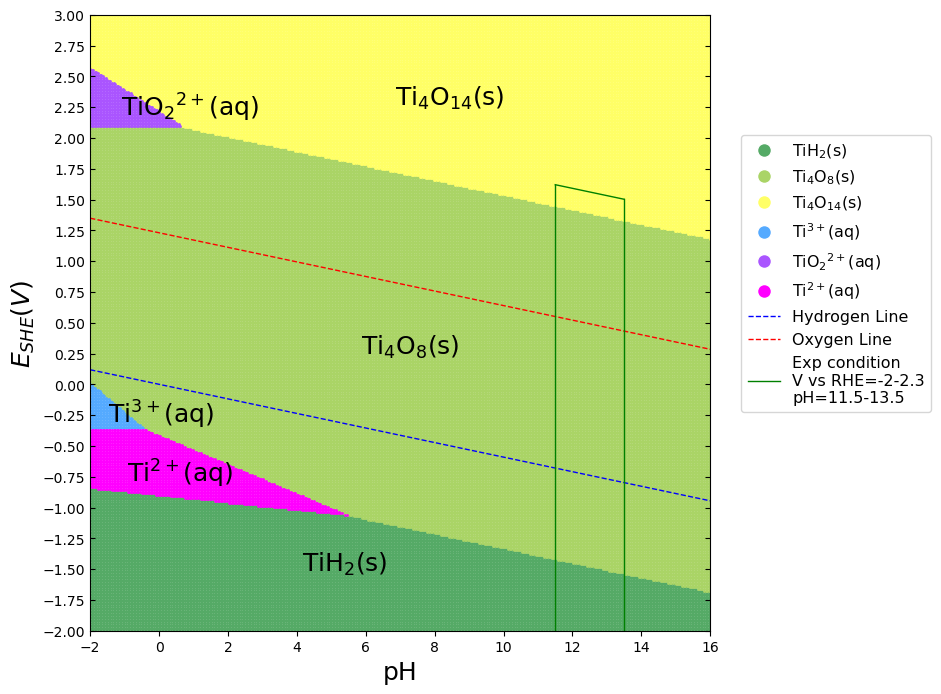
\includegraphics[width=\textwidth]{Figures/pourbaix_diagrams/Ti-NH3-H2O_activity=1e-04_[NH3]=0.02M_[Gly]=0.005M_[CN]=0.0001.png}
%         \subcaption{}\label{fig:Ti_Pourbaix_CN_CH3_Gly}
%     \end{subfigure}
%     % Subfigure (e)
%     \begin{subfigure}[b]{0.3\textwidth}
%         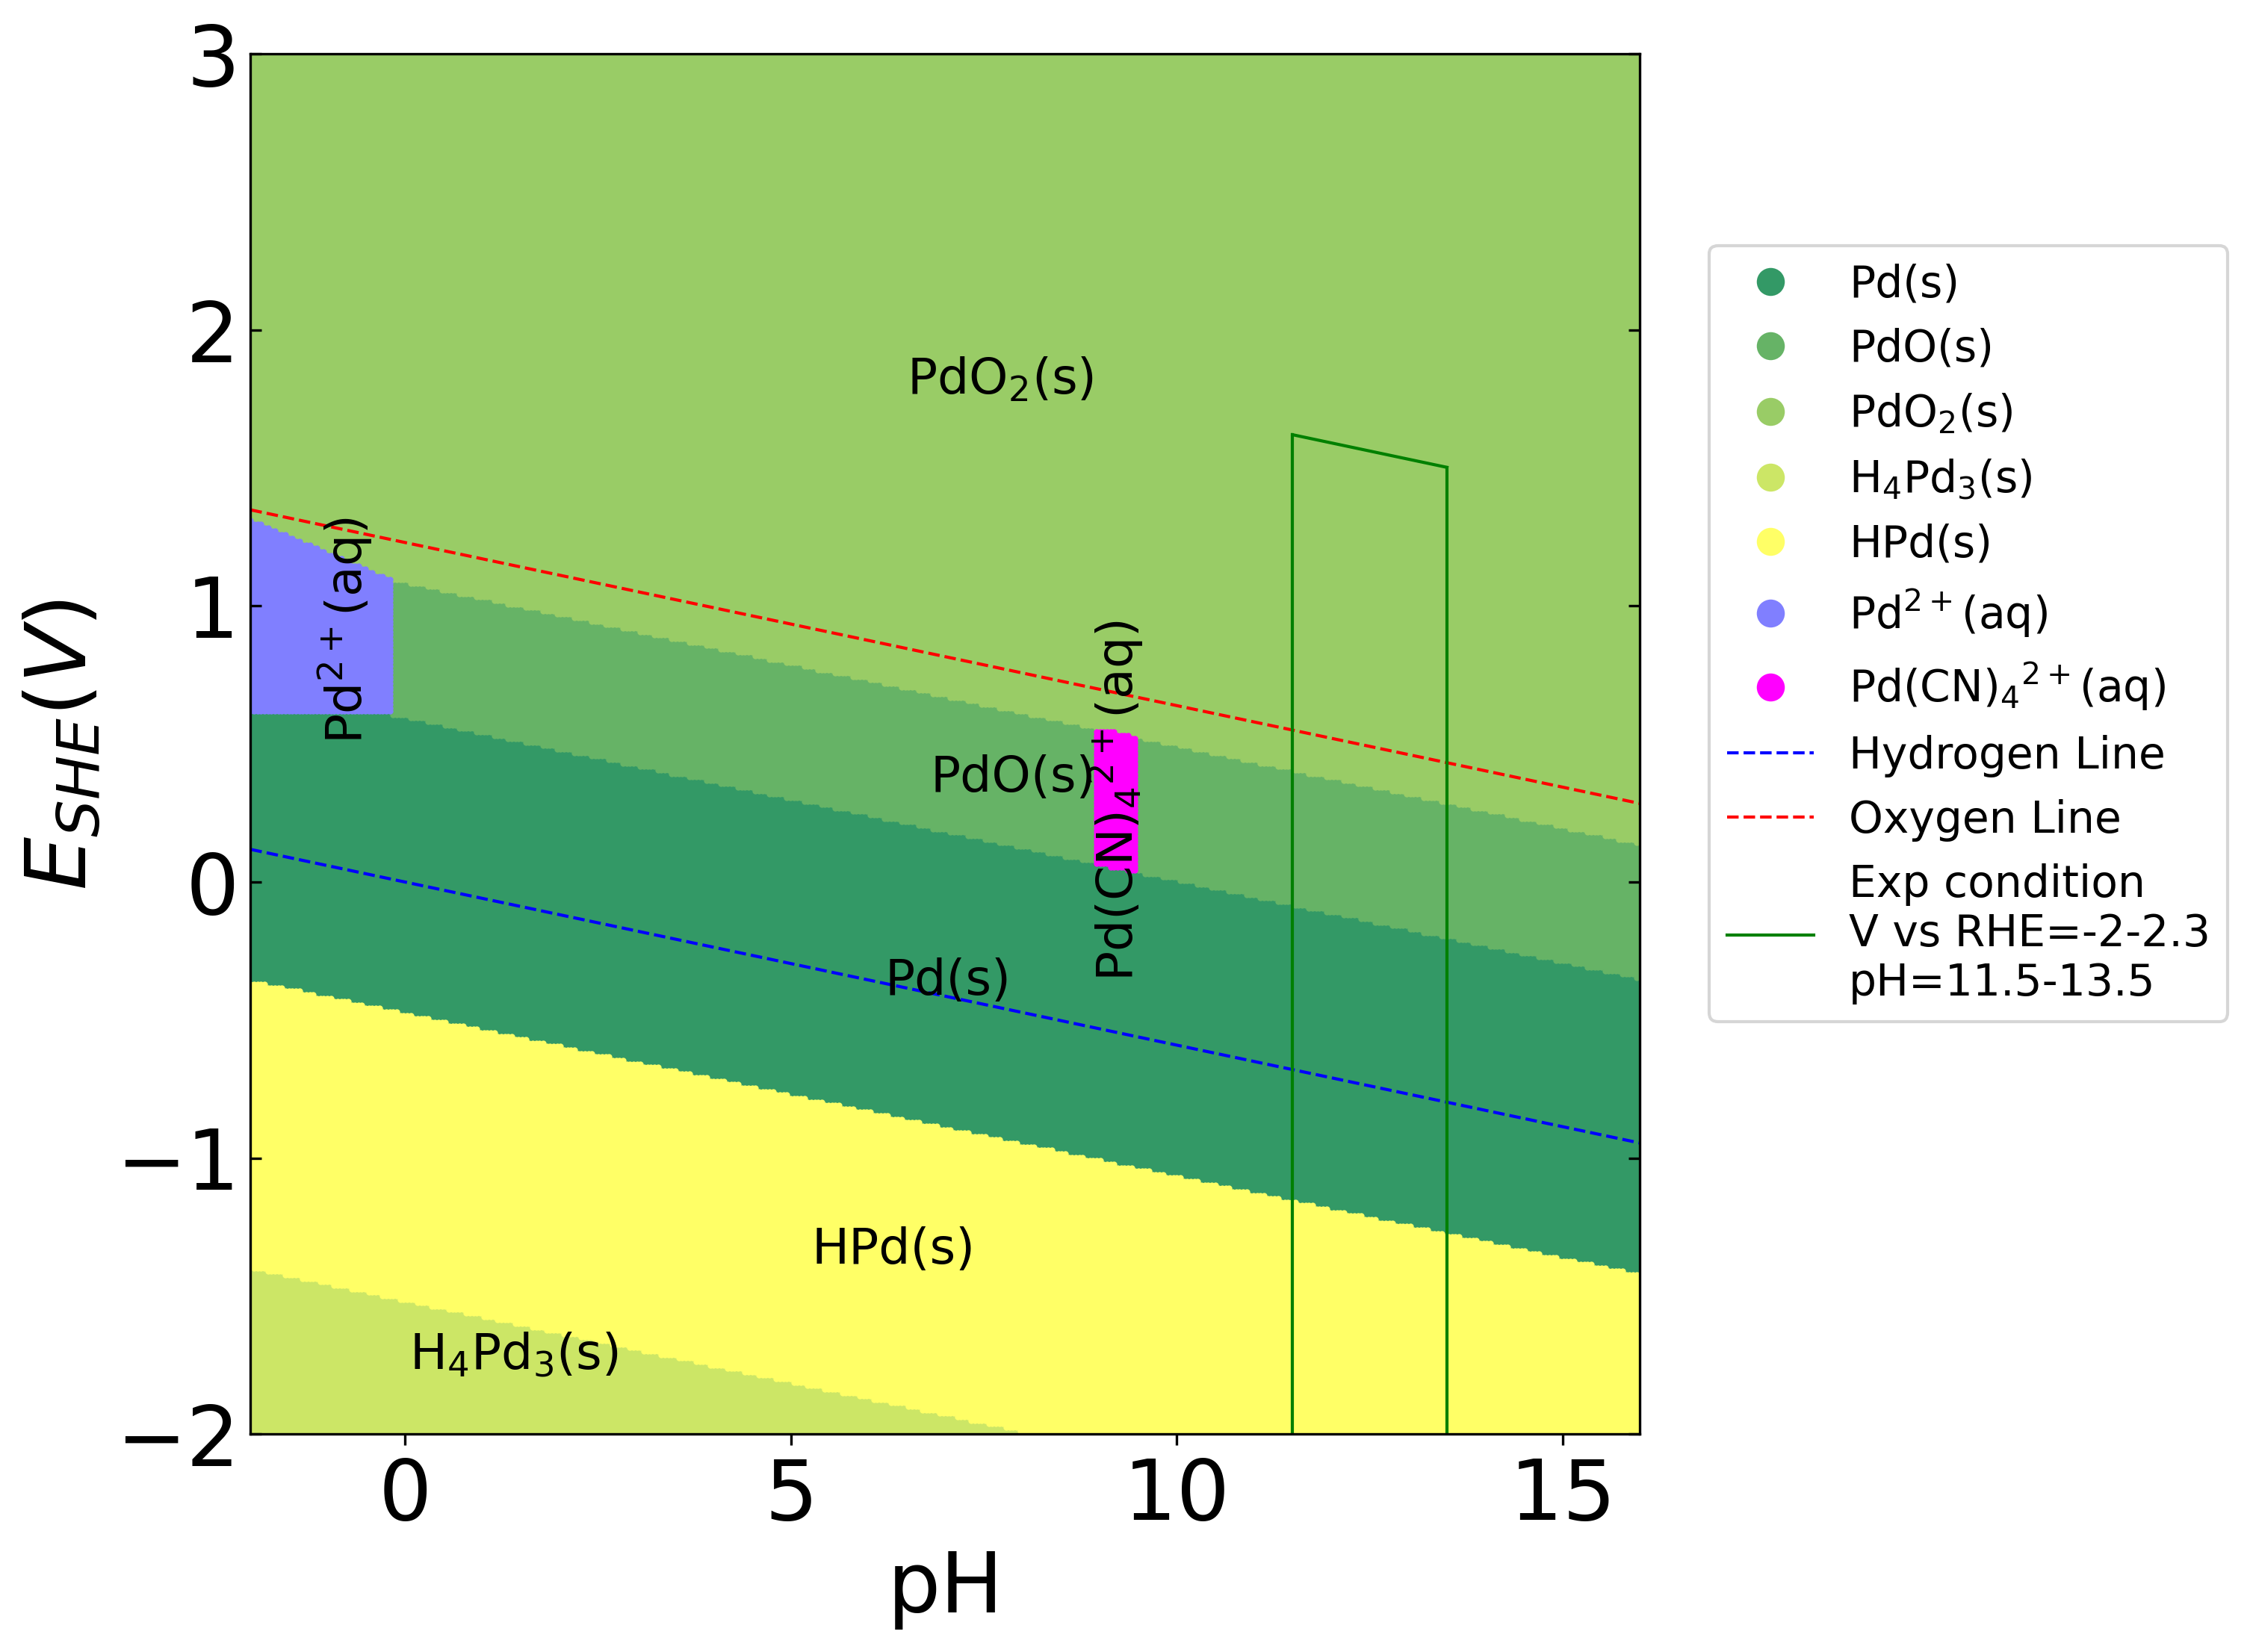
\includegraphics[width=\textwidth]{Figures/pourbaix_diagrams/Pd-NH3-H2O_activity=1e-04_[NH3]=0.02M_[Gly]=0.005M_[CN]=0.0001.png}
%         \subcaption{}\label{fig:Pd_Pourbaix_CN_CH3_Gly}
%     \end{subfigure}
%     % Subfigure (f)
%     \begin{subfigure}[b]{0.3\textwidth}
%         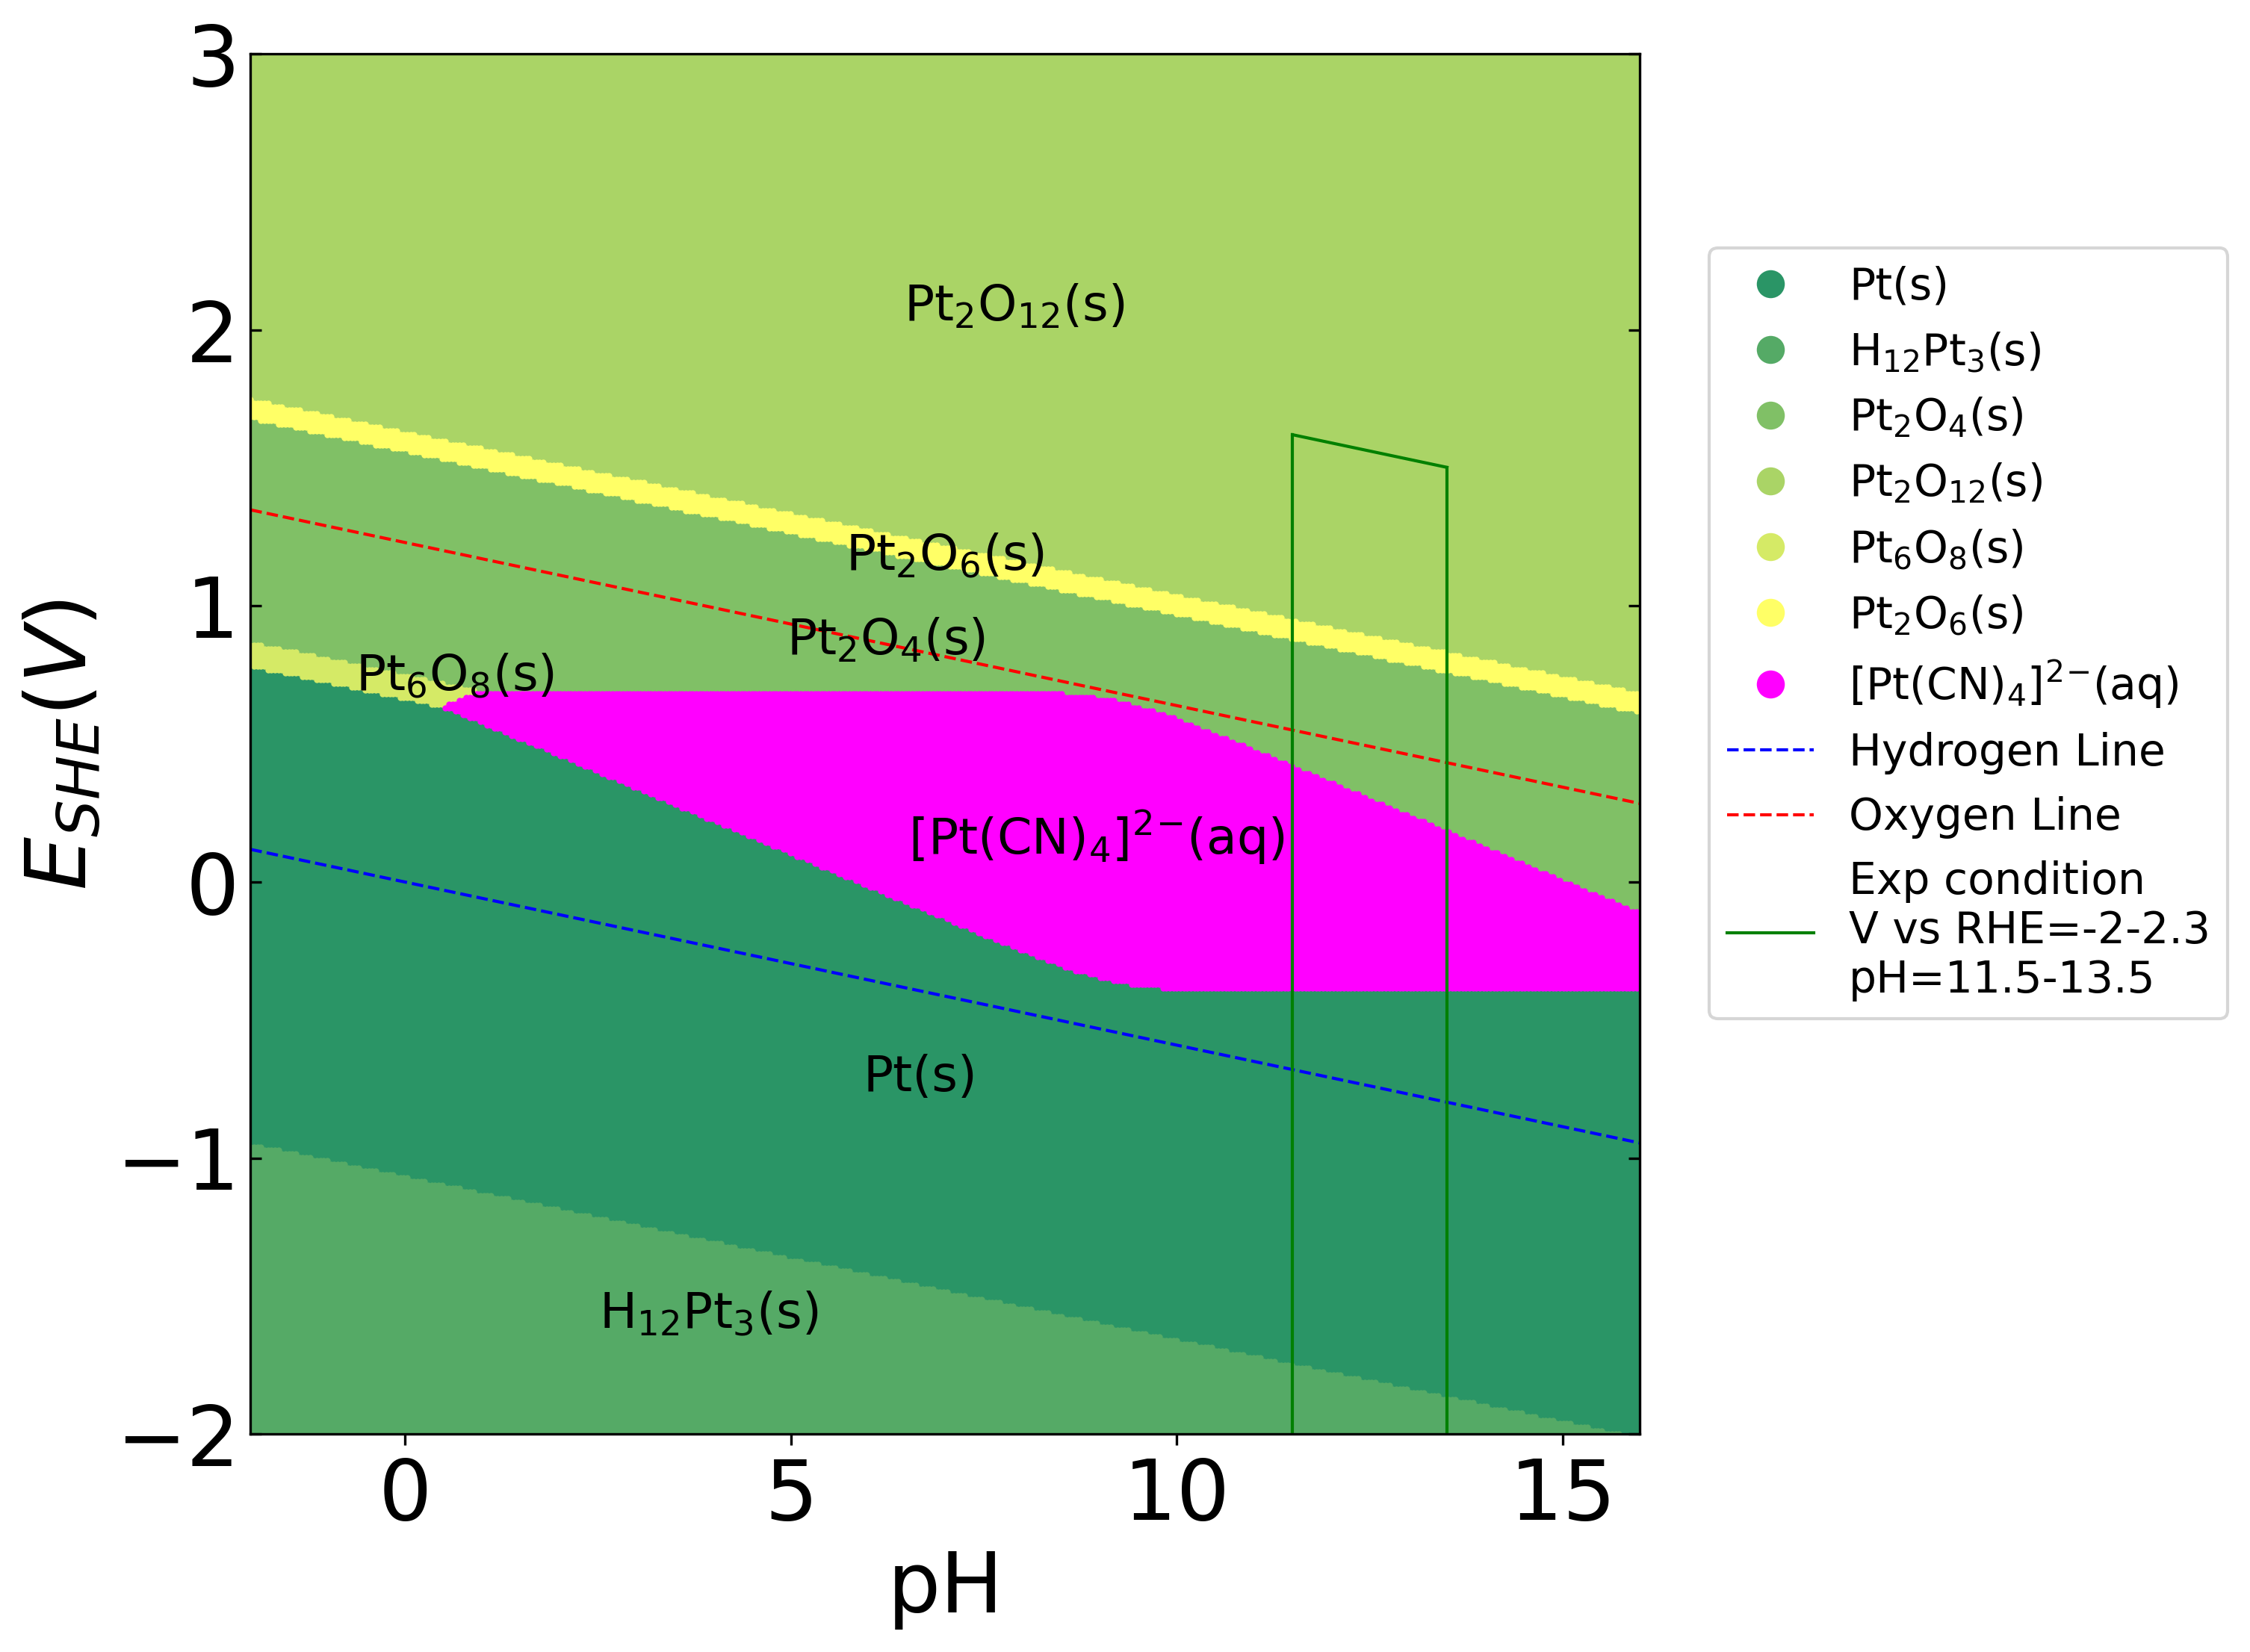
\includegraphics[width=\textwidth]{Figures/pourbaix_diagrams/Pt-NH3-H2O_activity=1e-04_[NH3]=0.02M_[Gly]=0.005M_[CN]=0.0001.png}
%         \subcaption{}\label{fig:Pt_Pourbaix_CN_CH3_Gly}
%     \end{subfigure}

%     \caption{Pourbaix diagrams for metal-\ce{NH3}-\ce{Gly}-\ce{CN-} systems. $[NH_3]_{initial}= \num{2e-2}M$, $[Gly]_{initial}=\num{5e-3}M$, $[\ce{CN-}]_{initial}=\num{1e-4}M$. Green box indicates experimental condition at applied potential vs RHE = -2 to 2 V, pH = 11.5 to 13.5.}
%     \label{fig:Pourbaix_NH3_Gly}
% \end{figure}